\part[Fisica 3]{Fisica 3\\\vspace{1cm}\large{gas, radiazione di corpo nero, calori specifici dei solidi, calori specifici dei gas}}
\begin{savequote}[6cm]
	`Per me si va ne la città dolente,\\ per me si va ne l'etterno dolore,\\ per me si va tra la perduta gente.\\
	\ldots\\
	Dinanzi a me non fuor cose create\\ se non etterne, e io etterno duro.\\ Lasciate ogni speranza, voi ch'intrate'.
	\qauthor{Inferno, canto III}
\end{savequote}
\chapter{Grandezze}
\minitoc
\section{Mole\index{mole}}
\begin{Def}[mole]
	Una mole è definita come la quantità di materia che contiene un numero di elementi uguale al numero di atomi che ci sono in $\SI{12}{\gram}$ di $^{12}\mathrm{C}$. Usando la mole deve essere specificato il tipo di elementi (atomi, molecole, \ldots).
\end{Def}
Segue che una mole di $^{12}\mathrm{C}$ corrisponde a $\SI{12}{\gram}$, ma una mole di $\mathrm{C}$ corrisponde a poco più di $\SI{12}{\gram}$ perché in un campione naturale di $\mathrm{C}$ sono contenuti anche isotopi più pesanti.
\begin{Def}[numero di Avogadro\index{numero!di Avogadro}]
	Il numero di Avogadro è il numero di atomi in $\SI{12}{\gram}$ di $^{12}\mathrm{C}$
\end{Def}
Quindi una mole di una data sostanza corrisponde a un numero di Avogadro di molecole o atomi di quella sostanza.
\section{Unità di massa atomica\index{unità di massa atomica}}
Nel 1815 Proust\index{Proust} propose di introdurre la massa atomica relativa, riferita alla massa dell'idrogeno uguale a $1$. Le masse atomiche degli altri elementi risultano essere molto vicine a numeri interi. Un altro metodo era quello di riferire la massa atomica al sedicesimo delle massa dell'atomo di ossigeno. Oggi ci si riferisce al $^{12}\mathrm{C}$:
\begin{Def}[unità di massa atomica]
	Una massa atomica ($\SI{1}{\atomicmass}$) è pari al dodicesimo della massa del $^{12}\mathrm{C}$.
\end{Def}
Una mole di $^{12}\mathrm{C}$ corrisponde per definizione a $\SI{12}{\gram}$ di carbonio 12 e in essa sono contenuti $N_A$ atomi, quindi la massa di un atomo di $^{12}\mathrm{C}$ è $\SI{12}{\gram}/N_A$, quindi il dodicesimo:
\[
	\SI{1}{\atomicmass} = \frac{\gram\per\mole}{N_A} = \frac{\gram\per\mole}{6.022\ldots\times 10^{23}\;\per\mole}\simeq \SI{1.6605402E-27}{\kilogram}
\]

\chapter{Gas\index{gas}}
\minitoc
\section{Legge dei gas\index{legge!dei gas}}
Utilizzando la teoria del gas perfetto (vedi \ref{gas perfetto} a pag.\@\pageref{gas perfetto}) si dimostra che il prodotto $PV$ è costante:
\begin{equation}
	PV = \frac{2}{3}U
	\label{gas10}
\end{equation}
con $U$ l'energia interna totale di $N$ particelle, legata all'energia cinetica $K$. Essendo il gas perfetto $K=U$. Confrontando la \eqref{gas10} con l'equazione (fenomenologica) dei gas perfetti
\begin{equation}
	PV=nRT
\end{equation}
si scopre che:
\begin{equation}
	U=\frac{3}{2}nRT
\end{equation}
Siamo allora indotti a formulare il principio di equipartizione dell'energia, cioè ad assegnare ad ogni grado di libertà un'energia pari a $\frac{1}{2}NkT$.
\subsection{Gas reali}
Un gas reale è approssimato da un gas ideale tanto più è bassa la sua densità. In questa condizione le ipotesi sul gas ideale sono approssimativamente vere.
\subsubsection{Sviluppo del viriale\index{sviluppo!del viriale}}
\begin{equation}
	pV=nRT\left[1+B_1\frac{n}{V}+B_2\left(\frac{n}{V}\right)^2+\ldots\right]=nRT\sum_{j=0}^\infty B_j\left(\frac{n}{V}\right)^j
\end{equation}
$B_0=1$, $B_1$, $B_2$, \ldots sono detti coefficienti del viriale\index{coefficienti!del viriale}. Essi sono funzione della temperatura e diventano più piccoli al progredire della serie. Se $\frac{n}{V}\to 0$ come per un gas rarefatto si ritrova la legge del gas perfetto.
\subsubsection{Equazione di stato di van der Waals\index{van der Waals}\index{equazione di stato!di van der Waals}}
\begin{equation}
	\left(p+\frac{an^2}{V^2}\right)(V-nb)=nRT
\end{equation}
è uguale all'equazione di stato considerando un volume ridotto e una pressione aumentata. Nel gas perfetto si assume che il volume occupato dalle molecole sia trascurabile, questo non è del tutto vero e quindi il volume che consideriamo nell'equazione dei gas perfetti è sovrastimato, va quindi diminuito. In altre parole il volume libero per il movimento delle molecole è più piccolo. Consideriamo due molecole di diametro $d$. Possiamo schematizzarle come una molecola puntiforme e una di diametro $2d$ o raggio $d$. Quindi il volume a disposizione della molecola puntiforme è ridotto di $\frac{4}{3}\pi d^3$. Essendo le molecole due per ogni molecola è sottratto un volume pari a:
\begin{equation}
	\frac{4}{3}\pi\frac{d^3}{2}=4\left[\frac{4}{3}\pi\left(\frac{d}{2}\right)^3\right]
\end{equation}
cioè 4 volte il volume della molecola. Per una mole, cioè un numero di Avogadro di molecole, il volume sottratto al movimento, cioè il covolume $b$, è:
\begin{equation}
	b=4N_A\left[\frac{4}{3}\pi\left(\frac{d}{2}\right)^3\right]
	\label{covolume02}
\end{equation}
In realtà per alte pressioni le molecole sono molto più vicine e il $4$ che compare nell'espressione \eqref{covolume02} può ridursi notevolmente. Per $n$ moli il volume in meno è $nb$.

Per quanto riguarda la pressione per il gas perfetto si assume che non ci siano forze intermolecolari. Su una molecola mediamente il contributo di queste forze sarà nullo, tranne per quelle che si trovano sul bordo, su di queste agirà una forza netta verso l'interno, quindi la pressione (sulle pareti) va diminuita rispetto a quella del gas ideale. La forza è proporzionale al numero di molecole presenti nell'emisfero di raggio $R$ in cui ha efficacia la forza attrattiva, a sua volta proporzionale alla densità molecolare e quindi alla densità molare $\frac{n}{V}$ L'effetto sommato per tutte le molecole è anch'esso proporzionale alla densità molecolare e quindi a $\frac{n}{V}$. La riduzione di pressione complessiva è quindi proporzionale a $\left(\frac{n}{V}\right)^2$.
\section{Distribuzione delle velocità\index{distribuzione!delle velocità}}
\subsection{Distribuzioni delle componenti}
Consideriamo un gas ideale chiuso in un recipiente, mantenuto ad una temperatura $T$.
Vogliamo sapere quante molecole hanno una certa velocità compresa tra $v_x$ e $v_x+\ud v_x$ lungo un asse, per esempio l'asse $x$. Indichiamo con $f_x$ la funzione densità di probabilità della variabile casuale $v_x$ che ha dominio $\field{R}$. Ipotesi iniziali:
\begin{enumerate}
	\item lo spazio è isotropo;\label{ipotesi_max_uno}
	\item la distribuzione delle velocità lungo un asse non è influenzata dalle componenti sugli altri assi;\label{ipotesi_max_due}
	\item la velocità quadratica media è $v_{qm}=\sqrt{\media{v^2}}=\sqrt{\frac{3kT}{m}}$;\label{ipotesi_max_tre}
\end{enumerate}
L'ipotesi \ref{ipotesi_max_uno} deriva dal fatto che il moto delle molecole è casuale, la \ref{ipotesi_max_tre} deriva dall'energia di un gas ideale $U=\frac{3}{2}kT=\media{\frac{1}{2}mv^2}=\frac{1}{2}m\media{v^2}$. La prima ipotesi significa che:
\begin{equation}
	f_x(v_x,v_y,v_z)=f_y(v_x,v_y,v_z)=f_z(v_x,v_y,v_z)
\end{equation}
ma anche che:
\begin{equation}
	f_x(-v_x,v_y,v_z)=f_x(v_x,v_y,v_z)
\end{equation}
o più in generale che ogni distribuzione è una funzione pari per ogni argomento.
La seconda ipotesi si traduce in:
\begin{equation}
	f_x=f_x(v_x)
\end{equation}
e analogamente per le altre.

Essendo le tre distribuzioni delle componenti uguali:
\begin{equation}
	\media{v_x^2}=\media{v_y^2}=\media{v_z^2}
\end{equation}
quindi:
\begin{equation}
	\media{v^2}=\media{v_x^2+v_y^2+v_z^2}=\media{v_x^2}+\media{v_y^2}+\media{v_z^2}=3\media{v_x^2}
\end{equation}
e allora:
\begin{equation}
	\media{v_x^2}=\frac{kT}{m}
\end{equation}


Se $f_x$ è la densità di probabilità allora è normalizzata a $1$. $Nf_x$ è normalizzata ad $N$ numero di molecole. Possiamo scrivere:
\[\ud P(v_x) = f(v_x)\,\ud v_x\]
oppure
\[\ud N(v_x) = Nf(v_x)\,\ud v_x\]
Allora:
\begin{equation}
	N\int_{v_{x_1}}^{v_{x_2}} f(v_x)\,\ud v_x
\end{equation}
sarà il numero di molecole con velocità lungo l'asse $x$ compresa tra $v_{x_1}$ e $v_{x_2}$.

La funzione distribuzione di probabilità di $\ve v$ utilizzando la probabilità composta di eventi indipendenti (ipotesi \ref{ipotesi_max_due}) sarà:
\begin{equation}
	F(\ve v)=F(v_x,v_y,v_z)=f_x(v_x)f_y(v_y)f_z(v_z)
	\label{distr_F01}
\end{equation}
Quello che vogliamo fare ora trovare la distribuzione più probabile, quindi dovremo massimizzare $F$. Poiché il logaritmo è una funzione crescente possiamo massimizzare il logaritmo di $F$. Il differenziale del logaritmo della \eqref{distr_F01}:
\begin{equation}
	\begin{split}
		\ud \log F=&\ud\left(\log f_x(v_x)+\log f_y(v_y)+\log f_z(v_z)\right)\\
		=&\frac{f'_x(v_x)}{f_x(v_x)}\ud v_x+\frac{f'_y(v_y)}{f_y(v_y)}\ud v_y+\frac{f'_z(v_z)}{f_z(v_z)}\ud v_z
	\end{split}
\end{equation}
usando i moltiplicatori di Lagrange con il vincolo su $v^2$ e quindi\footnote{più precisamente il vincolo è la funzione:
	\begin{equation}
		G(v_x,v_y,v_z)=v_x^2+v_y^2+v_z^2-\frac{3kT}{m}=0
	\end{equation}
}:
\begin{equation}
	\left\{
	\begin{array}{l}
		\frac{\partial\log F}{\partial v_x}=\frac{f'_x(v_x)}{f_x(v_x)}=\lambda\frac{\partial(v^2)}{\partial v_x}=2\lambda v_x \\
		\frac{\partial\log F}{\partial v_y}=\frac{f'_y(v_y)}{f_y(v_y)}=\lambda\frac{\partial(v^2)}{\partial v_y}=2\lambda v_y \\
		\frac{\partial\log F}{\partial v_z}=\frac{f'_z(v_z)}{f_z(v_z)}=\lambda\frac{\partial(v^2)}{\partial v_z}=2\lambda v_z \\
	\end{array}
	\right.
\end{equation}
preoccupiamoci solo della prima, abbiamo già dimostrato che $f_x=f_y=f_z$:
\begin{equation}
	\frac{f'_x(v_x)}{f_x(v_x)}=-2\lambda v_x
\end{equation}
risolvendo l'equazione differenziale e scrivendo $\lambda$ al posto di $2\lambda$:
\begin{equation}
	\log f_x=-\lambda v_x^2+c
\end{equation}
ovvero:
\begin{equation}
	f_x(v_x)=f_{0x}e^{-\lambda v_x^2}
\end{equation}
con $f_{0x}$ e $\lambda$ costanti da determinare dal vincolo.
\subsection{Determinazione costanti}
\subsubsection{Integrali di Gauss\index{Gauss}\index{integrali!di Gauss}}
Calcoliamo:
\begin{equation}
	\int_{-\infty}^{+\infty}e^{-A^2x^2}\,\ud x
\end{equation}
di questo integrale non esiste primitiva analitica, definiamo $I_0$ l'integrale, calcoliamo:
\begin{equation}
	\begin{split}
		I_0^2=&\int_\field{R}e^{-A^2x^2}\,\ud x\int_\field{R}e^{-A^2y^2}\,\ud y=\iint_{\field{R}^2}e^{-A^2(x^2+y^2)}\,\ud x\ud y\\
		=&\int_0^\infty\int_0^{2\pi} e^{-A^2\rho^2}\rho\ud\rho\ud\theta=2\pi\int_0^\infty e^{-A^2\rho^2}\rho\ud \rho=\frac{\pi}{A^2}
	\end{split}
\end{equation}
quindi:
\begin{equation}
	\int_{-\infty}^{+\infty}e^{-A^2x^2}\,\ud x=\frac{\sqrt{\pi}}{A}
\end{equation}
Definiamo:
\begin{equation}
	I_2=\int_{-\infty}^{+\infty}x^2e^{-A^2x^2}\,\ud x
\end{equation}
e in modo analogo $I_4$, $I_6$, \ldots Notiamo che $I_2=-\frac{\partial I_0}{\partial A^2}$, infatti:
\begin{equation}
	-\frac{\partial}{\partial A^2}\int_\field{R}e^{-A^2x^2}\,\ud x=-\int_\field{R}\frac{\partial}{\partial A^2}e^{-A^2x^2}\,\ud x=\int_\field{R}x^2e^{-A^2x^2}\ud x=I_2
\end{equation}
Allora:
\begin{equation}
	I_2=-\frac{\partial}{\partial A^2}I_0=\frac{\partial}{\partial A^2}\frac{\sqrt{\pi}}{A}=\frac{\sqrt{\pi}}{2A^3}
\end{equation}
si può dimostrare che:
\begin{equation}
	I_n=-\frac{\partial I_{n-2}}{\partial A^2}
\end{equation}
con $n$ pari. Per quelli dispari\footnote{vengono definiti su $\field{R}^+$, perché essendo funzioni dispari l'integrale su $\field{R}$ è nullo} banalmente:
\begin{equation}
	I_1=\int_0^{\infty}xe^{-A^2x^2}\,\ud x=\frac{1}{2A^2}
\end{equation}
si nota che:
\begin{equation}
	\begin{split}
		I_3=&-\frac{\partial I_1}{\partial A^2}=-\frac{\partial}{\partial A^2}\int_0^\infty xe^{-A^2x^2}\,\ud x=\int_0^{\infty}-\frac{\partial}{\partial A^2}\left(xe^{-A^2x^2}\right)\,\ud x\\
		=&\int_0^\infty x^3e^{-A^2 x^2}\ud x
	\end{split}
\end{equation}
quindi:
\begin{equation}
	I_3=-\frac{\partial I_1}{\partial A^2}=\frac{1}{2A^4}
	\label{Itre}
\end{equation}
\subsubsection{Determinazione costanti}
Imponiamo la normalizzazione e la velocità quadrata media:
\begin{equation}
	\int_{-\infty}^{+\infty}f(v_x)\,\ud v_x=1\qquad\media{v_x^2}=\frac{kT}{m}
\end{equation}
\begin{equation}
	\int_{-\infty}^{+\infty}f_0e^{-A^2v_x^2}\,\ud v_x=f_0\int_{-\infty}^{+\infty}e^{-A^2v_x^2}\,\ud v_x=f_0 \frac{\sqrt{\pi}}{A}=1
\end{equation}
si ricava:
\begin{equation}
	f_0=\frac{A}{\sqrt{\pi}}
\end{equation}
siamo arrivati a:
\begin{equation}
	f(v_x)=\frac{A}{\sqrt{\pi}}e^{-A^2v_x^2}
\end{equation}
Imponiamo la velocità quadrata media:
\begin{equation}
	\int_\field{R}v_x^2 f(v_x)\,\ud v_x=\int_\field{R}v_x^2\frac{A}{\sqrt{\pi}}e^{-A^2v_x^2}\,\ud v_x=\frac{A}{\sqrt{\pi}}\frac{\sqrt{\pi}}{2A^3}=\frac{1}{2A^2}=\frac{kT}{m}
\end{equation}
si ricava:
\begin{equation}
	A=\sqrt{\frac{m}{2kT}}
\end{equation}
La distribuzione delle componenti risulta allora:
\begin{equation}
	f(v_x)=\sqrt{\frac{m}{2\pi kT}}\,e^{-\dfrac{mv_x^2}{2kT}}
\end{equation}
e analogamente per le altre componenti. Si noti come argomento dell'esponenziale decrescente sia il rapporto tra l'energia cinetica ($\frac{1}{2}mv_x^2$) e $kT$.
\subsection{Distribuzione dei moduli}
Dati $v_x$, $v_y$, $v_z$ siamo in grado di dare la distribuzione di probabilità:
\begin{equation}
	f(v_x)f(v_y)f(v_z)=\left(\frac{m}{2\pi kT}\right)^{\frac{3}{2}}e^{-\frac{mv_x^2}{2kT}}e^{-\frac{mv_y^2}{2kT}}e^{-\frac{mv_z^2}{2kT}}=\left(\frac{m}{2\pi kT}\right)^{\frac{3}{2}}e^{-\frac{mv^2}{2kT}}
	\label{distr_moduli13}
\end{equation}
questa non è la distribuzione che stiamo cercando, infatti fissato $v$ ci sono infiniti vettori $\ve v$ tali che $\norm{\ve v}=v$. Questi vettori stanno su una superficie sferica. Dobbiamo integrare sulla superficie sferica, ma siamo fortunati perché la \eqref{distr_moduli13} ha simmetria sferica:
\begin{equation}
	f(v)=\left(\frac{m}{2\pi kT}\right)^{\frac{3}{2}}e^{-\frac{mv^2}{2kT}}4\pi v^2
\end{equation}
\subsubsection{velocità più probabile\index{velocità!più probabile}}
\begin{equation}
	\frac{\ud f}{\ud v}
	=\Bigl(\ldots\Bigr)^{\frac{3}{2}}4\pi\left[2v_p\left(e^{-\frac{m v_p^2}{2kT}}\right)+v_p^2e^{-\frac{mv_p^2}{2kT}}\left(-\frac{2v_p m}{2kT}\right)\right]=0
\end{equation}
\begin{equation}
	v_p=\sqrt{\frac{2kT}{m}}
\end{equation}
che è effettivamente un massimo.
\subsubsection{velocità media\index{velocità!media}}
\begin{equation}
	\begin{split}
		\overline{v}=&\int_{\field{R}^+}vf(v)\,\ud v=\int_{\field{R}^+}4\pi v^3\left(\frac{m}{2\pi kT}\right)^{\frac{3}{2}}e^{-\frac{mv^2}{2kT}}\,\ud v\\
		=&{4\pi}\left(\frac{m}{2\pi kT}\right)^{\frac{3}{2}}\int_0^{+\infty}v^3e^{-\frac{mv^2}{2kT}}\,\ud v=4\pi\left(\frac{m}{2\pi kT}\right)^{\frac{3}{2}}\left(\frac{4k^2T^2}{2m^2}\right)\\
		=&\sqrt{\frac{8kT}{\pi m}}
	\end{split}
\end{equation}
avendo usato la \eqref{Itre}.
\subsubsection{velocità quadratica media\index{velocità!quadratica media}}
sappiamo già che la velocità quadrata media è $\frac{3kT}{m}$, ma calcoliamolo:
\begin{equation}
	\begin{split}
		\media{v^2}&=\int_{\field{R}^+} v^2f(v)\,\ud v=\int_{\field{R}^+}4\pi v^4\left(\frac{m}{2\pi kT}\right)^{\frac{3}{2}}e^{-\frac{mv^2}{2kT}}\,\ud v\\
		&=\frac{1}{2}\int_{\field{R}}4\pi v^4\left(\frac{m}{2\pi kT}\right)^{\frac{3}{2}}e^{-\frac{mv^2}{2kT}}\,\ud v=
		2\pi\left(\frac{m}{2\pi kT}\right)^{\frac{3}{2}}\int_{\field{R}}v^4e^{-\frac{mv^2}{2kT}}\,\ud v\\
		&=\frac{2}{\sqrt{\pi}}\left(\frac{m}{2 kT}\right)^{\frac{3}{2}}\frac{3}{4}\left(\frac{2kT}{m}\right)^{\frac{5}{2}}=\frac{3kT}{m}
	\end{split}
\end{equation}
in quanto $I_4=\frac{3\sqrt{\pi}}4{A^5}$, la velocità quadratica media:
\begin{equation}
	v_{qm}=\sqrt{\frac{3kT}{m}}
\end{equation}
esaminando i coefficienti ($\frac{8}{\pi}\simeq 2.5$) risulta:
\begin{equation}
	v_p<\overline{v}<v_{qm}
\end{equation}
\subsection{Distribuzione dell'energia\index{distribuzione delle energie}}
Avendo fissato la massa di una particella la relazione che lega il modulo della velocità all'energia della particella è biunivoca\footnote{non farsi ingannare dal quadrato: la velocità può essere solo positiva $E:\field{R}^+\to\field{R}^+$}:
\begin{equation}
	E=\frac{1}{2}mv^2
	\label{cinetica_Edistr}
\end{equation}
possiamo passare dalla distribuzione dei moduli delle velocità alla distribuzione dell'energia. Partendo dalla distribuzione dei moduli:
\begin{equation}
	f(v)=\frac{\ud P}{\ud v}=4\pi v^2\left(\frac{m}{2\pi kT}\right)^{\frac{3}{2}}e^{-\frac{mv^2}{2kT}}
\end{equation}
\begin{equation}
	{\ud P}=4\pi v^2\left(\frac{m}{2\pi kT}\right)^{\frac{3}{2}}e^{-\frac{mv^2}{2kT}}{\ud v}
	\label{moduli_Edistr}
\end{equation}
dalla \eqref{cinetica_Edistr} possiamo ricavare $v(E)$ e $\ud v(\ud E)$:
\begin{equation}
	v=\sqrt{\frac{2E}{m}}\qquad \ud v=\frac{\ud E}{mv}=\sqrt{\frac{1}{2Em}}\ud E
\end{equation}
sostituendo nella \eqref{moduli_Edistr} e semplificando:
\begin{equation}
	g(E)=\frac{\ud P}{\ud E}=2\sqrt{E}\sqrt{\frac{1}{\pi k^3T^3}}e^{-\dfrac{E}{kT}}
\end{equation}
\subsubsection{Energia più probabile}
\begin{equation}
	\frac{\ud}{\ud E}g(E_p)=0\qquad
	E_p=\frac{3}{2}kT
\end{equation}
\subsubsection{Energia media}
\begin{equation}
	\media{E}=\int_{\field{R}^+} Eg(E)\,\ud E=\frac{3}{2}kT
\end{equation}
\subsubsection{Energia quadratica media}
\begin{equation}
	E_{qm}=\sqrt{\int_{\field{R}^+} E^2 g(E)\,\ud E}=\sqrt{\frac{15}{4}}kT
\end{equation}
\section{Effetto Doppler termico}
L'effetto Doppler non trasversale di una sorgente in movimento con velocità $v$ verso l'osservatore fermo è:
\begin{equation}
	\nu=\nu_0\frac{(1+\beta)}{\sqrt{1-\beta^2}}
\end{equation}
con $\nu$ la frequenza apparente e $\nu_0$ la frequenza propria della sorgente, $\beta=\frac{v}{c}$. Se consideriamo $v\ll c$ allora:
\begin{equation}
	\nu\sim \nu_0(1+\beta)\left(1+\frac{1}{2}\beta^2\right)=\nu_0\left(1+\frac{1}{2}\beta^2+\beta+\frac{1}{2}\beta^3\right)
\end{equation}
trascurando gli infinitesimi di ordine superiore:
\begin{equation}
	\nu=\nu_0\left(1+\frac{v}{c}\right)
	\label{doppler_termico01}
\end{equation}
Consideriamo ora un forno con una finestra di quarzo molto piccola dal quale esca della radiazione emessa dalle molecole all'interno con distribuzione delle velocità:
\begin{equation}
	\ud N=N\left(\frac{m}{2\pi kT}\right)^{\frac{1}{2}}e^{-\frac{mv_x^2}{2kT}}\,\ud v_x
	\label{doppler_termico02}
\end{equation}
ipotizzando che noi possiamo vedere solo la radiazione emessa da molecole con velocità nella direzione $x$. Passiamo dalla distribuzione delle velocità alla distribuzione in frequenza usando la relazione \eqref{doppler_termico01} con $v=v_x$:
\begin{equation}
	v_x=\left(\frac{\nu}{\nu_0}-1\right)c\qquad \ud v_x=c\frac{\ud \nu}{\nu_0}
\end{equation}
sostituendo nella \eqref{doppler_termico02}:
\begin{equation}
	\ud N=N\left(\frac{m}{2\pi kT}\right)^{\frac{1}{2}}e^{-\frac{m\left(\frac{\nu}{\nu_0}-1\right)^2 c^2}{2kT}}c\frac{\ud \nu}{\nu_0}=N\left(\frac{m}{2\pi kT}\right)^{\frac{1}{2}}e^{\frac{-mc^2\left(\nu-\nu_0\right)^2}{2kT\nu_0^2}}\frac{c}{\nu_0}\,\ud\nu
\end{equation}
essendo l'intensità proporzionale a $n$ analizzando lo spettro di emissione di un gas non si ottengono delle righe infinitamente sottili, ma delle gaussiane:
\begin{equation}
	I(\nu)\propto \frac{\ud N}{\ud \nu}=N\left(\frac{m}{2\pi kT}\right)^{\frac{1}{2}}e^{\frac{-mc^2\left(\nu-\nu_0\right)^2}{2kT\nu_0^2}}\frac{c}{\nu_0}
\end{equation}
\subsection{Risoluzione}
Calcoliamo il massimo della gaussiana (l'altezza):
\begin{equation}
	I_{\max}(\nu)\propto N\left(\frac{m}{2\pi kT}\right)^{\frac{1}{2}}\frac{c}{\nu_0}
\end{equation}
La larghezza a metà altezza:
\[
	I=\frac{I_{\max}}{2}\qquad N\left(\frac{m}{2\pi kT}\right)^{\frac{1}{2}}e^{\frac{-mc^2\left(\nu-\nu_0\right)^2}{2kT\nu_0^2}}\frac{c}{\nu_0}=\frac{1}{2}N\left(\frac{m}{2\pi kT}\right)^{\frac{1}{2}}\frac{c}{\nu_0}
\]
\[
	e^{\frac{-mc^2\left(\nu-\nu_0\right)^2}{2kT\nu_0^2}}=\frac{1}{2}\qquad \frac{mc^2\left(\nu-\nu_0\right)^2}{2kT\nu_0^2}=\log 2
\]
quindi:
\begin{equation}
	\nu_{1/2}=\nu_0\pm\sqrt{\frac{2kT\nu_0^2\log 2}{mc^2}}=\nu_0\pm\frac{\nu_0}{c}\sqrt{\frac{2kT\log 2}{m}}
\end{equation}
quindi l'ampiezza della campana a metà altezza è:
\begin{equation}
	\Delta \nu_{1/2}=2\frac{\nu_0}{c}\sqrt{\frac{2kT\log 2}{m}}
\end{equation}
la risoluzione:
\begin{equation}
	\frac{\Delta \nu_{1/2}}{\nu_0}=\frac{2}{c}\sqrt{\frac{2kT\log 2}{m}}
\end{equation}
che va come $\sqrt{\frac{T}{m}}$.
\section{Libero cammino medio}
Sappiamo\footnote{vedi \ref{libero cammino medio fisica1} a pag.\@\pageref{libero cammino medio fisica1}} che se consideriamo tutte le molecole ferme e solo una in moto, il libero cammino di questa è:
\begin{equation}
	L=\frac{1}{n\pi d^2}=\frac{1}{n\sigma}
\end{equation}
con $n$ il numero di molecole per volume, $d$ il diametro molecolare, $\sigma=\pi d^2$ la sezione d'urto. Se le altre molecole si muovono dobbiamo considerare la velocità relativa. Rifacendo tutto il ragionamento: la molecola spazza in un tempo infinitesimo $\ud t$ un cilindro di lunghezza $v\ud t$ e quindi volume $\pi d^2 v\ud t$. Il numero di urti sarà uguale al numero di particelle all'interno del cilindro. Se consideriamo la velocità relativa è più corretto:
\begin{equation}
	\label{eq:libero_cammino_medio_rif}
	L=\frac{1}{\sqrt{2}n\sigma}
\end{equation}
\subsection{Calcolo della velocità relativa media}
\label{calcolo_vel_rel_med}
Per calcolare la velocità relativa media bisogna mediare sia sull'angolo tra le direzioni di due molecole che sulla velocità delle due. Siano $\ve u$, $\ve v$ le velocità di due molecole rispetto ad un'osservatore inerziale con il contenitore del gas. La velocità della seconda molecola rispetto alla prima, è:
\[
	\ve r = \ve v - \ve u \qquad \norm{r} = \sqrt{(\ve v-\ve u)^2} = \sqrt{v^2+u^2-2vu\cos(\theta)}
\]
dove $\theta$ è l'angolo tra le due velocità misurato nel sistema dell'osservatore. Se supponessimo che le velocità siano uguali e ad un valore fisso ($v=u$) allora:
\[
	r = \sqrt{2}v\sqrt{1-\cos(\theta)}
\]
Mediando sull'angolo\footnote{si ricorda che l'angolo solido infinitesimo è $\ud\Omega=\sin\theta\,\ud\theta\,\ud\varphi$}:
\begin{align*}
	\left.\media{r}_{\theta}\right|_{u=v} = & \frac{1}{4\pi}\int r\,\ud\Omega                                                                   \\
	=                                       & \frac{1}{4\pi}\sqrt{2}v\int_0^{2\pi}\ud\varphi\int_0^\pi \ud\theta\sin\theta\sqrt{1-\cos(\theta)} \\
	=                                       & -\frac{1}{2}\sqrt{2}v\int_{1}^{-1} \sqrt{1-y}\,\ud y                                              \\
	=                                       & \frac{1}{2}\sqrt{2}v\int_0^{\sqrt{2}} 2z^2\,\ud z                                                 \\
	=                                       & \sqrt{2}v\left.\frac{z^3}{3}\right|_0^{\sqrt{2}}=\frac{4}{3}v
\end{align*}
Questo non è il risultato corretto, ma numericamente ci assomiglia. Considerando invece velocità diverse:
\begin{align*}
	\media{r}_\theta = & \frac{1}{4\pi}\int r\,\ud\Omega                                                     \\
	=                  & \frac{2\pi}{4\pi}\int_0^\pi \sqrt{v^2+u^2-2vu\cos(\theta)}\sin\theta\,\ud\theta     \\
	=                  & -\frac{1}{2}\sqrt{v^2+u^2-2uvy}\,\ud y                                              \\
	=                  & -\frac{1}{2}\int_{\sqrt{v^2+u^2-2uv}}^{\sqrt{v^2+u^2+2uv}} z (-\frac{z}{uv})\,\ud z \\
	=                  & \frac{1}{2uv}\int_{|v+u|}^{v+u} z^2\,\ud z                                          \\
	=                  & \frac{(v+u)^3-|v-u|^3}{6uv}=\begin{cases}
		\frac{1}{3u}(3u^2+v^2) & v \leq u \\
		\frac{1}{3v}(u^2+3v^2) & v \geq u
	\end{cases}
\end{align*}
questa è la media nell'angolo, ora bisogna mediare sulle velocità usando la distribuzione delle velocità di Maxwell. Mediamo su $u$ usando la distribuzione delle velocità:
\[
	f(v)=\frac{4v^2}{\sqrt{\pi}v_p^3} e^{-v^2/v_p^2}
\]
dove è stata introdotta per comodità la velocità più probabile: $v_p=\sqrt{\frac{2kT}{m}}$. Mediando su $v$:
\begin{equation}
	\label{eq:libero_difficile}
	\begin{aligned}
		\media{r}_{\theta,\norm{v}} & = \int_0^\infty f(v) \media{r}_\theta\,\ud v                                                                                                               \\
		                            & = \frac{4}{\sqrt{\pi}v_p^3} \left[\int_0^u v^2 e^{-v^2/v_p^2}\frac{3u^2+v^2}{3u}\,\ud v+ \int_u^\infty v^2 e^{-v^2/v_p^2}\frac{u^2+3v^2}{3v}\,\ud v\right]
	\end{aligned}
\end{equation}
Questo integrale è abbastanza complicato. Iniziamo con una definizione:
\begin{equation}
	\erf(x) = \frac{2}{\pi}\int_0^x e^{-t^2}\,\ud t\qquad \int e^{-x^2}\,\ud x = \frac{\pi}{2}\erf(x)
\end{equation}
dove $\erf(x)$ è la funzione dell'errore. Calcoliamo questa primitiva:
\begin{equation}
	\begin{aligned}
		\int x^2 e^{-x^2}\,\ud x & = \int x (x e^{-x^2})\,\ud x = \frac{1}{2}\left[-e^{-x^2} x + \int e^{-x^2}\,\ud x\right] \\
		                         & = -\frac{1}{2}e^{-x^2}x+\frac{\sqrt{\pi}}{4}\erf(x)
	\end{aligned}
\end{equation}
che serve per calcolare la prima parte del primo integrale nell'equazione \ref{eq:libero_difficile}:
\begin{equation}
	\int_0^u v^2 e^{-v^2/v_p^2}\,\ud v =
	v_p^3\int_0^{u/v_p} y^2 e^{-y^2}\,\ud y =
	\frac{v_p^2}{4}\left[-2 e^{-u^2/v_p^2} u+\sqrt{\pi}v_p\erf\left(\frac{u}{v_p}\right)\right]
\end{equation}
Per il secondo pezzo serve questa primitiva:
\begin{equation}
	\begin{aligned}
		\int x^4 e^{-x^2}\,\ud x & = \int x^3 (x e^{-x^2})\,\ud x = -\frac{1}{2}e^{-x^2} x^3 + \frac{3}{2}\int x^2 e^{-x^2}\,\ud x \\
		                         & = -e^{-x^2}\left(\frac{3}{4}x + \frac{1}{2}x^3\right) + \frac{3}{8}\sqrt{\pi}\erf(x)
	\end{aligned}
\end{equation}
usiamo questo risultato per calcolare il secondo pezzo del primo integrale:
\begin{equation}
	\begin{aligned}
		\int_0^u v^4 e^{-v^2/v_p^2}\,\ud v & = v_p^5\int_0^{u/v_p} x^4 e^{-x^2}\,\ud x                                                                  \\
		                                   & =-\frac{1}{4}v_p^2 e^{-u^2/v_p^2} u(3v_p^2+2 u^2)+\frac{3}{8}v_p^5\sqrt{\pi}\erf\left(\frac{u}{v_p}\right)
	\end{aligned}
\end{equation}
sistemando, il primo integrale risulta:
\begin{equation}
	\begin{aligned}
		\frac{4}{\sqrt{\pi}v_p^3}\int_0^u v^2 e^{-v^2/v_p^2}\frac{3u^2+v^2}{3u}\,\ud v & =  \frac{4}{\sqrt{\pi}v_p^3}\frac{1}{3u}\biggl\{\frac{3u^2 v_p^2}{4}\left[-2 e^{-u^2/v_p^2} u+\sqrt{\pi}v_p\erf\left(\frac{u}{v_p}\right)\right] + \\
		                                                                               & -\frac{1}{4}v_p^2 e^{-u^2/v_p^2} u(3v_p^2+2 u^2)+\frac{3}{8}v_p^5\sqrt{\pi}\erf\left(\frac{u}{v_p}\right) \biggr\}                                 \\
		                                                                               & =\left(\frac{v_p^2}{2 u} + u\right) \erf\left(\frac{u}{v_p}\right)-\frac{3 v_p^2 + 8 u^2}{3 v_p \sqrt{\pi}}e^{-u^2/v_p^2}
	\end{aligned}
\end{equation}
Per il secondo integrale, il primo pezzo:
\begin{equation}
	\int_u^\infty v e^{-v^2/v_p^2}\,\ud v = \frac{v_p^2}{2}\int_{u^2/v_p^2}^\infty e^{-y}\,\ud y = \frac{v_p^2}{2}e^{-u^2/v_p^2}
\end{equation}
e il secondo pezzo:
\begin{equation}
	\begin{aligned}
		\int_u^\infty v^2\left(e^{-v^2/v_p^2} v \,\ud v\right) & = v_p^4\int_{u/v_p}^{\infty} y^2 (y e^{-y^2})\,\ud y  \\
		                                                       & =\frac{1}{2}e^{-u^2/v_p^2}v_p^2\left(v_p^2+u^2\right)
	\end{aligned}
\end{equation}
Sommando e sistemando il secondo integrale risulta:
\begin{equation}
	\begin{aligned}
		\frac{4}{\sqrt{\pi}v_p^3}\int_u^\infty v^2 e^{-v^2/v_p^2}\frac{u^2+3v^2}{3v}\,\ud v & = \frac{4}{\sqrt{\pi}v_p^3}\biggl\{\frac{u^2}{3} \frac{v_p^2}{2}e^{-u^2/v_p^2} + \\
		                                                                                    & +\frac{1}{2}e^{-u^2/v_p^2}v_p^2\left(v_p^2+u^2\right)\biggr\}                    \\
		                                                                                    & =\frac{2}{3\sqrt{\pi}v_p}e^{-u^2/v_p^2}\left(4u^2+3v_p^2\right)
	\end{aligned}
\end{equation}
Non rimane che sommare i due integrali:
\begin{equation}
	\begin{aligned}
		\media{r}_{\theta,\norm{v}}= & \left(\frac{v_p^2}{2 u} + u\right) \erf\left(\frac{u}{v_p}\right)-\frac{3 v_p^2 + 8 u^2}{3 v_p \sqrt{\pi}}e^{-u^2/a^2} + \frac{2}{3\sqrt{\pi}v_p}e^{-u^2/v_p^2}\left(4u^2+3v_p^2\right) \\
		=                            & \left(\frac{v_p^2}{2 u} + u\right) \erf\left(\frac{u}{v_p}\right) + \frac{v_p}{\sqrt{\pi}}e^{-u^2/v_p^2}
	\end{aligned}
\end{equation}
L'operazione finale è mediare su la velocità $u$:
\begin{equation}
	\begin{aligned}
		\media{r}_{\theta,\norm{v},\norm{u}} & = \int_0^\infty f(u) \media{r}_{\theta,\norm{v}}\,\ud u                                                                                                                                 \\
		                                     & = \frac{4}{\sqrt{\pi}v_p^3}\int_0^\infty u^2 e^{-u^2/v_p^2}\left[\left(\frac{v_p^2}{2 u} + u\right) \erf\left(\frac{u}{v_p}\right) + \frac{v_p}{\sqrt{\pi}}e^{-u^2/v_p^2}\right]\,\ud u \\
		                                     & = \frac{4v_p}{\sqrt{\pi}}\int_0^\infty x^2 e^{-x^2}\left[\left(\frac{1}{2 x} + x\right) \erf\left(x\right) + \frac{1}{\sqrt{\pi}}e^{-x^2}\right]\,\ud x
	\end{aligned}
\end{equation}
Il primo pezzo dell'integrale:
\begin{equation}
	\begin{aligned}
		\int_0^\infty (x e^{-x^2}) \erf(x)\,\ud x & = -\left.\frac{e^{-x^2}}{2}\erf(x)\right|_0^\infty + \int_0^\infty \frac{e^{-x^2}}{2}\frac{2 e^{-x^2}}{\sqrt{\pi}}\,\ud x \\
		                                          & =\frac{1}{\sqrt{2\pi}}\int_0^\infty e^{-y^2}\,\ud y                                                                       \\
		                                          & =\left.\frac{1}{2\sqrt{2}}\erf(\sqrt{2x})\right|_0^\infty                                                                 \\
		                                          & =\frac{1}{2\sqrt{2}}
	\end{aligned}
\end{equation}
Il pezzo che manca si calcola per parti usando il risultato precedente:
\begin{equation}
	\int_0^\infty (x^3 e^{-x^2}) \erf(x)\,\ud x = \frac{5}{8 \sqrt{2}}
\end{equation}

Per l'ultimo termine dell'integrale:
\begin{equation}
	\int_0^\infty x^2 e^{-2x^2}\,\ud u = \frac{1}{2\sqrt{2}}\int_0^\infty y^2 e^{-y^2}\,\ud y = \frac{1}{8}\sqrt{\frac{\pi}{2}}
\end{equation}

In definitiva:
\begin{equation}
	\begin{aligned}
		\media{r}_{\theta,\norm{v},\norm{u}} & = \frac{4v_p}{\sqrt{\pi}}\left(\frac{1}{2}\frac{1}{2\sqrt{2}}+\frac{5}{8\sqrt{2}}+\frac{1}{\sqrt{\pi}}\sqrt{\frac{\pi}{2}}\frac{1}{8}\right)                                            \\
		                                     & =\frac{v_p}{\sqrt{\pi}}\frac{8}{2\sqrt{2}}=\frac{2\sqrt{2}}{\sqrt{\pi}} v_p = \frac{2\sqrt{2}}{\sqrt{\pi}} \sqrt{\frac{2kT}{m}} = \sqrt{2} \sqrt{\frac{8kT}{\pi m}} = \sqrt{2}\media{u}
	\end{aligned}
\end{equation}
che è il risultato voluto. Notiamo che il risultato precedente ($\frac{4}{3}\simeq 1.33$) era numericamente abbastanza corretto ($\sqrt{2}\simeq 1.41$).








\section{Moto Browniano\index{moto!Browniano}}
\subsection{Cammino casuale\index{cammino!casuale}}
Consideriamo il moto di una particella in un gas. Questa subirà un certo numero di urti e tra uno e l'altro percorrerà mediamente un certo spostamento, il libero cammino medio $l$. Per descrivere questo spostamento definiamo $\ve L$ un vettore casuale avente aspettazione quadratica di modulo $l^2$ e direzione casuale uniforme: $\media{\norm{\ve L^2}}=l^2$, oppure $L_{\textup{RMS}}=l$. La domanda è: ``Dopo un certo numero di urti dove sarà la particella?''.
Sappiamo che:
\[
	\ve L=\left(
	\begin{array}{l}
			x \\y\\z\\
		\end{array}\right)
	\qquad\media{x^2}=\media{y^2}=\media{z^2}\qquad \media{\norm{\ve L}^2}=\media{x^2+y^2+z^2}=\sqrt{3}\media{x^2}=l
\]
quindi:
\begin{equation}
	\media{x^2}=\media{y^2}=\media{z^2}=\frac{l}{\sqrt{3}}
\end{equation}
e naturalmente:
\begin{equation}
	\media{x}=\media{y}=\media{z}=0
\end{equation}
Se la particella parte dall'origine, al primo scontro la sua posizione sarà $l_1=\ve L + \ve 0$. Naturalmente $\media{l_1^2}=\media{L^2}=l^2$. Al secondo urto la sua posizione sarà:
\begin{equation}
	\begin{split}
		\media{l_2^2}&=\media{\left(\ve l_1+\ve L\right)^2}=\media{\norm{\ve l_1}^2+\norm{\ve L}^2+2\norm{\ve L}\norm{\ve l_1}\cos\theta}\\
		&=\media{l_1^2}+\media{L^2}+2\media{Ll_1\cos\theta}=2l^2
	\end{split}
\end{equation}
con $\theta$ l'angolo compreso tra i due vettori. $\theta$ è una variabile casuale uniforme che varia tra $[0,\pi]$. Quindi $\media{\cos\theta}=\frac{1}{\pi}\int_0^\pi\cos\theta\,\ud\theta=0$
In generale dopo l'N-esimo passo sarà:
\begin{equation}
	\left<l_N^2\right>=Nl^2
\end{equation}
con $N$ il numero di urti. Definiamo lo spostamento quadratico medio $l_{qm}^\star$:
\begin{equation}
	l_{qm}^\star =\sqrt{\left<l_N^2\right>} = \sqrt{N}l
\end{equation}
La velocità scalare media sarà:
\begin{equation}
	\media{v} = \media{\frac{NL}{t}}=\frac{Nl}{t}
\end{equation}
con $t$ il tempo totale dal primo all'ultimo urto. Sostituendo $N$:
\begin{equation}
	l_{qm}^\star = \left(\frac{\media{v}t}{l}\right)^{\frac{1}{2}}l=\sqrt{\media{v}lt}
\end{equation}
\subsection{Numero di Avogadro\index{numero!di Avogadro}}
Supponendo che tra un urto e l'altro si muova di moto rettilineo uniforme. L'energia cinetica media $\media{E}$ della particella è:
\begin{equation}
	\media{E}=\frac{1}{2}m\media{v^2}=\frac{1}{2}m\media{\frac{r^2}{t^2}}=\frac{1}{2}m\frac{\media{r^2}}{t^2}
	\label{Browniano12}
\end{equation}
Il teorema dell'impulso dice:
\[\int_{t_1}^{t_2}\ve F\,\ud t=\Delta \ve Q=m\left(\ve v(t_2)-\ve v(t_1)\right)\]
vogliamo calcolare la forza media dall'istante iniziale $t_1=0$, in cui la particella è nell'origine ferma ($\ve v(0)=0$), ad un istante generico $t$:
\begin{equation}
	\media{\ve F}=\frac{1}{t_2-t_1}\int_{t_1=0}^{t_2=t}\ve F\,\ud t=\frac{1}{t}\int_0^t\ve F\,\ud t=\frac{m\left(\ve v(t)-\ve v(0)\right)}{t}=m\frac{\ve v(t)}{t}
	\label{impulso_massa_brown}
\end{equation}
che assomiglia\footnote{era facile:
	\[
		\media{\ve F}=\media{m\ve a}=m\media{\ve a}=\frac{m}{t}\int_0^t\frac{\ud\ve v}{\ud t}\,\ud t=m\frac{\ve v(t)}{t}
	\]
	assumendo come instante iniziale lo zero e come velocità iniziale zero} ad $\ve F=m\ve a$. Sostituiamo la massa dalla \eqref{impulso_massa_brown} nella \eqref{Browniano12}:
\begin{equation}
	\media{E}=\frac{1}{2}\frac{\media{F}}{\media{v}}t\frac{\media{r^2}}{t^2}=\frac{1}{2}\frac{\media{F}}{\media{v}}\frac{\media{r^2}}{t}
\end{equation}
Dalla teoria cinetica possiamo dire che essendo i gradi di libertà 2 (moto piano di una particella):
\begin{equation}
	\media{E}=kT=\frac{R}{N_A}T
\end{equation}
Imponendo che la forza sia:
\begin{equation}
	\media{F}=6\pi a\media{v}
\end{equation}
con $a$ il raggio della particella. Sostituendo tutto nella \eqref{Browniano12} ricaviamo:
\begin{equation}
	N_A=\frac{RTt}{3\pi a\media{r^2}}
\end{equation}
Quello che bisogna fare è osservare con un microscopio $r$, lo spostamento dalla posizione iniziale, al variare del tempo $t$, misurare la temperatura $T$ e il raggio $a$. $R$ lo si conosce già dall'esperienze macroscopiche sui gas.
\section{Esperimento di Perrin}
Perrin nel 1908 trovò sperimentalmente $N_A$ dalla sedimentazione di particelle in soluzione a temperatura omogenea. Calcoliamo come varia il numero di particelle per unità di volume del soluto. Conoscendo la legge dell'atmosfera \eqref{legge_atmosfera}\footnote{vedi \ref{stevino11} a pag.\@\pageref{stevino11}}:
\begin{equation}
	p=p_0e^{-\frac{\rho_0 g}{p_0}y}
\end{equation}
possiamo passare a quantità microscopiche:
\[
	p=nKT\qquad p_0=n_0KT\qquad \rho_0=n_0m
\]
con $n=\frac{N}{V}$ numero di particelle nell'unità di volume e $m$ massa di una particella di soluto. Allora:
\begin{equation}
	n=n_0e^{-\frac{mgy}{KT}}=n_0e^{-\frac{N_Amgy}{RT}}
\end{equation}
Notiamo come al numeratore dell'esponenziale ci sia l'energia totale. In questo modo possiamo trovare $N_A$ conoscendo $R$ dalla teoria dei gas. Se ora al posto delle molecole di soluto sostituiamo delle particelle di densità $\rho_p$ il loro peso sarà diminuito della spinta di Archimede:
\[
	S_A=g\rho V=gm\frac{\rho}{\rho_p}
\]
\begin{equation}
	n=n_0 e^{-\frac{N_Amg(\rho_p-\rho)h}{\rho_pRT}}
\end{equation}
\section{Viscosità\index{viscosità}}
Vogliamo ricavare la viscosità di un fluido a partire da argomentazioni cinematiche.

Immaginiamo un gas compreso tra due lastre di area $A$, quella superiore mantenuta alla velocità $\ve u=u\ver \imath$ e quella inferiore ferma. Servirà un forza $\ve F=-F\ver \imath$ per mantenere la lastra superiore a velocità costante. Possiamo studiare la viscosità di un gas schematizzandolo come formato da diversi strati paralleli che si muovono a velocità nette diverse. Lo strato superiore si muoverà con la lastra superiore a velocità $u$ e quello inferiore a velocità dello strato inferiore, cioè zero. La forza risulta\footnote{vedi \ref{viscosita fisica1} a pag.\@\pageref{viscosita fisica1}}:
\begin{equation}
	\label{eq:viscosita_cinetica}
	F=\eta A \frac{\ud u}{\ud y}
\end{equation}
in direzione opposta a movimento. Se consideriamo i nostri strati paralleli allora l'incremento di velocità è costante e la derivata diventa il rapporto.

Le molecole di ogni strato sono caratterizzate dal moto caotico dovuto alla temperatura a cui si sovrappone il moto di trascinamento. Questo significa che le molecole possono passare da uno strato all'altro. Alcune molecole dello strato più veloce andranno a finire nello strato più lento, portando un contributo addizionale alla quantità di moto nella direzione del flusso aumentando così la velocità. Allo stesso modo alcune molecole dello strato più lento raggiungeranno lo strato più veloce e tenderanno a farlo rallentare. In generale si osserva un'attenuazione delle differenze nella velocità di flusso.
Consideriamo due strati adiacenti separati da un piano di area $A$. Concentriamoci sullo strato superiore, quello più veloce e calcoliamo la forza su questo fatto dallo strato inferiore. Alcune molecole passeranno dallo strato superiore a quello inferiore e quindi la quantità di moto dello strato superiore diminuirà. Altre molecole passeranno dallo strato inferiore a quello superiore e la quindi la quantità di moto dello strato superiore aumenterà. Vogliamo calcolare il numero di queste molecole. La velocità lungo $y$ delle molecole sarà $\frac{1}{3} v$. Il numero di molecole che passano da uno strato all'altro nel tempo $\ud t$ è il numero di molecole contenute nel volume di area $A$ e di altezza $v\ud t$. Solo metà di queste molecole avrà la direzione lungo $y$ giusta (metà vanno in basso, metà in alto). Quindi:
\begin{equation}
	N = \frac{1}{2}n A\media{v}\,\ud t
\end{equation}
Poiché $\ud t$ è piccolo (più piccolo del tempo di rilassamento) la velocità che ogni molecola ha è uguale alla velocità che aveva quando ha subito l'urto precedente. Per le molecole attraversano il piano verso l'alto l'ultimo urto è avvenuto a $y-l$, per quelle che vanno verso il basso in $y+l$. La variazione della quantità di moto dello strato superiore allora sarà:
\begin{equation}
	\begin{aligned}
		\ud P = & P(\uparrow) - P(\downarrow) = Nmv_z(y-l) - Nmv_z(y+l)                                                  \\
		=       & \frac{1}{3}Nm ( v(y-l) - v(y+l) )                                                                      \\
		=       & \frac{1}{3}Nm\left(v(y) -\frac{\partial v}{\partial y} l -v(y) - \frac{\partial v}{\partial y}l\right) \\
		=       & -\frac{2}{3}Nm\frac{\partial v}{\partial y}l                                                           \\
		=       & -\frac{1}{3}n A\media{v} m\frac{\partial v}{\partial y}l\,\ud t
	\end{aligned}
\end{equation}
La velocità delle molecole $v$ può essere identificata a livello macroscopico con $u$, quindi se calcoliamo la forza esercitata sullo strato superiore più veloce fatta dallo strato inferiore più lento:
\begin{equation}
	F =  -\frac{1}{3}n A\media{v} m\frac{\ud u}{\ud y}l
\end{equation}
Confrontando con l'equazione \eqref{eq:viscosita_cinetica}:
\begin{equation}
	\eta = \frac{1}{3}n\media{v} ml
\end{equation}
Una derivazione più rigorosa che tiene conto della distribuzione delle velocità porta a:
\begin{equation}
	\eta = \frac{1}{2}n\media{v} ml
\end{equation}
usando l'equazione \eqref{eq:libero_cammino_medio_rif} possiamo anche scrivere:
\begin{equation}
	\eta = \frac{\media{v}m}{2\sqrt{2}\sigma}
\end{equation}
dove $\sigma$ è la sezione d'urto della collisione. In particolare la viscosità non dipende dalla densità.

\section{Suono}
\subsection{Velocità del suono nei gas}
Il suono è un'onda longitudinale di spostamento. Consideriamo un tubo di sezione costante $A$ riempito con un gas omogeneo alla pressione $p_0$. Se $A$ è piccolo possiamo parlare di onde monodimensionali che si propagano nella direzione del tubo. Consideriamo un volumetto $V_0$ di lunghezza $\ud x$ e sezione $A$ nella posizione tale che il suo estremo sinistro sia nella posizione $x$. Esso è investito dall'onda $\Delta p(x,t)$, quindi su di esso agisce a sinistra la pressione $p_0+\Delta p(x,t)$ e a destra la pressione $p_0+\Delta p(x+\ud t,t)$. La forza totale esterna esercitata sul volumetto è:
\begin{equation}
	F=A\left[(p_0+\Delta p(x,t))-(p_0+\Delta p(x+\ud x,t))\right]=-A\frac{\partial(\Delta p)}{\partial x}\ud x
\end{equation}
Usando la legge di Newton per il centro di massa (con posizione $\frac{x+x+\ud x}{2}=x$):
\begin{equation}
	F=-A \frac{\partial(\Delta p)}{\partial x}\ud x=ma=\rho(x,t)V\frac{\partial^2\xi}{\partial t^2}=\rho(x,t)A\ud x\frac{\partial^2\xi}{\partial t^2}
\end{equation}
dove $\xi(x,t)$ è lo spostamento dal punto di equilibrio delle particelle del gas.
\begin{equation}
	\frac{\partial(\Delta p)}{\partial x}=-\rho(x,t)\frac{\partial^2\xi}{\partial t^2}
\end{equation}
Per far diventare questa equazione l'equazione di un'onda dobbiamo esprimere $\frac{\partial(\Delta p)}{\partial x}$ in funzione di $\frac{\partial^2\xi}{\partial x^2}$. Per fare questo introduciamo il modulo di compressibilità, specifico per ogni gas:
\begin{equation}
	B=-\frac{\Delta p}{\Delta V/V}
\end{equation}
il segno negativo è introdotto in modo che $B$ sia una quantità positiva, infatti se aumento la pressione il volume si riduce, cioè $\Delta V<0$.
\begin{equation}
	B=-\frac{\Delta p}{\ud V/V}=-\frac{V}{\ud V}\Delta p=-\frac{A\ud x}{A\ud\xi}\Delta p=-\frac{\ud x}{\ud\xi}\Delta p
\end{equation}
invertendo:
\begin{equation}
	\Delta p=-B\frac{\partial\xi}{\partial x}
	\label{eq:pxi}
\end{equation}
inserendo:
\begin{equation}
	\frac{\partial(-B\frac{\partial\xi}{\partial x})}{\partial x}=-B\frac{\partial^2\xi}{\partial x^2}=-\rho(x,t)\frac{\partial^2\xi}{\partial t^2}
\end{equation}
\begin{equation}
	\frac{\partial^2\xi}{\partial x^2}=\frac{\rho}{B}\frac{\partial^2\xi}{\partial t^2}
	\label{eq:suono}
\end{equation}
che è l'equazione dell'onda cercata, da qui si deduce che la velocità del suono è:
\begin{equation}
	v=\sqrt{\frac{B}{\rho}}
\end{equation}
l'espressione può essere scritta in funzione di quantità termodinamiche, in particolare possiamo lavorare su $B$: assumendo che il suono si propaghi molto più velocemente del calore possiamo approssimare il comportamento del gas come quello di una trasformazione adiabatica:
\begin{equation}
	PV^\gamma=\const
\end{equation}
differenziando:
\begin{gather}
	\ud PV^\gamma+P\gamma V^{\gamma-1}\ud V=0\\
	\ud P=-\gamma P V^{-1}\ud V
\end{gather}
Sostituendo in $B$
\begin{equation}
	B=-\frac{\ud P}{\ud V/V}=-\frac{\ud PV}{\ud V}=\gamma P
\end{equation}
e la velocità del suono:
\begin{equation}
	v=\sqrt{\frac{\gamma P}{\rho}}=\sqrt{\frac{\gamma NKT}{V\rho}}=\sqrt{\frac{\gamma NKT}{m}}=\sqrt{\frac{\gamma KT}{\mathcal{M}}}
\end{equation}
con $\mathcal{M}$ massa di una molecola e $m$ massa del gas.
\subsection{Onde di pressione e di densità}
Il suono oltre che un'onda di spostamento può essere vista come un'onda di pressione e di spostamento. La soluzione dell'equazione \ref{eq:suono} sarà combinazione lineare di:
\[
	\xi(x,t) = \xi_m \cos(kx-\omega t)
\]
con (\(v=\frac{\omega}{k}\)).

Consideriamo un volumetto di area $A$, spessore $\ud x$ e massa $\ud m$ nella posizione $x$ quando il gas è imperturbato. La densità a riposo sarà $\rho_0=\frac{\ud m}{A\ud x}$. Lo spostamento del volumetto è descritto dalla funzione $\xi(x,t)$. La base sinistra del volumetto si sposterà da $x$ a $x+\xi(x,t)$, mentre quella destra da $x+\ud x$ a $x+\ud x + \xi(x+\ud x)$. Quindi il nuovo spessore del volumetto sarà:
\begin{equation*}
	\begin{aligned}
		x+\ud x + \xi(x+\ud x) - (x+\xi(x,t)) = & \ud x \left(1 + \frac{\xi(x+\ud x)-\xi(x,t)}{\ud x}\right) \\
		=                                       & \ud x\left(1+\frac{\partial \xi(x,t)}{\partial x}\right)
	\end{aligned}
\end{equation*}
e quindi la densità:
\begin{equation}
	\rho(x,t) = \frac{\ud m}{A\ud x\left(1+\frac{\partial \xi(x,t)}{\partial x}\right)}=\frac{\rho_0}{1+\frac{\partial \xi(x,t)}{\partial x}}\simeq\rho_0\left(1-\frac{\partial \xi(x,t)}{\partial x}\right)
\end{equation}
allora la variazione di pressione $\Delta\rho=\rho-\rho_0$:
\begin{equation}
	\Delta\rho(x,t)=-\rho_0\frac{\partial \xi(x,t)}{\partial x}
\end{equation}
usando l'onda di spostamento precedente si ottiene:
\[
	\Delta\rho(x,t) = \rho_0\xi_m k\sin(kx -\omega t) = \Delta\rho_m\sin(kx -\omega t)
\]

Per passare ad una descrizione in funzione della pressione bisogna legare la pressione alla densità usando la comprimibilità.
\[
	\Delta p = -\frac{B}{V/\Delta V}
\]
da $\rho = \frac{m}{V}$:
\[
	\Delta\rho = -\frac{m}{V^2}\Delta V\qquad \Delta V=\Delta\rho\frac{V}{\rho}\qquad \frac{\Delta V}{V} = -\frac{\Delta\rho}{\rho}
\]
allora sostituendo:
\begin{equation}
	\Delta p = -\frac{B}{V/\Delta V} = \frac{B}{\rho}\Delta\rho
\end{equation}
e l'onda diventa\footnote{la si poteva ricavare anche direttamente dalla \ref{eq:pxi}}:
\begin{equation}
	\Delta p = \Delta \rho_m\frac{B}{\rho_0}\sin(kx -\omega t)=\Delta p_m\sin(kx -\omega t)
\end{equation}

Infine si può calcolare l'onda di velocità (cioè la velocità di oscillazione dell'elemento attorno al suo punto di equilibrio) semplicemente differenziando lo spostamento:
\[
	u(x,t)=\frac{\xi(x,t)}{\partial t} = \omega \xi_m\sin(kx -\omega t)=u_m\sin(kx-\omega t)
\]
Si noti come le onde di densità, pressione e velocità siano in fase tra di loro e in controfase con l'onda di spostamento. In tabella \ref{tab:suono} sono riassunte le diverse descrizioni della propagazione del suono.

\begin{table}[htbp]
	\centering
	\begin{tabular}{l|l}
		$\xi(x,t)=\xi_m\cos(kx-\omega t)$                 &                               \\
		$\Delta \rho(x,t)=\Delta \rho_m\sin(kx-\omega t)$ & $\Delta \rho_m=\rho_0\xi_m k$ \\
		$\Delta p(x,t)=\Delta p_m\sin(kx-\omega t)$       & $\Delta p_m=B\xi_m k$         \\
		$u(x,t)=u_m\sin(kx-\omega t)$                     & $u_m=\omega \xi_m$            \\
	\end{tabular}
	\caption{Suono come onda di spostamento, densità, pressione e velocità.}
	\label{tab:suono}
\end{table}

\subsection{Potenza}
La forza esercitata su una sezione di area $A$ ortogonale a un'onda acustica sarà semplicemente $F=Ap=A\Delta p_m\sin(kx - \omega t)$. La potenza:
\begin{equation}
	P = uF = A\Delta p_m u_m\sin^2(kx-\omega t) = \frac{Av(\Delta p_m)^2}{B}\sin^2(kx-\omega t)
\end{equation}
poiché le oscillazioni sono molto rapide ($\omega$ grande) rispetto alla sensibilità degli strumenti, quello che si osserva è la media temporale. Sapendo che la media di un seno al quadrato è $\frac{1}{2}$:
\begin{equation}
	\media{P} = \frac{Av(\Delta p_m)^2}{2B}=\frac{A(\Delta p_m)^2}{2\rho_0 v}
\end{equation}
La potenza è proporzionale al quadrato dell'ampiezza. Si definisce intensità:
\begin{equation}
	I=\frac{\media{P}}{A} = \frac{(\Delta p_m)^2}{2\rho v}
\end{equation}










\chapter{Elettrone\index{elettrone}}
\minitoc
\section{Scariche nei gas\index{scariche!nei gas}}
Lo studio delle scariche nei gas e in particolare dei raggi catodici\index{raggi!catodici} ha portato all'ipotesi che l'elettricità non fosse altro che il trasporto di particelle cariche. Per produrre una scarica in un gas tra un catodo\index{catodo} (negativo) e un anodo \index{anodo}(positivo) alla pressione atmosferica serve un'altissima differenza di potenziale, come quella che si verifica durante un fulmine. Usando invece basse pressioni le scariche diventano molto più facili da produrre; abbassando troppo la pressione di arriva ad un punto di inversione. Diminuendo la pressione o cambiando il gas il carattere delle scariche cambia, per esempio con l'aria le scintille abbassando la pressione diventano un bagliore viola riempente tutto il tubo, col neon rosso. Abbassando ulteriormente la pressione il bagliore diminuisce, mentre il vetro contenente il gas inizia a illuminarsi. Si può provare che i raggi sono provenienti dal catodo (raggi catodici): infatti ponendo un oggetto di forma particolare (per esempio una croce) tra l'anodo e il catodo si osserva un'ombra dalla parte dell'anodo. Provando ad usare campi elettrici o magnetici si può verificare che effettivamente questi raggi sono carichi negativamente.
\section{Esperimento di Thomson\index{esperimento!di Thomson}}
Thomson usò un tubo di vetro per lo studio dei raggi catodici, accelerati tra un catodo e un anodo. L'anodo aveva un piccolo foro, in modo tale che i raggi potessero proseguire, incontrare un altro anodo con una fenditura più piccola e arrivare tra due lastre piane di un condensatore, all'interno del quale poteva essere applicato un campo magnetico perpendicolare, e finire sulla fine del tubo, dove venivano rilevati come un puntino fluorescente.

Se applichiamo un campo elettrico uniforme tra le armature i raggi catodici descrivono un orbita parabolica all'interno del condensatore per poi continuare la traiettoria in modo rettilineo fino alla fine del tubo. Tutte le grandezze geometriche dello strumento sono note. Il grosso problema di questo esperimento sono gli effetti al bordo del condensatore, che fanno sì che la traiettoria all'esterno delle armature è solo asintoticamente rettilinea.
\begin{figure}[!htbp]
	\centering
	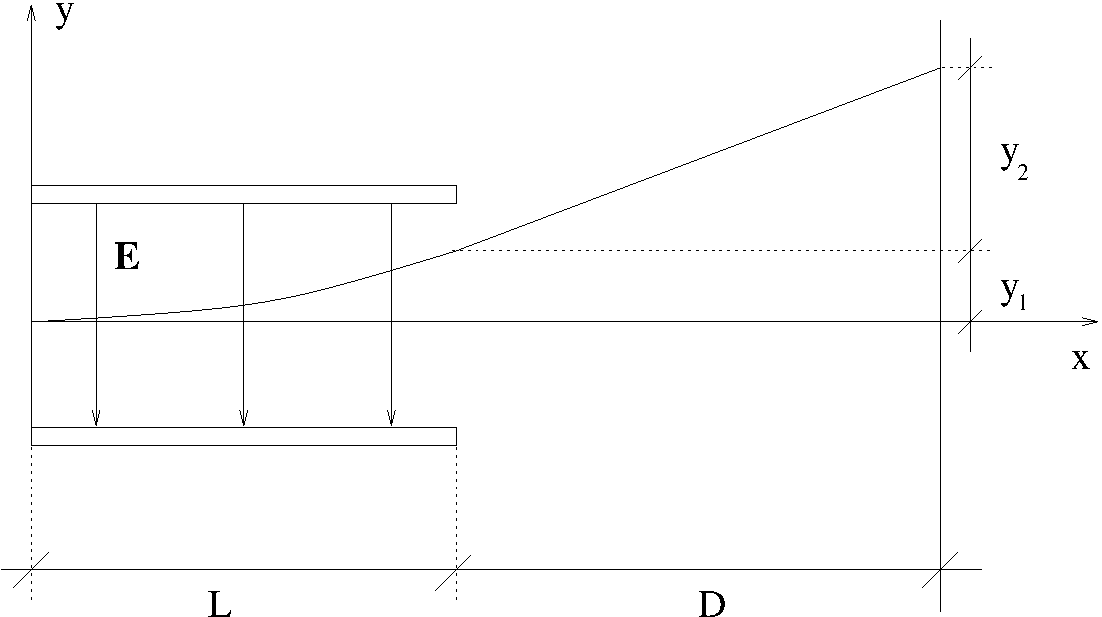
\includegraphics[scale=0.5]{immagini/fisica3/thomson01}
\end{figure}
Applicando solo il campo elettrico:
\begin{equation}
	\ve r=\frac{q\ve E}{2m}t^2+\ve v_0 t
\end{equation}
essendo
\[\ve E=-E\ver \jmath\qquad \ve v_0=v_0\ver \imath\]
\begin{equation}
	\left\{
	\begin{array}{l}
		x=v_0t \\
		y=-\dfrac{qE}{2m}t^2
	\end{array}
	\right.
\end{equation}
eliminando il tempo:
\begin{equation}
	y_1=y(L)=\left.-\frac{qE}{2m}\frac{x^2}{v_0^2}\right|_{x=L}=-\frac{qE}{2m}\frac{L^2}{v_0^2}
\end{equation}
le velocità invece:
\begin{equation}
	\left\{
	\begin{array}{l}
		v_x=v_0 \\
		v_y=-\dfrac{qE}{m}t
	\end{array}
	\right.
\end{equation}
eliminando il tempo:
\begin{equation}
	v_y(L)=\left.-\dfrac{qE}{m}\frac{x}{v_0}\right|_{x=L}=-\dfrac{qE}{m}\frac{L}{v_0}
\end{equation}
Dopo il condensatore si muove di moto rettilineo uniforme:
\begin{equation}
	\left\{
	\begin{array}{l}
		x=L+v_xt=L+v_0t \\
		y=y_2+v_yt=y_2-\frac{qE}{m}\frac{L}{v_0}t
	\end{array}
	\right.
\end{equation}
eliminando il tempo:
\begin{equation}
	y=\left. y_2-\frac{qE}{m}\frac{L}{v_0}\left(\frac{x-L}{v_0}\right)\right|_{L+D}=-\frac{qE}{2m}\frac{L^2}{v_0^2}-\frac{qE}{m}\frac{DL}{v_0^2}=-\frac{qEL}{mv_0^2}\left(\frac{L}{2}+D\right)
	\label{thomson04}
\end{equation}
In questo modo si potrebbe conoscere $\frac{q}{m}$ per inversione. Il problema è che non si conosce $v_0$. Questa grandezza potrebbe essere calcolata sapendo la differenza di potenziale tra il catodo e l'anodo e la loro distanza. Infatti la forza d'accelerazione impressa è pari al potenziale per la distanza per la carica. Thomson invece usò il metodo del separatore di velocità (vedi esempio \ref{spettrometro01} a pag.\@ \pageref{spettrometro01}): si usa un campo magnetico $\ve B=B\ver k$ ortogonale al campo elettrico e si regola l'intensità fino a quando il campo magnetico annulla l'effetto del campo elettrico e i raggi non vengono deviati. In queste condizioni:
\begin{equation}
	\ve F=q\ve E^\star+q\ve v_0\times\ve B^\star=q\left(E^\star+v_0 B^\star\right)\ver \imath=0
\end{equation}
cioè:
\begin{equation}
	v_0=\frac{E^\star}{B^\star}
	\label{velocita_iniziale02}
\end{equation}
L'esperimento è diviso in due parti, nella prima si determina la velocità $\ve v_0$ delle particelle dei raggi catodici usando un campo elettrico $\ve E^\star$ e uno magnetico $\ve B^\star$. Nella seconda parte si applica solo un campo elettrico $\ve E$ e si misura lo spostamento verticale $y$. Sostituendo la \eqref{velocita_iniziale02} nella \eqref{thomson04} si ottiene:
\begin{equation}
	\frac{q}{m}=-\frac{y}{EL(L+2D)}\left(\frac{E^\star}{B^\star}\right)^2
\end{equation}
spesso si usa $E=E^\star$, quindi:
\begin{equation}
	\frac{q}{m}=-\frac{y}{L(L+2D)}\frac{E}{\left(B^\star\right)^2}
\end{equation}
che corrisponde a circa $-\SI{1.758}{\coulomb\per\kilogram}$.
\section{Esperimento di Millikan\index{Millikan}\index{esperimento!di Millikan}}
L'esperimenti do Millikan dimostra che la carica è quantizzata e ne trova il valore minimo. Si consideri la caduta di una goccia d'olio supposta sferica nell'aria. Le forze agenti sono la gravità, la spinta di Archimede e la forza di Stokes:
\begin{equation}
	\ve F=m\ve g-\rho_\text{aria}V\ve g-\beta\ve v
	\label{forze_Millikan}
\end{equation}
con $m$ la massa della goccia, $\rho_\text{aria}$ la densità dell'aria, $\beta$ il coefficiente della forza di Stokes. Prendiamo come positivo l'asse verticale verso il basso. Per una sfera:
\begin{equation}
	\beta=6\pi\eta r
	\label{beta_r}
\end{equation}
con $\eta$ il coefficiente di viscosità dell'aria e $r$ il raggio della goccia, $\eta$ è conosciuto. Innanzitutto vogliamo conoscere $\beta$ e quindi il raggio $r$. La velocità di regime $v_a$ si raggiunge quando la somma delle forze è nulla:
\begin{equation}
	v_a=\frac{m-V\rho_\text{aria}}{\beta}g
	\label{va11}
\end{equation}
questa può essere misurata, infatti dopo qualche costante di tempo $\tau=\frac{m}{\beta}$ si può considerare che la velocità raggiunta sia quella di regime\footnote{risolvendo l'equazione differenziale \eqref{forze_Millikan} in funzione della velocità si trova:
\[
	v(t)=\frac{m-V\rho_\text{aria}}{\beta}g\left(1-e^{-\frac{\beta t}{m}}\right)\xrightarrow{t\to +\infty} v_a
\]
e allora:
\[
	\frac{v(5\tau)-v_a}{v_a}=-e^{-5}\simeq -0,67\%
\]
}.
Sostituendo nella \eqref{forze_Millikan} le espressioni della massa in funzione del volume e l'espressione di $\beta$ e usando la velocità di regime:
\begin{equation}
	\frac{4}{3}\pi r^3\rho_{\text{olio}}g-\rho_\text{aria}\frac{4}{3}\pi r^3 g-6\pi\eta r v_a=0
\end{equation}
possiamo trovare $r$:
\begin{equation}
	r=3\sqrt{\frac{\eta v_a}{2g\left(\rho_\text{olio}-\rho_\text{aria}\right)}}
	\label{va14}
\end{equation}
tornando a $\beta$
\begin{equation}
	\beta=6\pi\eta r=18\pi\sqrt{\frac{\eta^3 v_a}{2 g\left(\rho_\text{olio}-\rho_\text{aria}\right)}}
	\label{va15}
\end{equation}
Il procedimento un po' contorto è la prima parte dell'esperimento che ci consente di trovare $\beta$ a partire da grandezze direttamente misurabili.

La goccia d'olio continuando a cadere entra in un condensatore a facce piane e parallele all'interno del quale è presente un campo elettrico uniforme verticale. La goccia si carica elettricamente per sfregamento con l'aria, con l'ugello, o con una sorgente radioattiva posta nelle sue vicinanze. Assumendo che la goccia sia carica negativamente (potrebbe essere anche carica positivamente) e che il campo elettrico sia tale da imprimere una forza verso il basso si ha:
\begin{equation}
	F=mg-\beta v-\rho_\text{aria}Vg+qE
\end{equation}
si arriverà ad una velocità di regime $v_e\neq v_a$:
\begin{equation}
	\beta v_e=mg-\rho_\text{aria}Vg+qE
\end{equation}
il termine $mg-\rho_\text{aria}Vg$ lo possiamo ricavare dalla \eqref{va11}\footnote{più lineare, ma più lungo sarebbe stato sostituire il valore di $\beta$ in funzione di $v_a$ e $m$ in funzione del raggio $r$ e quest'ultimo in funzione di $v_a$}:
\begin{equation}
	\beta v_e=v_a\beta+qE
\end{equation}
essendo $E$ noto, possiamo ricavare la carica della goccia d'olio:
\begin{equation}
	q=\frac{\beta}{E}(v_e-v_a)=-\frac{18}{\pi}\sqrt{\frac{\eta^3v_a}{2g\left(\rho_\text{olio}-\rho_\text{aria}\right)}}\left(v_a-v_e\right)
\end{equation}
Naturalmente il tutto può essere fatto usando il campo elettrico al contrario o usando gocce di altro materiale, come mercurio\footnote{il problema principale è l'evaporazione}. Osservando le gocce con un microscopio quello che si trova è che la carica delle gocce d'olio è quantizzata e il valore tra le cariche è costante e si suppone essere quello della carica dell'elettrone. Il valore di Millikan era leggermente sbagliato perché usava una sottostima di $\eta$ per l'aria.

\section{Isotopi}
Dopo la scoperta dell'elettrone ci si chiedeva se poteva esistere un flusso di cariche positive che generasse una corrente. La ricerca di queste particelle fu condotta usando un apparato simile a quello per lo studio dei raggi catodici. Goldstein osservò che se nel catodo di un tubo con gas rarefatto aveva una sottile fenditura apparivano raggi luminosi nel gas dalla parte opposta dell'anodo. Questi raggi furono chiamati ``raggi positivi''.

Thomson misurò il rapporto $\frac{q}{m}$. La scarica avveniva in un grande bulbo mantenuto a bassa pressione tra un anodo e un catodo. Il catodo aveva una fenditura, in modo tale che alcuni raggi potevano attraversarlo. Al dì là del catodo si trovavano i poli di un elettromagnete che generavano un campo magnetico $\ve B$, allo stesso tempo era generato un campo elettrico $\ve E$ antiparallelo a $\ve B$. Dopo questa regione di lunghezza $L$ si trova uno spazio di lunghezza $D$ in cui i raggi proseguono in linea retta, prima di arrivare su uno schermo rilevatore.

I raggi arrivano nella regione dei campi con una velocità $\ve v_0=v_{0x}\ver \imath$, in quanto la fenditura fa si che solo la componente $x$ sopravviva. Il campo elettrico sia orientato verso il basso: $\ve E=-E\ver \jmath$ e il campo magnetico verso l'alto: $\ve B=B\ver \jmath$. Le forze che agiscono sui raggi supposti come flusso di particelle cariche sono:
\begin{equation}
	\ve F_E=q\ve E=-qE\ver \jmath\\
\end{equation}
\begin{equation}
	\begin{split}
		\ve F_B&=q\ve v\times\ve B=qB\ve v\times\ver \jmath\\
		&=qB\left(\left(v_y 0-v_z 1\right)\ver \imath+\left(v_z 0-v_x 0\right)\ver \jmath+\left(v_x 1-v_y 0\right)\ver k\right)\\
		&=qB\left(-v_z\ver \imath+v_x\ver k\right)
	\end{split}
\end{equation}
Notiamo che la forza elettrica modifica solo la $v_y$ che non influenza la $\ve F_B$, quindi potremmo usare semplicemente i procedimenti fatti precedentemente. Impostando il problema di Cauchy usando il formalismo newtoniano $m\ddot{\ve r}=\ve F$:
\begin{equation}
	\left\{
	\begin{aligned}
		m\ddot x & =-qB\dot z \\
		m\ddot y & =-qE       \\
		m\ddot z & =qB\dot x
	\end{aligned}
	\right.
	\qquad
	\left\{
	\begin{aligned}
		x(0)      & =0      \\
		y(0)      & =0      \\
		z(0)      & =0      \\
		\dot x(0) & =v_{0x} \\
		\dot y(0) & =0      \\
		\dot z(0) & =0      \\
	\end{aligned}
	\right.
\end{equation}
La seconda equazione è disaccoppiata dalle altre ed è facilmente integrabile:
\begin{equation}
	y(t)=-\frac{1}{2}\frac{qE}{m}t^2
\end{equation}
Per disaccoppiare le rimanenti possiamo derivarle ulteriormente:
\begin{equation}
	\left\{
	\begin{aligned}
		m\dddot x & =-qB\ddot z \\
		m\dddot z & =qB\ddot x
	\end{aligned}
	\right.
\end{equation}
Partiamo dalla seconda, sostituendo $\ddot x$:
\begin{equation}
	\dddot z=\left(\frac{qB}{m}\right)\ddot x=-\left(\frac{qB}{m}\right)^2\dot z
	\label{dddotz}
\end{equation}
che è autonoma, facile da risolvere:
\[
	\lambda^3+\left(\frac{qB}{m}\right)^2\lambda=0\qquad\lambda_1=0\quad\lambda_{2/3}=\pm\frac{qB}{m}i
\]
Allora la soluzione generale è:
\begin{equation}
	z(t)=C_1 e^{\lambda_1t}+C_2 e^{\lambda_2t}+C_3 e^{\lambda_3t}=C_1+C_2\cos\left(\frac{qB}{m}t\right)+C_3\sin\left(\frac{qB}{m}t\right)
	\label{soluzione_generale_EB}
\end{equation}
Troviamo la soluzione generale anche per $x(t)$:
\begin{equation}
	\dddot x=-\left(\frac{qB}{m}\right)\ddot z=-\left(\frac{qB}{m}\right)^2
\end{equation}
che è esattamente la \eqref{dddotz}, quindi la soluzione deve essere del tipo \eqref{soluzione_generale_EB}:
\begin{equation}
	x(t)=C_4+C_5\cos\left(\frac{qB}{m}t\right)+C_6\sin\left(\frac{qB}{m}t\right)
\end{equation}
Iniziamo ad imporre le condizioni iniziali $z(0)=0$:
\begin{equation}
	0=z(0)=C_1+C_2\qquad C_2=-C_1
\end{equation}
e anche per $x$: $C_5=-C_4$. Per le velocità $\dot z(0)=0$:
\begin{equation}
	0=\dot z(0)=C_3\frac{qB}{m}\Rightarrow C_3=0
\end{equation}
mentre per $x$:
\begin{equation}
	v_{0x}=\dot x(0)=C_6\frac{qB}{m}\Rightarrow C_6=v_{0x}\frac{m}{qB}
\end{equation}
Non siamo riusciti a determinare tutte le costanti perché abbiamo solo due condizioni iniziali, mentre stiamo risolvendo un equazione del terz'ordine, le informazioni aggiuntive saranno ricavate dal modo in cui le equazioni differenziali per $x$ e per $z$ sono accoppiate; riassumiamo quello che abbiamo trovato:
\begin{gather}
	z(t)=C_1-C_1\cos\left(\frac{qB}{m}t\right)\\
	x(t)=C_4-C_4\cos\left(\frac{qB}{m}t\right)+v_{0x}\frac{m}{qB}\sin\left(\frac{qB}{m}t\right)
\end{gather}
Usiamo le condizioni di accoppiamento:
\begin{equation}
	\left\{
	\begin{aligned}
		\ddot x & =-\frac{qB}{m}\dot z \\
		\ddot z & =\frac{qB}{m}\dot x  \\
	\end{aligned}
	\right.
\end{equation}
facendo le derivate:
\begin{equation}
	\left\{
	\begin{aligned}
		C_4\frac{qB}{m}\cos\left(\frac{qB}{m}t\right)-v_{0x}\sin\left(\frac{qB}{m}t\right)=-C_1\frac{qB}{m}\sin\left(\frac{qB}{m}t\right) \\
		C_1\frac{qB}{m}\cos\left(\frac{qB}{m}t\right)=C_4\frac{qB}{m}\sin\left(\frac{qB}{m}t\right)+v_{0x}\cos\left(\frac{qB}{m}t\right)
	\end{aligned}
	\right.
\end{equation}
Riscriviamo in questo modo:
\begin{equation}
	\left\{
	\begin{aligned}
		qBC_4\cos\left(\frac{qB}{m}t\right)+\left(qBC_1-v_{0x}m\right)\sin\left(\frac{qB}{m}t\right)=0 \\
		\left(C_1qB+v_{0x}m\right)\cos\left(\frac{qB}{m}\right)-C_4qB\sin\left(\frac{qB}{m}t\right)=0
	\end{aligned}
	\label{sistema_molto_bastardo}
	\right.
\end{equation}
Dividendo:
\begin{equation}
	\frac{qBC_4}{C_1qB+v_{0x}m}=\frac{qBC_1-v_{0x}m}{C_4qB}
\end{equation}
ovvero:
\begin{equation}
	\left(C_1qB+v_{0x}m\right)^2=-\left(qBC_4\right)^2
\end{equation}
che è vera se :
\begin{equation}
	qBC_4=0
\end{equation}
cioè $C_4=0$. Oppure se
\begin{equation}
	C_1qB+v_{0x}m=0
\end{equation}
cioè $C_1=\frac{v_{0x}m}{qB}$
Eguagliando e raccogliendo le equazioni del sistema \eqref{sistema_molto_bastardo}:
\begin{equation}
	\left(qBC_4-C_1qV+v_{0x}m\right)\cos\left(\frac{qB}{m}t\right)+\left(qBC_1-v_{0x}m+C_4qB\right)\sin\left(\frac{qB}{m}t\right)=0
\end{equation}
e sostituendo $C_4=0$ si ottiene $C_1=\frac{v_{0x}m}{qB}$. Allo stesso modo sostituendo $C_1=\frac{v_{0x}m}{qB}$ si ottiene $C_4$=0.
Dopo tutti questi conti le equazioni del moto e le velocità delle particelle all'interno del campo magnetico ed elettrico sono:
\begin{equation}
	\left\{
	\begin{aligned}
		x(t) & =\frac{m}{qB}v_{0x}\sin\left(\frac{qB}{m}t\right)              \\
		y(t) & =-\frac{1}{2}\frac{qE}{m}t^2                                   \\
		z(t) & =\frac{m}{qB}v_x-\frac{m}{qB}v_x\cos\left(\frac{qB}{m}t\right)
	\end{aligned}
	\right.\quad
	\left\{
	\begin{aligned}
		v_x(t) & =v_{0x}\cos\left(\frac{qB}{m}t\right) \\
		v_y(t) & =\frac{qE}{m}t                        \\
		v_z(t) & =v_{0x}\sin\left(\frac{qB}{m}t\right)
	\end{aligned}
	\right.
\end{equation}

\chapter{Radiazione di corpo nero\index{radiazione!di corpo nero}\index{corpo nero}}
\minitoc
\section{Radiazione termica}
Un corpo emette della radiazione visibile se è caldo abbastanza. Possiamo scomporre questa radiazione con un prisma ed analizzarne le componenti, per esempio potremmo mettere in relazione l'emittanza monocromatica $R(\lambda)=\frac{\ud W}{\ud \lambda}$, cioè la potenza irradiata per unità di superficie per la lunghezza d'onda compresa tra $\lambda$ e $\lambda+\ud\lambda$, con $\lambda$. Si osserva che ogni corpo ha la sua curva $R(\lambda)$. Facendo l'inviluppo di tutte le funzioni $R(\lambda)$ variando il tipo di materiale e usando la stessa temperatura si ottiene una curva, quella della radiazione di corpo nero.

Ogni corpo emettere dell'energia per irraggiamento, cioè radiazione, questo fa si che si crei un equilibrio termico tra vari corpi anche senza un contatto. Infatti se il corpo $A$ è più caldo del corpo $B$, ci sarà un flusso netto di radiazione da $A$ a $B$ fino a quando $B$ assorbendo la radiazione di $A$ convertendola in energia interna non avrà la stessa temperatura di $A$ che contemporaneamente si è raffreddato per perdita di energia interna sotto forma di radiazione verso $B$. Aumentando la temperatura di un corpo aumenta la potenza da esso irradiata.

Consideriamo un intervallo di lunghezze d'onda infinitesimo dello spettro di emissione di $n$ corpi opachi in equilibrio termico tra loro e l'ambiente. Poiché i corpi sono opachi non possono trasmettere la radiazione, parte di essa sarà assorbita e parte riflessa. Sia $E$ l'energia che arriva su un corpo. La parte di energia riflessa sarà $aE$, quella riflessa $rE$. $a$ è il coefficiente di assorbimento, $r$ di riflessione. Naturalmente essendo tutta la radiazione o riflessa o assorbita:
\begin{equation}
	E=aE+rE=(a+r)E\quad\Rightarrow \qquad(a+r)=1
\end{equation}
per tutti i corpi $a_1+r_1=1\ldots a_n+r_n=1$. Poiché i corpi sono in equilibrio termico tra di loro e con l'ambiente (li possiamo considerare nel vuoto) l'energia irradiata dal primo corpo in un certo $\Delta t$ deve essere uguale all'energia assorbita:
\begin{equation}
	W_1\Delta A_1\Delta t=a_1I\Delta A_1\Delta t
	\label{emittanza01}
\end{equation}
con $W_1$ l'emittanza, $\Delta A_1$ l'area della superficie e $I$ l'intensità ricevuta dagli altri corpi. Questo vale per tutti i corpi:
\begin{equation}
	W_2\Delta A_2\Delta t=a_2I\Delta A_2\Delta t
	\label{emittanza02}
\end{equation}
Dividendo membro a membro la \eqref{emittanza01} e la \eqref{emittanza02}:
\begin{equation}
	\frac{W_1}{W_2}=\frac{a_1}{a_2}
\end{equation}
o meglio:
\begin{equation}
	\frac{W_1}{a_1}=\frac{W_2}{a_2}
	\label{emittanza03}
\end{equation}
cioè il rapporto $\frac{W}{a}$ è costante per qualsiasi corpo (dipenderà dalla lunghezza d'onda e dalla temperatura). Quindi se un corpo ha un $W$ alto, cioè è un buon emettitore allora avrà un alto valore di $a$ cioè sarà un buon assorbitore.
\section{Corpo nero}
Un corpo nero è un perfetto emettitore, o equivalentemente un perfetto assorbitore. Per un corpo nero $a=1$. Il modo pratico per costruire un corpo nero è quello di usare una cavità con un piccolo foro. Ritornando all'equazione \eqref{emittanza03}:
\begin{legge}[Kirchhoff\index{legge!di Kirchhoff}\index{Kirchhoff}]
	Ad una data temperatura
	\begin{equation}
		\frac{W_1}{a_1}=\frac{W_2}{a_2}=\frac{W_b}{1}=W_b
	\end{equation}
	con $W_b$ l'emittanza del corpo nero.
\end{legge}
Quindi il rapporto tra l'emittanza e il coefficiente di assorbimento è pari all'emittanza del corpo nero.
\subsection{Legge Stefan--Boltzmann}
La potenza per unità di area emessa dal corpo nero $W_b$ è data dall'integrale della curva $R(\lambda)$ su $\field{R}^+$. Stefen trovò empiricamente:
\begin{legge}[Stefan--Boltzmann]
	\begin{equation}
		W_b=\sigma T^4
	\end{equation}
\end{legge}
con $\sigma$ costante di Stefan--Boltzmann. La legge empirica di Stefan era stata derivata teoricamente da Boltzmann. Per un corpo generico possiamo dire:
\begin{equation}
	W=aW_b=a\sigma T^4
\end{equation}
\subsection{Legge di Wien}
Cambiando temperatura la funzione $R(\lambda)$ cambia e in particolare cambia il massimo. Si nota che rimane costante:
\begin{legge}[legge di Wien]
	\begin{equation}
		\lambda_\text{max}T = \const
	\end{equation}
\end{legge}
\subsection{Cavità}
Dimostriamo che una cavità con un piccolo foro si comporta come un corpo nero, ciò vorrà dire che è solo la geometria che importa. Consideriamo due pareti, una di fronte all'altra, contenute in un contenitore che le isola dall'esterno. Su una delle due pareti sia praticato un foro molto piccolo rispetto all'area della parete. Consideriamo un intervallo di tempo $\Delta t$. La parete $A$ emette una certa energia per unità di area pari a $W_A\Delta t$ (anche in assenza della seconda parete), questa arriva sulla seconda parete, ed è riflessa parzialmente, esattamente $r_BW_A\Delta t=(1-a_B)W_A\Delta t$, quest'energia arriva sulla parete indietro che riflette $(1-a_A)(1-a_B)W_A\Delta t$, eccetera. Lo stesso discorso si può fare per l'energia che parte dalla parete $B$. Riassumiamo:
\begin{equation}
	\begin{array}{cl|cl}
		\rightarrow & W_A\Delta t                   & \leftarrow  & W_B\Delta t                   \\
		\leftarrow  & (1-a_B)W_A\Delta t            & \rightarrow & (1-a_A)W_B\Delta t            \\
		\rightarrow & (1-a_A)(1-a_B)W_A\Delta t     & \leftarrow  & (1-a_A)(1-a_B)W_B\Delta t     \\
		\leftarrow  & (1-a_A)(1-a_B)^2W_A\Delta t   & \rightarrow & (1-a_A)^2(1-a_B)W_B\Delta t   \\
		\rightarrow & (1-a_A)^2(1-a_B)^2W_A\Delta t & \leftarrow  & (1-a_A)^2(1-a_B)^2W_B\Delta t \\
		\leftarrow  & (1-a_A)^2(1-a_B)^3W_A\Delta t & \rightarrow & (1-a_A)^3(1-a_B)^2W_B\Delta t \\
		\ldots      & \ldots                        & \ldots      & \ldots                        \\
	\end{array}
\end{equation}
Supponiamo che il nostro piccolo foro sia praticato nella parete di destra, quindi l'energia per area $W_r$ che uscirà sarà la somma di tutte le riflessioni verso destra $\rightarrow$:
\begin{multline}
	W_r\Delta t=W_A\Delta t+(1-a_A)(1-a_B)W_A\Delta t+(1-a_A)^2(a-a_B)^2W_A\Delta t+\ldots+\\+(1-a_A)W_B\Delta t+(1-a_A)^2(1-a_B)W_B\Delta t+(1-a_A)^3(1-a_B)^2\Delta t+\ldots
\end{multline}
che è la somma di due serie geometriche:
\begin{equation}
	\begin{split}
		W_r&=W_A\sum_{n=0}^\infty\left[(1-a_A)(1-a_B)\right]^n+W_B(1-a_A)\sum_{n=0}^\infty\left[(1-a_A)(1-a_B)\right]^n\\
		&=\left(W_A+W_B\left(1-a_A\right)\right)\sum_{n=0}^\infty\left[(1-a_A)(1-a_B)\right]^n\\
		&=\left(W_A+W_B\left(1-a_A\right)\right)\frac{1}{1-(1-a_A)(1-a_B)}\\
		&=\left(a_AW_b+a_BW_b(1-a_A)\right)\frac{1}{a_A+a_B-a_Aa_B}\\
		&=W_b\frac{a_A+a_B+a_Aa_B}{a_A+a_B+a_Aa_B}=W_b
	\end{split}
\end{equation}
avendo ricordato che
\[
	W_A=a_AW_b\quad W_B=a_BW_b
\]
con $W_b$ la radiazione del corpo nero e una nota relazione algebrica\footnote{serie geometrica:
	\begin{equation}
		\begin{split}
			\sum_{k=0}^\infty x^k&=\lim_{n\to\infty}\sum_{k=0}^n x^k=\lim_{n\to\infty}\left(1+x+x^2+x^3+\ldots+x^n\right)\\
			&=\lim_{n\to\infty}\frac{1}{1-x}\left((1-x)+(1-x)x+(1-x)x^2+(1-x)x^3+\ldots+(1-x)x^n\right)\\
			&=\lim_{n\to\infty}
			\left\{
			\begin{array}{ll}
				\dfrac{1-x^{n+1}}{1-x} & x\neq 1 \\
				n+1                    & x=1
			\end{array}
			\right.=
			\left\{
			\begin{array}{ll}
				\dfrac{1}{1-x} & |x|<1    \\
				+\infty        & x\geq 1  \\
				\nexists       & x\leq -1
			\end{array}
			\right.
		\end{split}
	\end{equation}
	Nel nostro caso $x=(1-a_A)(1-a_B)$ $0<x<1$
}. Abbiamo allora dimostrato che la radianza che esce dalla fenditura nella cavità è proprio quella del corpo nero. Questo è di fondamenta importanza, oltre a permetterci di costruire un corpo nero come cavità, questa affermazione dice che per studiare la radiazione di corpo nero possiamo studiare la radiazione all'interno di una cavità.
\subsection{Wien}
Wien notò la somiglianza della curva $R(\lambda)$ che descrive la potenza per unità di area per una lunghezza d'onda compresa tra $(\lambda,\lambda+\ud\lambda)$ con la distribuzione di Maxwell per le velocità. Usando questo tipo di funzione e cercando i coefficienti che interpolassero i dati ottenne:
\begin{equation}
	R(\lambda)=\frac{c_1\lambda^{-5}}{e^{\frac{c_2}{\lambda T}}}
\end{equation}
$c_1$ e $c_2$ sono chiamati prima e seconda costante di radiazione.
\section{Radiazione della cavità}
Come abbiamo detto la radiazione di un corpo nero è uguale alla radiazione emessa da un corpo nero. Studiamo quindi lo spettro della densità di energia della radiazione all'interno di una cavità $\rho$. Questa quantità non è altro che l'energia per unità di volume all'interno della cavità nell'intervallo di frequenze (o lunghezze d'onda corrispondenti) $\nu$-$\nu+\ud\nu$. È evidente che:
\begin{equation}
	\rho \propto R
\end{equation}

\section{Rayleigh--Jeans}
Un modo rigoroso è quello intrapreso da Lord Rayleigh. Egli suppone che nella cavità le onde stazionarie abbiano l'energia $kT$ somma dell'energia cinetica su un grado di libertà e di quella potenziale. Ogni onda stazionaria ha un certo numero di modi di oscillare, ognuno dei quali ha energia $kT$.
\subsection{Modi di oscillare}
Un'onda monodimensionale stazionaria è tale che:
\begin{equation}
	L=n\frac{\lambda}{2}
\end{equation}
con $n$ naturale. Consideriamo $\lambda\ll L$. Differenziando:
\begin{equation}
	\ud n=-\frac{2}{\lambda^2}L\ud \lambda
\end{equation}
\begin{Es}[numero di modi di oscillare]
	Se una corda è lunga $L=\SI{1}{\meter}$ e l'intervallo di lunghezze d'onda è $(\lambda,\lambda+\Delta\lambda)=(\SI{1}{\centi\meter},\SI{1.1}{\centi\meter})$ allora ci sono:
	\[
		\Delta n=\frac{2L}{\lambda^2}\Delta\lambda=\frac{2\cdot\SI{1}{\meter}}{(\SI{0.01}{\meter})^2}\,\SI{0.001}{\meter}=20
	\]
	modi di oscillare.

	Se avessimo fatto un conto esatto allora:
	\[
		\Delta n=n_2-n_1=2L\left(\frac{1}{\lambda_2}-\frac{1}{\lambda_1}\right)\simeq 18.1
	\]
	quindi contando anche gli estremi ci sono 19 modi di oscillare.
\end{Es}

Passiamo al problema tridimensionale. Ipotizziamo che la cavità si cubica di lato $L$. L'onda stazionaria che si propaga sarà del tipo:
\begin{equation}
	E_x=E_0\cos(k_x x)\sin(k_y y)\sin(k_z z)\sin\omega t
\end{equation}
e così per le altre componenti. La condizione al contorno che deve rispettare è che le componenti parallele a ogni superficie devono essere nulle sulla superficie (la stessa cosa avveniva per il caso monodimensionale). Per esempio consideriamo la parete $y=L$, qui deve valere:
\begin{equation}
	\left\{
	\begin{array}{l}
		E_x(x,L,z)=E_0\cos(k_x x)\sin(k_y L)\sin(k_z z)\sin\omega t=0 \\
		E_z(x,L,z)=E_0\cos(k_z z)\sin(k_y L)\sin(k_x x)\sin\omega t=0 \\
	\end{array}
	\right.\qquad
	k_y L=n_y\pi
\end{equation}
e così via con $n_x,n_y,n_z\in\field{N}$.
\begin{equation}
	\omega=\norm{\ve k}c=\frac{\pi c}{L}\left(n_x^2+n_y^2+n_z^2\right)^{\frac{1}{2}}
\end{equation}
fissato $\omega$ il vettore $\ve n$ ha modulo:
\begin{equation}
	\norm{\ve n}=\frac{\omega L}{\pi c}
	\label{contorno3Dstaz}
\end{equation}
Vogliamo sapere quanti modi di oscillare con pulsazione minore di $\omega$. Per ogni scelta di $\ve n$ ci sono 2 modi di oscillare dati dalla polarizzazione. Quindi il numero di modi di oscillare è:
\begin{equation}
	2\frac{1}{8}\frac{4}{3}\pi\left(\frac{\omega L}{\pi c}\right)^3=\frac{\omega^3 V}{3\pi^2 c^3}=\frac{8\pi V}{3\lambda^3}
\end{equation}
Il $2$ deriva dal fatto che per ogni scelta di $\ve n$ ci sono 2 polarizzazioni, mentre l'ottavo deriva dal fatto che le componenti di $\ve n$ possono essere solo positive. Differenziando come prima possiamo sapere quanti modi di oscillare ci sono per lunghezze d'onda comprese tra $(\lambda,\lambda+\ud\lambda)$:
\begin{equation}
	\ud N=\frac{8\pi V}{\lambda^4}\,\ud\lambda
	\label{numero modi di oscillare 3d}
\end{equation}

\subsection{Legge di Rayleigh--Jeans}
Dall'equazione \eqref{numero modi di oscillare 3d} divisa per $V$ otteniamo la densità di modi. Associando ad ogni modo l'energia $kT$ si ottiene:
\begin{equation}
	R(\lambda)=\frac{8\pi kT}{\lambda^4}
\end{equation}
Che è la potenza monocromatica per unità di area secondo Rayleigh--Jean. Questa funzione per $\lambda\to 0$ tende a $+\infty$, che è ovviamente impossible, la cosidetta catastrofe ultravioletta. Dalla legge di Rayleigh--Jeans si deduce che la fisica classica non è capace di descrivere lo spettro del corpo nero.
\section{Planck\index{Planck}}
Planck postula che l'energia degli oscillatori sia discreta, multipla intera di $\epsilon$. Il numero di oscillatori aventi l'energia $m\epsilon$ con $m \in \field{N}$ è:
\begin{equation}
	n_m=n_0e^{-\frac{E_m}{kT}}=n_0e^{-\frac{m\epsilon}{kT}}
\end{equation}
e la loro energia totale:
\begin{equation}
	E_{m\epsilon}=n_m (m\epsilon)=m\epsilon n_0e^{-\frac{m\epsilon}{kT}}
\end{equation}
il numero totale di particelle:
\begin{equation}
	N=\sum_{m=0}^\infty n_m=\sum_{m=0}^\infty n_0e^{-\frac{m\epsilon}{kT}}=n_0\sum_{m=0}^\infty \left(e^{-\frac{\epsilon}{kT}}\right)^m=n_0\frac{1}{1-e^{-\frac{\epsilon}{kT}}}
\end{equation}
essendo una serie geometrica di ragione $0<e^{-\frac{\epsilon}{kT}}<1$. L'energia media sarà\footnote{ricordiamo lo sviluppo in serie di $(1-x)^{-2}$:
	\[
		\left(1-x\right)^{-2}=\sum_{m=0}^{\infty}(m+1)x^m=\sum_{m=1}^\infty m x^{m-1}
	\]
} allora:
\begin{equation}
	\begin{split}
		\media{E}&=\sum_{m=0}^\infty \frac{E_{m\epsilon}}{N}=\sum_{m=0}^\infty\frac{m\epsilon n_0e^{-\frac{m\epsilon}{kT}}}{n_0\frac{1}{1-e^{-\frac{\epsilon}{kT}}}}=\epsilon\sum_{m=1}^\infty\frac{m \left(e^{-\frac{\epsilon}{kT}}\right)^m}{\frac{1}{1-e^{-\frac{\epsilon}{kT}}}}\\
		&=\epsilon e^{-\frac{\epsilon}{kT}}\frac{\sum_{m=1}^\infty m \left(e^{-\frac{\epsilon}{kT}}\right)^{m-1}}{\left(1-e^{-\frac{\epsilon}{kT}}\right)^{-1}}
		=\epsilon e^{\frac{-\epsilon}{kT}}\dfrac{\left(1-e^{\frac{-\epsilon}{kT}}\right)^{-2}}{\left(1-e^{-\frac{\epsilon}{kT}}\right)^{-1}}=\epsilon e^{\frac{-\epsilon}{kT}}\frac{1}{1-e^{-\frac{\epsilon}{kT}}}=\frac{\epsilon}{e^{\frac{\epsilon}{kT}}-1}
	\end{split}
	\label{energia Planck modi01}
\end{equation}
La densità di modi di oscillare è data dalla \eqref{numero modi di oscillare 3d} divisa per il volume, quindi la potenza per unità di area totale, associando ad ogni modi di oscillare la \eqref{energia Planck modi01}, è:
\begin{equation}
	R(\lambda)=\frac{8\pi}{\lambda^4}\frac{\epsilon}{e^\frac{\epsilon}{kT}-1}
\end{equation}
per tornare al caso classico dobbiamo ammettere che l'energia non sia quantizzata, cioè $\epsilon\to 0$
\begin{equation}
	\media{E_\text{classico}}=\lim_{\epsilon\to 0} \media{E}=\lim_{\epsilon\to 0}\frac{\epsilon}{e^{\frac{\epsilon}{kT}}-1}=\lim_{\epsilon\to 0}\frac{\epsilon}{\frac{\epsilon}{kT}}=kT
\end{equation}
l'energia $\epsilon$ non è costante ma varia con la frequenza:
\begin{equation}
	\epsilon=h\nu=\frac{hc}{\lambda}
\end{equation}
con $h$ costante di Planck\index{costante!di Planck}. La distribuzione della radianza diventa:
\begin{equation}
	R(\lambda)=\frac{8\pi}{\lambda^5}\frac{hc}{e^\frac{hc}{\lambda kT}-1}
\end{equation}
questa distribuzione si adegua bene ai dati sperimentali, evitando la catastrofe ultravioletta ad alte frequenze, infatti ad alte frequenze $\epsilon$ è molto grande e la probabilità che un modo di oscillare con quella frequenza esista è molto bassa.

Il fatto che l'energia è quantizzata significa anche che l'emissione di energia da parte del corpo nero è quantizzata, cioè sotto forma di quanti\index{quanti} o fotoni\index{fotoni}, ognuno dei quali trasporta energia $h\nu$.






\chapter{Calore specifico dei solidi\index{calore specifico!dei solidi|(}}
\minitoc
Consideriamo trasformazioni a volume costante, queste trasformazioni hanno il vantaggio di compiere lavoro nullo, infatti $\delta L=-p\ud V$; per il primo principio della termodinamica:
\begin{equation}
	\ud U=\delta Q+\delta L
\end{equation}
con $U$ l'energia interna di un sistema che diventa
\begin{equation}
	\ud U=\delta Q
	\label{volume_costante11}
\end{equation}
il calore in relazione al calore specifico molare, in questo caso a volume costante è:
\begin{equation}
	\delta Q=nc_V\ud T
\end{equation}
ma per la \eqref{volume_costante11}:
\begin{equation}
	c_v=\frac{1}{n}\frac{\ud U}{\ud T}
\end{equation}
spesso lavoreremo considerando un solo atomo o una sola mole.
\section{Doulong--Petit}
Se la temperatura di un gas è una misura diretta dell'energia cinetica traslazionale delle sue molecole la temperatura di un solido è la misura dell'energia cinetica degli atomi che vibrano attorno alle loro posizione di equilibrio nel reticolo. Se un solido e un gas sono in equilibrio termico significa che hanno la stessa temperatura e quindi la stessa energia cinetica media $\frac{3}{2}kT$ per atomo. Se immaginiamo ogni atomo come un oscillatore armonico, l'energia potenziale sarà:
\begin{equation}
	V=\frac{1}{2}\beta x^2
\end{equation}
dato che l'equazione del moto armonico, considerando come condizioni iniziale $x=0$ e velocità massima:
\begin{gather}
	x(t)=A\sin\left(\sqrt{\frac{\beta}{m}}t\right)\\
	\dot x(t)=A\sqrt{\frac{\beta}{m}}\cos\left(\sqrt{\frac{\beta}{m}}t\right)
\end{gather}
possiamo ricavare come variano $E_C$ e $U$:
\begin{gather}
	E_C(t)=\frac{1}{2}mv^2=\frac{1}{2}{A^2\beta}\cos^2\left(\sqrt{\frac{\beta}{m}}t\right)\\
	U(t)=\frac{1}{2}\beta x^2=\frac{1}{2}A^2 \beta\sin^2\left(\sqrt{\frac{\beta}{m}}t\right)
\end{gather}
calcoliamo i valori medi:
\begin{gather}
	\media{E_C}=\frac{1}{\pi\sqrt{\frac{m}{\beta}}}\int_0^{\pi\sqrt{\frac{m}{\beta}}} E_c(t)\ud t=\frac{A^2\beta}{4}\\
	\media{U}=\frac{1}{\pi\sqrt{\frac{m}{\beta}}}\int_0^{\pi\sqrt{\frac{m}{\beta}}} U(t)\ud t=\frac{A^2\beta}{4}
\end{gather}
il calcolo non era necessario in quanto $U(t)$ e $E_C(t)$ sono due funzioni uguali, ma sfasate, quindi in un periodo l'area sottesa sottesa deve essere uguale. Concludiamo che l'energia cinetica media per atomo e l'energia potenziale cinetica per atomo sono uguali.
Sommando l'energia cinetica ($\frac{3}{2}kT$) e quella potenziale l'energia media per atomo diventa:
\begin{equation}
	E_\text{atomo}=3kT
\end{equation}
e per una mole:
\begin{equation}
	E=3kN_AT=3RT
\end{equation}
Allora possiamo calcolare il calore specifico a volume costante:
\begin{equation}
	c_v=\frac{\ud E}{\ud T}=3R\simeq \SI{24.94}{\joule\per\mole\per\kelvin}
\end{equation}
che è la legge di Doulon--Petit\index{Doulong}\index{Petit}\index{legge!Doulong--Petit}. Nella semplice derivazione non abbiamo tenuto conto dei possibili cambiamenti della struttura cristallina e dell'energia associata agli elettroni liberi (nei metalli). I dati sperimentali mostrano che la legge di Doulong--Petit funziona solo per temperature molto alte e vale per tutti i materiali solidi. Il teorema di equipartizione dell'energia fallisce.
\section{Einstein\index{Einstein}}
Nel 1906 Einstein derivò il calore specifico dei solidi assumendo ipotesi simili a quelle di Planck per la radiazione di corpo nero. Assumiamo che il nostro solido contenga $N$ atomi, e possa essere rappresentato come $3N$ oscillatori. Il modello di Eintein si caratterizza per associare ad ogni oscillatore la stessa frequenza $\nu$ uguale per tutti. In accordo con Planck l'energia di un oscillatore può essere\footnote{in realtà sarebbe più corretto\[\epsilon_n=\left(n+\frac{1}{2}\right)h\nu\]}:
\begin{equation}
	\epsilon_n=nh\nu\quad n\in\field{N}
\end{equation}
L'energia media risulta allora:
\begin{equation}
	\media{\epsilon}=\dfrac{\sum_{n=0}^{\infty}\epsilon e^{-\frac{\epsilon}{kT}}}{\sum_{n=0}^\infty e^{-\frac{\epsilon}{kT}}}=\dfrac{\sum_{n=0}^{\infty}nh\nu e^{-\frac{nh\nu}{kT}}}{\sum_{n=0}^\infty e^{-\frac{nh\nu}{kT}}}
\end{equation}
per valutare questa serie possiamo usare lo stesso procedimento che abbiamo usato per Planck, nell'equazione \eqref{energia Planck modi01}. Infatti il denominatore è una serie geometrica di ragione $e^{-\frac{h\nu}{kT}}$; il numeratore invece dopo gli opportuni raccogliamenti è lo sviluppo in serie di $\frac{1}{(1-e^{-\frac{h\nu}{kT}})^2}$:
\begin{equation}
	\media{\epsilon}=\dfrac{h\nu}{e^{\frac{h\nu}{kT}}-1}
\end{equation}
che contempla il risultato classico, per alte temperature:
\begin{equation}
	\media{\epsilon_\text{classico}}=\lim_{T\to\infty}\media{\epsilon}=\lim_{T\to\infty}\dfrac{h\nu}{e^{\frac{h\nu}{kT}}-1}=\frac{h\nu}{\frac{h\nu}{kT}}=kT
\end{equation}
L'energia di tutto il solido:
\begin{equation}
	E=3N\media{\epsilon}=3N\dfrac{h\nu}{e^{\frac{h\nu}{kT}}-1}
\end{equation}
e il calore specifico:
\begin{equation}
	\begin{split}
		c_V=&\frac{1}{n}\frac{\partial}{\partial T}E=\frac{1}{n}\frac{\partial}{\partial T}3N\dfrac{h\nu}{e^{\frac{h\nu}{kT}}-1}=
		\frac{3N}{n}\frac{(h\nu)^2}{kT^2}\frac{e^{\frac{h\nu}{kT}}}{\left(e^{\frac{h\nu}{kT}}-1\right)^2}\\=&3R\left(\frac{h\nu}{kT}\right)^2\dfrac{e^{\frac{h\nu}{kT}}}{\left(e^{\frac{h\nu}{kT}}-1\right)^2}
	\end{split}
	\label{cv_einstein01}
\end{equation}
Tanto quanto l'energia media $\media{\epsilon}$ tende a quella classica per $T\to\infty$ anche il calore specifico di Einstein tende al calore specifico di Doulong--Petit:
\begin{equation}
	\lim_{T\to\infty} c_V=\lim_{T\to\infty}3R\left(\frac{h\nu}{kT}\right)^2\dfrac{e^{\frac{h\nu}{kT}}}{\left(e^{\frac{h\nu}{kT}}-1\right)^2}=3R
\end{equation}
Introduciamo la temperatura di Einstein $\Theta_E$:
\begin{equation}
	\Theta_E=\frac{h\nu}{k}
\end{equation}
che ha proprio le dimensioni di una temperatura. Il calore specifico \eqref{cv_einstein01} si può scrivere:
\begin{equation}
	c_v=3R\left(\frac{\Theta_E}{T}\right)^2\dfrac{e^{\frac{\Theta_E}{T}}}{\left(e^{\frac{\Theta_E}{T}}-1\right)^2}
\end{equation}
questa espressione va a zero come $e^{-\frac{\Theta_E}{T}}$. Sperimentalmente si nota invece che i calori specifici vanno a zero come $T^3$. In pratica il calore specifico diminuisce troppo rapidamente a basse temperature.
\section{Debye\index{Debye}}
\subsection{Modi di vibrare in un cristallo}
Ripartiamo da quello che avevamo detto per la cavità. La condizione al contorno che l'onda stazionaria tridimensionale deve soddifare è la \eqref{contorno3Dstaz}:
\begin{equation}
	\norm{\ve n}=\frac{\omega L}{\pi c_S}=\frac{2\pi\nu L}{\pi c_S}=\frac{2\nu L}{c_S}
	\label{nnn01}
\end{equation}
dove $c$ è stato sostituito con $c_S$ essendo ora non più onde elettromagnetiche, ma onde meccaniche. I modi di vibrare compresi tra $n$ e $n+\ud n$ sono:
\begin{equation}
	\ud N=\frac{1}{8}4\pi n^2\ud n=2\pi \frac{\nu^2 L^2}{c_S^2}\ud n
	\label{udN01}
\end{equation}
che è il volume di una crosta sferica di spessore infinitesimo di raggio $n$. Si considera un ottante perché le componenti di $n$ sono positive. Vogliamo il numero di modi di vibrare in funzione della frequenza, troviamo $\ud n$ differenziando la \eqref{nnn01}:
\begin{equation}
	\ud n=\frac{2L}{c_S}\ud \nu
\end{equation}
e sostituiamola nella \eqref{udN01}:
\begin{equation}
	\ud N=4\pi \frac{\nu^2 L^3}{c_S^3}\ud \nu=\frac{4\pi V}{c_S^3}\nu^2\,\ud \nu
\end{equation}
con $L^3=V$. In realtà l'equazione va corretta perché nel nostro mezzo si propagano sia onde longitudinali con velocità $c_L$ e onde trasversali con velocità $c_T$ con due polarizzazioni diverse:
\begin{equation}
	\ud N=4\pi V\left(\frac{2}{c_T^3}+\frac{1}{c_L^3}\right)\nu^2\ud \nu
	\label{udn09}
\end{equation}
\subsection{Approssimazione di Debye}
La lunghezza d'onda è grande rispetto alle distanze tra gli atomi, quindi l'onda vede il cristallo come un continuo. Se gli atomi sono $N$ il numero massimo di modi di vibrare sono $3N$ che corrisponde ad una frequenza $\nu_D$. Il numero di modi di oscillare con frequenza compresa tra $0$ e $\nu_D$ è:
\begin{equation}
	\int_0^{\nu_D}\ud N=\int_0^{\nu_D}4\pi V\left(\frac{2}{c_T^3}+\frac{1}{c_L^3}\right)\nu^2\ud \nu=\frac{4}{3}\pi V\left(\frac{2}{c_T^3}+\frac{1}{c_L^3}\right)\nu_D^3=3N
\end{equation}
allora invertendo:
\begin{equation}
	\nu_D=\sqrt[3]{\frac{9N}{4\pi V}\left(\frac{2}{c_T^3}+\frac{1}{c_L^3}\right)^{-1}}
	\label{taglio_Debye}
\end{equation}
facendo un conto approssimativo\footnote{
	\[
		\frac{N}{V}=\SI{1E28}{\per\meter^3}\quad c_S=c_\text{suono}=\SI{1E3}{\meter\per\second}
	\]
	\[
		\nu_D=\sqrt[3]{\frac{9N}{4\pi V}\left(\frac{1}{c_S^3}\right)^{-1}}\simeq \SI{2E12}{\hertz}
		\qquad
		\lambda_D = c_S\nu_D \simeq \SI{5E-10}{\meter}=\SI{5}{\angstrom}
	\]}
si arriva ad una lunghezza d'onda dell'ordine della distanza tra gli atomi. Questo è in netto contrasto con l'ipotesi iniziale soprattutto per le alte frequenze.
Possiamo inserire l'equazione \eqref{taglio_Debye} nella \eqref{udn09}:
\begin{equation}
	\left(\frac{2}{c_T^3}+\frac{1}{c_L^3}\right)=\frac{9N}{4\pi V}\frac{1}{\nu_D^3}\quad\Rightarrow\quad
	\ud N=\frac{9N}{\nu_D^3}\nu^2\ud \nu
\end{equation}
Associando ad ogni modo di vibrare l'energia di un oscillatore secondo Planck si ottiene l'energia totale:
\begin{equation}
	E=\int_0^{\nu_D}\ud N\frac{h\nu}{e^{\frac{h\nu}{kT}}-1}=\int_0^{\nu_D}
	\frac{9N}{\nu_D^3}\frac{h\nu^3}{e^{\frac{h\nu}{kT}}-1}\ud \nu=\frac{9Nh}{\nu_D^3}\int_0^{\nu_D}\frac{\nu^3}{e^{\frac{h\nu}{kT}}-1}\ud\nu
\end{equation}
Definiamo una temperatura di Debye $\Theta_D$:
\begin{equation}
	\Theta_D=\frac{h\nu_D}{k}
\end{equation}
e calcoliamo il calore specifico:
\begin{equation}
	\begin{split}
		c_V&=\frac{1}{n}\frac{\partial E}{\partial T}=\frac{N_A}{N}\frac{9Nh}{\nu_D^3}\int_0^{\nu_D}\frac{\partial }{\partial T}\frac{\nu^3}{e^{\frac{h\nu}{kT}}-1}\,\ud\nu
		=\frac{N_A}{N}\frac{9Nh}{\nu_D^3}\int_0^{\nu_D}\frac{\partial }{\partial T}\frac{\nu^3}{e^{\frac{h\nu}{kT}}-1}\,\ud\nu\\
		&=\frac{9N_Ah^2}{\nu_D^3kT^2}\int_0^{\nu_D}\frac{\nu^4 e^{\frac{h\nu}{kT}}}{\left(e^{\frac{h\nu}{kT}}-1\right)^2}\,\ud\nu
	\end{split}
\end{equation}
questo integrale non ha primitiva analitica, possiamo semplificarlo introducendo:
\begin{equation}
	x=\frac{h\nu}{kT}\quad \nu=x\frac{kT}{h}\quad \ud\nu=\frac{kT}{h}\ud x
\end{equation}
mentre gli estremi di integrazione:
\begin{equation}
	x_1=\left.\frac{h\nu}{kT}\right|_{\nu=0}\!\!\!\!\!\!\!\!=0\quad x_2=\left.\frac{h\nu}{kT}\right|_{\nu=\nu_D}\!\!\!\!\!\!\!\!=\frac{h\nu_D}{kT}
\end{equation}
sostituendo:
\begin{equation}
	\begin{split}
		c_V&=\frac{9N_Ah^2}{\nu_D^3kT^2}\int_0^{\frac{h\nu_D}{kT}}\frac{\left(x\frac{kT}{h}\right)^4 e^{\frac{hx\frac{kT}{h}}{kT}}}{\left(e^{\frac{hx\frac{kT}{h}}{kT}}-1\right)^2}\frac{kT}{h}\,\ud x\\
		&=\frac{9N_Ah^2}{\nu_D^3kT^2}\left(\frac{kT}{h}\right)^5\int_0^{\frac{h\nu_D}{kT}}\frac{x^4 e^{x}}{\left(e^{x}-1\right)^2}\,\ud x={9N_A k}\left(\frac{kT}{hv_D}\right)^3\int_0^{\frac{\Theta_D}{T}}\frac{x^4 e^{x}}{\left(e^{x}-1\right)^2}\,\ud x\\
		&=9R\left(\frac{T}{\Theta_D}\right)^3\int_0^{\frac{\Theta_D}{T}}\frac{x^4 e^{x}}{\left(e^{x}-1\right)^2}\,\ud x
	\end{split}
\end{equation}
per basse temperature tende a zero come $T^3$, mentre all'infinito vale $3R$.
\begin{figure}[htbp]
	\centering
	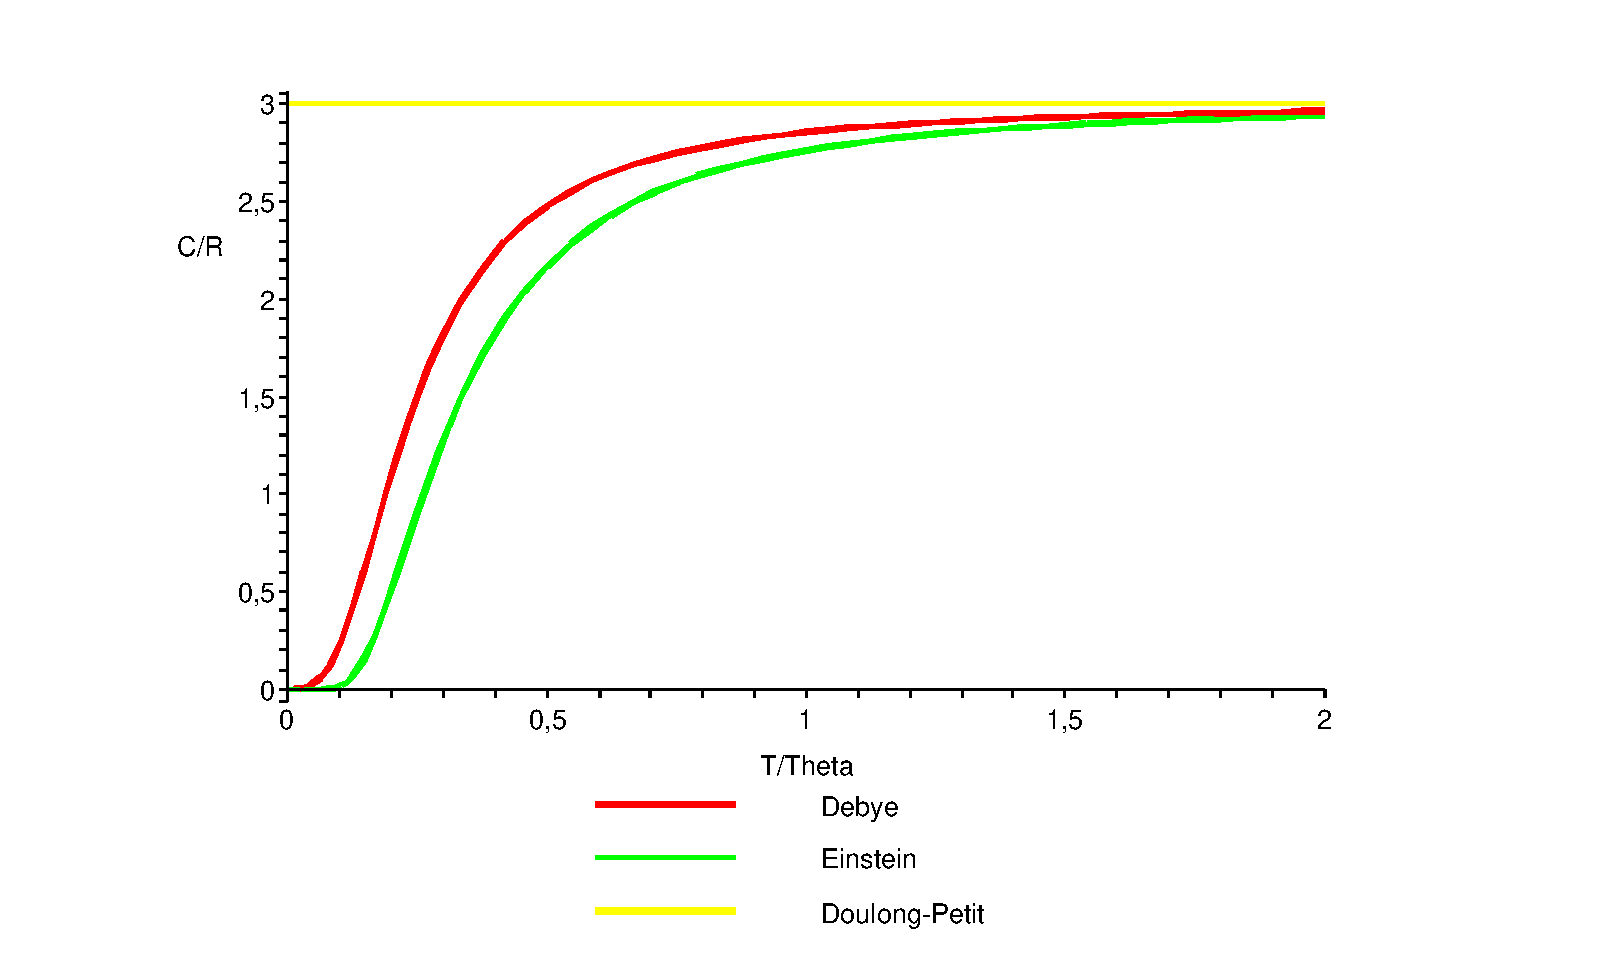
\includegraphics[scale=0.6]{immagini/fisica3/calorispec}
\end{figure}
\index{calore specifico!dei solidi|)}

\chapter{Meccanica statistica}
\minitoc
\section{Boltzmann}
Consideriamo un sistema in equilibrio ad un certa temperatura $T$. Qual è la probabilità di trovare il sistema in equilibrio, isolato dall'ambiente, con energia $E$? Sperimentalmente posso misurare ad intervalli di tempo ravvicinati l'energia interna. Oppure posso prendere diversi sistemi, che comunicano solo con scambi di calore e valutare le loro energie interne. \`E la stessa cosa.

Consideriamo due sistemi $1$ e $2$ a contatto identici in equilibrio termico. La distribuzione di probabilità del primo corpo è uguale a quella del secondo: $P_1=P_2$, perché la probabilità di trovare il primo sistema ad energia $E$ è la stessa di trovare il secondo corpo ad energia $E$. Questa probabilità sarà proporzionale alla temperatura. La probabilità che i due corpi abbiamo energia $E_1$ e $E_2$ rispettivamente è $P(E_1)P(E_2)$. Consideriamo i due sistemi come un unico sistema. Definiamo $P'$ la densità di probabilità di trovare il sistema globale all'energia $E'=E_1+E_2$ e il sistema $1$ all'energia $E_1$ e il sistema $2$ all'energia $E_2$:
\begin{equation}
	P'(E'=E_1+E_2)=P(E_1)P(E_2)
\end{equation}
Ma $P$ e $P'$ sono uguali a meno di un coefficiente in quanto il sistema globale è alla stessa temperatura dei due corpi ed è in equilibrio. Appare chiaro che la funzione cercata è un esponenziale.

Scegliamo $E_1=0$ e $E_2=E$ allora:
\[
	P'(E)=P(0)P(E)=P(E_1)P(E_2)
\]
usando $E=E_1+E_2$:
\[
	P'(E_1+E_2)=P(E_1)P(E_2)=P(0)P(E_1+E_2)
\]
vale per ogni $E_1,E_2$:
\[
	P(E_1+E_2)P(0)=P(E)P(E_2)
\]
se $E_1=E$ e $E_2=\ud E$:
\[
	P(E+\ud E)=\frac{1}{P(0)}P(E)P(\ud E)
\]
\[
	\frac{P(E+\ud E)-P(E)}{\ud E}=\frac{\left(\frac{1}{P(0)}P(E)P(\ud E)\right)-P(E)}{\ud E}=\frac{P(E)}{P(0)}\frac{P(\ud E-P(0)}{\ud E}
\]
\[
	\frac{\ud P(E)}{\ud E}=\frac{P(E)}{P(0)}\frac{\ud P(E=0)}{\ud E}
\]
\[
	\frac{\frac{\ud P(E)}{\ud E}}{P(E)}=\frac{1}{P(0)}\frac{\ud P(E=0)}{\ud E}=-\beta
\]
con $\beta$ indipendente da $E$
\[
	\int_{P(0)}^{P(E)}\frac{\ud P}{P(E)}=\int_0^E-\beta\,\ud E
\]
\begin{equation}
	P(E)=P(0)e^{-\beta E}
\end{equation}
\section{Distribuzione Maxwell--Boltzmann}
Consideriamo un sistema con vari livelli energetici $E_1, E_2, \ldots$ cioè con energia quantizzata. Consideriamo $N$ particelle identiche ma inizialmente distinguibili. Una partizione è una configurazione del sistema, cioè ogni partizione avrà un certo numero di particelle $n_1$ nel livello $E_1$, $n_2$ nel livello $n_2$ \ldots in modo che $\sum n_i=N$. Consideriamo che i livelli energetici siano equalmente accessibili, cioè che tutti gli stati energetici hanno la stessa probabilità di essere occupati. Prendiamo una particolare partizione, quindi fissiamo $n_1, n_2, \ldots$. Vogliamo sapere qual è la probabilità della partizione. Riempiamo il primo livello. Posso scegliere tra $N$ particelle. Ne scelgo una. Per la scelta della successiva ho $N-1$ particelle e così via. Quindi ho:
\begin{equation}
	N(N-1)(N-2)\cdots(N-n_1+1)=\frac{N!}{\left(N-n_1\right)!}
\end{equation}
possibilità\footnote{\[
		N!=N(N-1)(N-2)\cdots(N-n_1+1)\cdot(N-n_1)!
	\]
}\footnote{è una $n_1$-disposizione di $N$ oggetti o disposizione di $N$ oggetti in $n_1$ posti.}. In realtà ci sono $n_1!$ ordini possibili per riempire il livello, ma l'ordine nel nostro caso non conta, quindi dobbiamo dividere per $n_1!$ per far diminuire il numero di scelte\footnote{è una $k$-combinazione di $n$ oggetti o combinazione di $n$ oggetti in $k$ posti}:
\begin{equation}
	\frac{N!}{n_1!(N-n_1)!}
	\label{stat_boltz01}
\end{equation}
conoscendo il calcolo combinatorio quello che si sta cercando è il numero di combinazioni di $N$ oggetti in $n_1$ posti che sono $\binom{N}{n_1}$, che è esattamente la \eqref{stat_boltz01}. Quando passo a riempire il secondo livello con energia $E_2$ partiamo con un numero di particelle ridotto, cioè $N-n_1$. Il numero di combinazioni per riempire $E_2$ è:
\begin{equation}
	\frac{(N-n_1)!}{n_2!(N-n_1-n_2)!}
\end{equation}
Se moltiplichiamo il numero di modi per riempire il primo livello con il numero di modi per riempire il secondo livello troviamo il numero di modi per riempire il primo e il secondo livello:
\begin{equation}
	\frac{N!}{n_1!(N-n_1)!}\frac{(N-n_1)!}{n_2!(N-n_1-n_2)!}=\frac{N!}{n_1!n_2!(N-n_1-n_2)!}
\end{equation}
se continuassimo così per tutti i livelli il numero di modi per riempire tutta la partizione sarebbe\footnote{è una $(n_1,n_2,\ldots)$-multicombinazione di $n$ oggetti distinti}:
\begin{equation}
	P=\frac{N!}{n_1!n_2!n_3!\cdots}
	\label{stat_001}
\end{equation}
\subsubsection{probabilità intrinseca}
Se ora non consideriamo più i livelli energetici equiprobabili, ma gli assegnamo una probabilità intrinseca $g_i$ la probabilità sarà diversa dalla \eqref{stat_001}. Se la probabilità di trovare una particella nel livello $E_i$ è $g_i$ la probabilità di trovare $n_i$ particelle è $g_i^{n_i}$. Quindi la probabilità di una data partizione è:
\begin{equation}
	P=\frac{N!g_1^{n_1}g_2^{n_2}g_3^{n_3}\cdots}{n_1!n_2!n_3!\cdots}
\end{equation}
\subsubsection{indistinguibilità}
Rimoviamo l'ipotesi che le particelle siano distinguibili (in contrasto con l'ipotesi che le particelle siano identiche). Ci sono $N!$ permutazioni di particelle che danno la stessa partizione\footnote{Per esempio posso spostare la particella 1 con la particella 2, o con la tre, \ldots, o con la $N$--esima. Quindi ho $N-1$ possibilità. Poi posso scambiare la secondo particella in $N-2$ modi, così via. Il procedimento non necessariamente doveva iniziare scambiando la particella 1, ma poteva iniziare con $N$ modi diversi.}. Allora la probabilità:
\begin{equation}
	P=\frac{g_1^{n_1}g_2^{n_2}g_3^{n_3}\cdots}{n_1!n_2!n_3!\cdots}=\prod_{i=1}\frac{g_i^{n_i}}{n_i!}
	\label{MB01}
\end{equation}
La \eqref{MB01} esprime la probabilità di una distribuzione Maxwell--Boltzmann\index{distribuzione!Maxwell--Boltzmann}.
\subsection{Equilibrio}
Troviamo lo stato di equilibrio che corrisponde alla partizione più probabile. Dobbiamo gli $n_i$ che massimizzano $P$. Si tratta di un problema di massimi vincolati. I vincoli sono:
\begin{equation}
	\sum_{i} n_i=N
\end{equation}
\begin{equation}
	U=\sum_i n_iE_i
\end{equation}
con $U$ l'energia totale. Esprimiamo il logaritmo di $P$ e massimizziamo questa funzione (il logaritmo è monotono crescente):
\begin{equation}
	\log P= n_1\log g_1+n_2\log g_2+n_3\log g_3+\cdots -\log n_1!-\log n_2! -\log n_3!\cdots
\end{equation}
usando Stirling:
\begin{equation}
	\log x!\sim x\log x-x
\end{equation}
considerando che gli $n_i$ sono grandi.
\begin{equation}
	\begin{split}
		\log P=&n_1\log g_1+n_2\log g_2+n_3\log g_3+\cdots\\
		&-(n_1\log n_1-n1)-(n_2\log n_2-n2)-(n_3\log n_3-n3)-\cdots\\
		=&-n_1\log\frac{n_1}{g_1}-n_2\log\frac{n_2}{g_2}-\cdots+(n_1+n_2+\cdots)\\
		=&N-\sum_i n_i\log\frac{n_i}{g_i}
	\end{split}
\end{equation}
differenziando:
\begin{equation}
	\begin{split}
		\ud\left(\log P\right)&=-\sum_i(\ud n_i)\log\frac{n_i}{g_i}-\sum_i n_i\ud\left(\log\frac{n_i}{g_i}\right)\\
		&=-\sum_i(\ud n_i)\log\frac{n_i}{g_i}-\sum_i n_i\frac{(\ud n_i)}{n_i}\\
		&=-\sum_i(\ud n_i)\log\frac{n_i}{g_i}-\sum_i\ud n_i
	\end{split}
\end{equation}
ma dal primo vincolo:
\begin{equation}
	N=\sum_i n_i\qquad 0=\sum_i\ud n_i
\end{equation}
sostituendo e ponendo uguale a zero:
\begin{equation}
	\ud\left(\log P\right)=\sum\log\frac{n_i}{g_i}\ud n_i=0
\end{equation}
dal secondo vincolo:
\begin{equation}
	U=\sum_i n_iE_i\qquad 0=\sum_i \ud n_iE_i
\end{equation}
Usando due moltiplicatore di Lagrange $\alpha$ e $\beta$ per minimizzare la funzione implicita:
\begin{equation}
	\sum_i\left(\log\frac{n_i}{g_i}\alpha+\beta E_i\right)\ud n_i=0
\end{equation}
quindi:
\[
	\log \frac{n_i}{g_i}+\alpha+\beta E_i=0
\]
invertendo:
\begin{equation}
	n_i=g_ie^{-\alpha-\beta E_i}
\end{equation}
\subsubsection{funzione partizione}
Il numero totale di particelle:
\begin{equation}
	N=\sum_i n_i=\sum_i g_i e^{-\alpha-\beta E_i}=e^{-\alpha}\left(\sum_i g_ie^{-\beta E_i}\right)=e^{-\alpha}Z
\end{equation}
con $Z$ la funzione di partizione:
\begin{equation}
	Z=\sum_i g_i e^{-\beta E_i}
\end{equation}
quindi:
\begin{equation}
	n_i=\frac{N}{Z}g_i e^{-\beta E_i}
	\label{ni_stat}
\end{equation}
che è la legge delle distribuzione di Maxwell--Boltzmann.
\subsubsection{energia media}
L'energia media di un sistema in equilibrio sarà data:
\begin{equation}
	\media{E}=\frac{\sum_i n_iE_i}{N}=\frac{\sum_i \frac{N}{Z}g_i e^{-\beta E_i}E_i}{N}=\frac{1}{Z}\sum_i g_i E_ie^{-\beta E_i}
\end{equation}
o sostituendo $Z$:
\begin{equation}
	\media{E}=\frac{\sum_i g_i E_ie^{-\beta E_i}}{\sum_i g_i e^{-\beta E_i}}
\end{equation}
possiamo anche esprimerla come:
\begin{equation}
	\media{E}=-\frac{\ud}{\ud \beta}(\log Z)
\end{equation}
\subsubsection{energia totale}
L'energia totale:
\begin{equation}
	U=N\media{E}=\frac{N}{Z}\sum_i g_i E_ie^{-\beta E_i}
\end{equation}
o sostituendo $Z$:
\begin{equation}
	U=N\frac{\sum_i g_i E_ie^{-\beta E_i}}{\sum_i g_i e^{-\beta E_i}}
\end{equation}
o anche come:
\begin{equation}
	U=-N\frac{\ud}{\ud \beta}(\log Z)
\end{equation}
\begin{Es}[sistema a due stati equiprobabili]
	consideriamo un sistema con due stati con energia $E_1=\epsilon$ e $E_2=-\epsilon$, equiprobabili, cioè tali che $g_1=g_2=1$. La funzione di partizione:
	\[
		Z=\sum_i g_ie^{-\beta E_i}=e^{-\beta E_1}+e^{-\beta E_2}=e^{-\beta \epsilon}+e^{\beta\epsilon}=2\cosh(\beta\epsilon)
	\]
	all'equilibrio i livelli avranno:
	\[
		\begin{split}
			n_1&=\frac{N}{Z}g_1e^{-\beta E_1}=\frac{N}{2\cosh(\beta\epsilon)}e^{-\beta\epsilon}\\
			n_2&=\frac{N}{Z}g_1e^{-\beta E_2}=\frac{N}{2\cosh(\beta\epsilon)}e^{\beta\epsilon}\\
		\end{split}
	\]
	e l'energia media:
	\[
		\media{E}=\frac{1}{Z}\sum_i g_i E_ie^{-\beta E_i}=\frac{1}{2\cosh(\beta\epsilon)}\left(\epsilon e^{-\beta\epsilon}-\epsilon e^{\beta \epsilon}\right)=-\epsilon\tanh(\beta\epsilon)
	\]
\end{Es}
\section{Temperatura}
Il parametro $\beta$ ha le dimensioni dell'inverso di un energia. La distribuzione dell'energia in un gas perfetto:
\begin{equation}
	\ud n=A\sqrt{E}e^{-\frac{E}{kT}}\ud E
\end{equation}
dalla \eqref{ni_stat} ricaviamo che:
\begin{equation}
	\beta=\frac{1}{kT}
\end{equation}
La definizione di temperatura che ne deriva, cioè come funzione dell'energia interna di un sistema, è valida solo nel caso di particelle in equilibrio termico. Se il nostro sistema non è in equilibrio termico si può dividere il sistema in tanti sottosistemi più piccoli in equilibrio termico.
L'energia media la possiamo scrivere come:
\begin{equation}
	\media{E}=kT^2\frac{\ud}{\ud T}(\log Z)
\end{equation}
e l'energia totale:
\begin{equation}
	U=NkT^2\frac{\ud}{\ud T}(\log Z)
\end{equation}
La distribuzione di Maxwell--Boltzmann diventa:
\begin{equation}
	n_i=\frac{N}{Z}g_ie^{-\frac{E_i}{kT}}
\end{equation}
Se tralasciamo il fattore $g_i$ e fissiamo la temperatura abbiamo un'esponenziale decrescente, quindi avremo molte particelle in stati con energia piccola, minore della media, e poche particelle in stati con energia grande. I livelli energetici più popolati sono quelli con minore energia. All'aumentare della temperatura gli stati con energia maggiore aumentano la loro popolazione e quelli che bassa energia la diminuiscono.

Se consideriamo due livelli con energia $E_i$ e $E_j$ il rapporto delle loro popolazioni è:
\begin{equation}
	\frac{n_j}{n_i}=\frac{\frac{N}{Z}g_je^{-\frac{E_j}{kT}}}{\frac{N}{Z}g_ie^{-\frac{E_i}{kT}}}=\frac{g_j}{g_i}\,e^{-\frac{\Delta E}{kT}}
\end{equation}
\section{Equilibrio termico}
Consideriamo due diversi sottosistemi di particelle che possono scambiare calore tra di loro. Il numero di particelle per ogni sistema rimanga costante. Il primo sistema abbia $N$ particelle, il secondo $N'$. I due sistemi sono isolati dall'esterno, quindi la somma delle loro energie rimane costante:
\begin{align}
	\label{multi_sis_stat01}
	N  & =\sum_i n_i=\const                    \\
	\label{multi_sis_stat02}
	N' & =\sum_j n_j'=\const                   \\
	\label{multi_sis_stat03}
	U  & =\sum_i n_iE_i+\sum_j n_j'E_j'=\const
\end{align}
la probabilità di una particolare partizione di tutto il sistema comprendente i due sottosistemi è:
\begin{equation}
	P=\prod_i\frac{g_i^{n_i}}{n_i!}\cdot\prod_j\frac{g_j'^{n_j'}}{n_j'!}
\end{equation}
per trovare la configurazione all'equilibrio dobbiamo trovare la partizione più probabile. Seguiamo lo stesso procedimento per un sistema singolo. Dalle equazioni \eqref{multi_sis_stat01}, \eqref{multi_sis_stat02}, \eqref{multi_sis_stat03} differenziando:
\begin{align}
	 & \sum_i\ud n_i=0                         \\
	 & \sum_j\ud n_j'=0                        \\
	 & \sum_i E_i\ud n_i+\sum_j E_j'\ud n_j'=0
\end{align}
scriviamo il differenziale del logaritmo (ci permette di passare dai prodotti alle somme) della probabilità e poniamo uguale a zero:
\begin{equation}
	-\ud(\log P)=\sum_i\log\frac{n_i}{g_i}\,\ud n_i+\sum_j\log\frac{n_j'}{g_j'}\,\ud n_j'=0
\end{equation}
usando i moltiplicatori di Lagrange $\alpha$, $\alpha'$ e $\beta$:
\begin{equation}
	\sum_i\left(\log\frac{n_i}{g_i}+\alpha+\beta E_i\right)\,\ud n_i+\sum_j\left(\log\frac{n_j'}{g_j'}+\alpha'+\beta E_j'\right)\,\ud n_j'=0
\end{equation}
quindi:
\begin{equation}
	\log\frac{n_i}{g_i}+\alpha+\beta E_i=0\qquad\log\frac{n_j'}{g_j'}+\alpha'+\beta E_j'=0
\end{equation}
cioè:
\begin{equation}
	n_i=g_ie^{\alpha-\beta E_i}\qquad n_j'=g_j' e^{-\alpha-\beta E_j'}
\end{equation}
e usando le \eqref{multi_sis_stat01} e \eqref{multi_sis_stat02}:
\begin{equation}
	n_i=\frac{N}{Z}g_ie^{-\beta E_i}\qquad n_j'=\frac{N'}{Z'}g_j' e^{-\beta E_j'}
\end{equation}
i due sottosistemi hanno lo stesso $\beta$ poiché la somma delle energie rimane costaten. Sostituendo $\beta$:
\begin{equation}
	n_i=\frac{N}{Z}g_ie^{-\frac{E_i}{kT}}\qquad n_j'=\frac{N'}{Z'}g_j' e^{-\frac{ E_j'}{kT}}
\end{equation}
Concludiamo che due differenti sistemi di particelle in equilibrio statistico devono avere la stessa temperatura, che è il principio zero della termodinamica\index{principio!zero della termodinamica}
All'equilibrio termico ogni sistema raggiunge la stessa configurazione che avrebbe raggiunto all'equilibrio nel caso fosse isolato alla stessa temperatura.


















\chapter{Calore specifico dei gas}
\minitoc
\index{calore specifico!dei gas|(}
Per un gas monoatomico l'energia interna è $E=\frac{3}{2}NkT$, quindi il suo calore specifico molare è $c_v=\frac{1}{n}\frac{\partial}{\partial T} E=\frac{3}{2}R$. Per i gas poliatomici bisogna considerare anche l'energia dovuta alle rotazioni e alle vibrazioni. Il problema è che questi gradi di libertà in più si attivano al variare della temperatura.

Ignoriamo l'enenergia legata agli elettroni. Questi per essere eccitati hanno bisogno di energie dell'ordine di $\SI{1}{\electronvolt}$, cioè di una temperatura di circa $\SI{1E4}{\kelvin}$. A questa temperatura il gas ha subito dei cambiamenti tali che il nostro modello non è più valido. Dopo il grado di libertà traslazionale, che è sempre attivo, si attiva il grado rotazionale. L'energia rotazionale è dell'ordine di $\SI{1E-4}{\electronvolt}$. L'energia vibrazionale invece è maggiore, dell'ordine di $\SIrange{1E-3}{1E-1}{\eV}$ e quindi necessitano una temperatura maggiore per essere attivati. A temperature molto alte tutti i gradi di libertà sono attivati, quindi per una molecola biatomica sono 7 (3 traslazionali, 2 rotazionali e 2 vibrazionali, considerando l'energia potenziale come grado di libertà)\footnote{problema a due corpi: 6 gradi di libertà più uno potenziale}. Quindi l'energia totale in accordo con il principio di equipartizione:
\begin{equation}
	\lim_{T\to\infty}E=\frac{7}{2}NkT
\end{equation}
e il calore specifico:
\begin{equation}
	\lim_{T\to\infty}c_v=\frac{7}{2}R
\end{equation}
\index{calore specifico!dei gas|)}
\section{Calore specifico di gas biatomici}
L'energia totale di ogni molecola è la somma delle energie traslazionali, rotazionali e vibrazionali:
\begin{equation}
	E_\text{tot}=E_\text{tr}+E_\text{rot}+E_\text{vib}
\end{equation}
Stiamo ignorando l'energia legata al moto degli elettroni in quanto per eccittare questo grado di libertà servono temperature talmente alte da alterare la struttura del gas.
\subsubsection{Traslazioni}
Le traslazioni non sono quantizzate, quindi:
\begin{equation}
	U_\text{tr}=\frac{3}{2}nRT
\end{equation}
dal principio di equipartizione.
\subsection{Rotazioni}
Il momento angolare è quantizzato e può avere $2l+1$ possibili orientazioni.
L'energia legata alla rotazione è anch'essa quantizzata:
\begin{equation}
	E_\text{rot}=\frac{\hslash^2l(l+1)}{2I}\qquad l\in\field{N}
\end{equation}
con $I$ il momento di inerzia della molecola relativa all'asse di rotazione per il centro di massa:
\begin{equation}
	I=\mu r_0^2=\frac{m_1m_2}{m_1+m_2}r_0^2
\end{equation}
con $\mu$ la massa ridotta e $m_1$ e $m_2$ le masse degli atomi e $r_0$ la loro distanza. La probabilità intrinseca è uguale per tutti i livelli: $g_i=2l+1$.  La funzione di partizione:
\begin{equation}
	Z_\text{rot}=\sum_i g_i e^{-\frac{E_i}{kT}}=\sum_l(2l+1)e^{-l(l+1)\frac{\Theta_r}{T}}
\end{equation}
con:
\begin{equation}
	\Theta_r=\frac{\hslash^2}{2Ik}
\end{equation}
la temperatura caratteristica rotazionale. Il numero di particelle in un particolare stato rotazionale caratterizzato dal numero $l$:
\begin{equation}
	n_\text{rot}=\frac{N}{Z_\text{rot}}(2l+1)e^{-l(l+1)\frac{\Theta_r}{T}}
\end{equation}
più cresce la temperatura e più molecole si troveranno in stati con $l$ elevato. L'energia totale delle rotazioni:
\begin{equation}
	U_\text{rot}=kNT^2\frac{\ud}{\ud T}\left(\log Z_\text{rot}\right)
\end{equation}
si osserva graficamente che questa funzione passa dal valore di circa $\frac{3}{2}nRT$ al valore $\frac{5}{2}nRT$ in corrispondenza della temperatura caratteristica di rotazione $\Theta_r$.
\subsubsection{approssimazione $T\gg\Theta_r$}
Consideriamo $T\gg\Theta_r$ in modo che l'intervallo tra due livelli rotazionali sia piccolo. Possiamo valutare $Z_\text{rot}$ sostituendo la sommatoria con un integrale. Approssimiamo $2l+1\sim 2l$ e $l(l+1)\sim l^2$:
\begin{equation}
	Z=\int_0^\infty 2le^{-\frac{\Theta_r}{T}l^2}\,\ud l=\frac{T}{\Theta_r}
\end{equation}
e l'energia:
\begin{equation}
	U_\text{rot}=kNT^2\frac{\ud}{\ud T}(\log Z_\text{rot})=kNT^2\frac{\ud}{\ud T}(\log{T}-\log{\Theta_r})=kNT=nRT
\end{equation}
con $n$ numero di moli. Quindi, sempre nel caso $T\gg\Theta_r$:
\begin{equation}
	U=U_\text{tr}+U_\text{rot}=\frac{5}{2}nRT
\end{equation}
e il calore specifico:
\begin{equation}
	c_v=\frac{1}{n}\frac{\partial U}{\partial T}=\frac{5}{2}R
\end{equation}
come vuole la teoria classica.
\subsubsection{approssimazione $T\ll\Theta_r$}
In questo caso l'esponenziale della funzione di partizione decresce molto rapidamente, quindi nella sommatoria dominano solo i primi termini:
\begin{equation}
	Z_\text{rot} = \sum_l(2l+1)e^{-l(l+1)\frac{\Theta_r}{T}}\simeq 1+3e^{-2\frac{\Theta_r}{T}}
\end{equation}
poiché $\frac{\Theta_r}{T}\gg 1$ allora $\log(Z_\text{rot})\simeq 3e^{-2\frac{\Theta_r}{T}}$
e quindi l'energia:
\begin{equation}
	U_\text{rot}=kNT^2\frac{\ud}{\ud T}(\log Z_\text{rot}) = kNT^2 3e^{-2\frac{\Theta_r}{T}} 2\frac{\Theta_r}{T^2} = 6kN e^{-2\frac{\Theta_r}{T}} \Theta_r
\end{equation}
in questo modo se $I\to 0$ ovvero se la distanza tra i due atomi diventa nulla allora il contributo rotazionale sparisce. Questo non succede nel limite classico, cioè quello ad alta energia.
\subsection{Vibrazioni}
L'energia delle vibrazioni è quantizzata come quella di un oscillatore armonico:
\begin{equation}
	E_\text{vib}=(v+\frac{1}{2})\hslash\omega
\end{equation}
e con $g_i=1$. La funzione di partizione:
\begin{equation}
	\begin{split}
		Z_\text{vib}&=\sum_i g_ie^{-\frac{E_i}{kT}}=\sum_v e^{\frac{(-v+\frac{1}{2})\hslash \omega}{kT}}=\sum_v e^{\frac{(-v+\frac{1}{2})\Theta_v}{T}}=e^{-\frac{\Theta_v}{2T}}\left(\sum_v e^{-v\frac{\Theta_v}{T}}\right)\\&=\frac{e^{-\frac{\Theta_c}{2T}}}{1-e^{-\frac{\Theta_v}{T}}}
	\end{split}
\end{equation}
avendo notato che: $|e^{-\frac{\Theta_v}{T}}|<1$ e avendo introdotto la temperatura caratteristica per le vibrazioni: $\Theta_v=\frac{\hslash\omega}{k}$. La temperatura vibrazionale è più alta di quella rotazionale. Il numero di molecole in un certo stato vibrazionale:
\begin{equation}
	n_\text{vib}=\frac{N}{Z_\text{vib}}e^{-(v+\frac{1}{2})\frac{\Theta_v}{T}}
\end{equation}
L'energia legata alle vibrazioni:
\begin{equation}
	\begin{split}
		U_\text{vib}&=kNT^2\frac{\ud}{\ud T}(\log Z_\text{vib})=kNT^2\frac{\ud}{\ud T}\left(\log \frac{e^{-\frac{\Theta_v}{2T}}}{1-e^{-\Theta_v}{T}}\right)\\
		&=kNT^2\frac{\ud}{\ud T}\left(-\frac{\Theta_v}{2T}-\log\left(1-e^{-\frac{\Theta_v}{T}}\right)\right)\\
		&=kNT^2\left(\frac{\Theta_v}{2T^2}+\frac{\frac{\Theta_v}{T^2}}{e^\frac{\Theta_v}{T}-1}\right)=\frac{1}{2}kN\Theta_v+\frac{kN\Theta_v}{e^{\frac{\Theta_v}{T}}-1}
	\end{split}
\end{equation}
il primo addendo $\frac{1}{2}k\Theta_v$ è l'energia vibrazionale di punto zero del gas.
\subsubsection{approssimazione $T\gg\Theta_\text{vib}$}
Il termine al denominatore dell'energia è asintotico per $\frac{\Theta_v}{T}$ piccolo a $\frac{\Theta_v}{T}$, quindi l'energia per alte temperature diventa:
\begin{equation}
	U_\text{vib}=\frac{1}{2}kN\Theta_v+kNT=kNT\left(1+\frac{\Theta_v}{2T}\right)\simeq KNT=nRT
\end{equation}
e l'energia totale:
\begin{equation}
	U=U_\text{tr}+U_\text{rot}+U_\text{vib}=\frac{3}{2}nRT+nRT+nRT=\frac{7}{2}nRT
\end{equation}
e il calore specifico:
\begin{equation}
	c_V=\frac{1}{n}\frac{\partial}{\partial T}U=\frac{7}{2}R
\end{equation}
\subsubsection{calore specifico vibrazionale}
\begin{equation}
	\begin{split}
		c_V^{\text{vib}}&=\frac{1}{n}\frac{\ud}{\ud T}U_\text{vib}=\frac{1}{n}\frac{\ud}{\ud T}\left(\frac{1}{2}kN\Theta_v+\frac{kN\Theta_v}{e^{\frac{\Theta_v}{T}}-1}\right)\\
		&=R\left(\frac{\Theta_V}{T}\right)^2\frac{e^{\frac{\Theta_V}{T}}}{\left(e^{\frac{\Theta_V}{T}}-1\right)^2}
	\end{split}
\end{equation}
praticamente identico (a parte il fattore $3$) al calore specifico dei solidi secondo Einstein.









\chapter{Scattering}
\minitoc
\section{Particelle \texorpdfstring{$\alpha$}{alfa}}
Osservando il decadimento di uranio osservò due tipi di radiazioni $\alpha$ e $\beta$. Con un esperimento simile a quello di Thomson per il rapporto carica--massa dell'elettrone misurò il rapporto carica--massa delle particelle $\alpha$ arrivando ad un valore che erà metà di quello del protone. Analizzando lo spettro di emissione delle particelle $\alpha$ concluse che le particelle $\alpha$ altro non erano che $\mathrm{He}^{2+}$. Infatti\footnote{Dai dati sperimentali nella sezione risulta
	\[
		0.503448683\pm 3.47\times 10^{-7}
	\]
}
:
\[
	\frac{q_{\mathrm{He^{2+}}}}{m_{\mathrm{He}^{2+}}}=\frac{2q_{\mathrm{p}^+}}{4m_{\mathrm{p}^+}}=\frac{1}{2}\frac{q_{\mathrm{p}^+}}{m_{\mathrm{p}^+}}
\]
Thomson usò queste particelle per i suoi esperimenti sfruttando la loro grande massa ed energia.
\section{Scattering di Thomson}
\subsubsection{modello di Thomson}
Il modello di Thomson descrive il nucleo come una densità di carica positiva che contiene gran parte della massa atomica in cui sono immersi gli elettroni, in modo che all'esterno l'atomo risulti neutro. Questo modello viene escluso dagli esperimenti di scattering di Ruttherford.  Gli esperimenti di scattering avvenivano su vari metalli: un fascio collimato di particelle $\alpha$ colpiva nel vuoto una sottile lamina metallica. Le particelle che passavano colpivano uno schermo che si illuminava quando veniva colpito. In questo modo era possibile misurare gli angoli di scattering. Gran parte delle particelle erano deviate di angoli molto piccoli, dell'ordine di $\SI{1}{\degree}$. Tuttavia in modo inastpettato alcune particelle erano deviate di $\SI{90}{\degree}$ o più. Se assumiamo il modello di Thomson per avere una deflessione della traiettoria la particella $\alpha$ deve entrare nell'atomo, cioè nella densità di carica positiva, perché all'esterno la particella $\alpha$ vede l'atomo neutro.

Consideriamo la collisione di una particella $\alpha$ con un elettrone. Essendo la massa della particella $\alpha$ circa $7294$ volte la massa dell'elettrone possiamo dire $m_\alpha\gg m_{\mathrm{e}}$. Dalla teoria sugli urti, imponendo la conservazione della quantità di moto e dell'energia cinetica, considerando il caso monodimensionale e considerando il caso limite\footnote{vedi \ref{casilimiteurti} a pag.\@\pageref{casilimiteurti}} $m_\alpha\gg m_{\mathrm{e}}$ con l'elettrone inizialmente fermo si ha che dopo l'urto la particella $\alpha$ prosegue con la velocità che aveva prima dell'urto, mentre l'elettrone acquista una velocità pari a due volte quella della particella $\alpha$. Se vogliamo una deviazione della traiettoria della particella $\alpha$ dobbiamo far si che l'urto avvenga di striscio. Ipotizzando il caso di deviazione massima, cioè quando $\Delta \ve p_\alpha$ è ortogonale a $\ve p_\alpha$ abbiamo che $\frac{\Delta p_\alpha}{p_\alpha}=\tan\theta\sim\theta$. Facendo i conti a caso, dicendo che $\Delta p_\alpha$ è uguale a $-\Delta p_\mathrm{e}=2m_\mathrm{e}v_\alpha\simeq 2m_\alpha v_\alpha/7294$ si ottiene che $\theta\sim \SI{0.01}{\degree}$.

Consideriamo l'effetto della carica positiva. Una sfera di raggio $R$ uniformente carica con carica totale $Q$ produce una forza su una particella $\alpha$ a distanza $r$ dal centro:
\begin{equation}
	F=\left\{\begin{array}{ll}
		\dfrac{Qq_\alpha}{4\pi\varepsilon_0}\dfrac{r}{R^2} & r\leq R \\
		\dfrac{Qq_\alpha}{4\pi\varepsilon_0}\dfrac{1}{r^2} & r\geq R \\
	\end{array}\right.
\end{equation}
il massimo della forza si ha per $r=R$. Assumiamo che la forza agisca solo quando la particella $\alpha$ è all'interno della distribuzione di carica, cioè per un tempo $\Delta t\sim\frac{2R}{v}$. Supponiamo che la forza sia sempre quella massima. La variazione di quantità di moto:
\[
	\Delta p\sim F\Delta t=\frac{q_\alpha Q}{4\pi\varepsilon_0}\frac{1}{R^2}\frac{2R}{v}
\]
ipotizzando il caso di deviazione massima, cioè quando $\Delta\ve p\perp\ve p$ si ha:
\[
	\tan\theta=\frac{\Delta p}{p}\sim\frac{q_\alpha Q}{4\pi\varepsilon_0}\frac{1}{R^2}\frac{2R}{m_\alpha v^2}=\frac{q_\alpha Q}{4\pi\varepsilon_0}\frac{1}{R\left(\frac{1}{2}m_\alpha v^2\right)}
\]
se assumiamo $q_\alpha=2e$ con un'energia di $\SI{5}{\mega\electronvolt}$, incidente su una lastra di oro con $Q=79e$ e $R=\SI{1}{\angstrom}$ abbiamo:
\[
	\theta\sim\tan\theta=\SI{0.026}{\degree}
\]

Secondo questo calcolo pedestre la maggior parte delle particelle dovrebbe essere scatterata con un angolo di $\SI{1}{\degree}$. Si può dimostrare che la frazione di particelle scatterate con un angolo maggiore di $\theta$ è $e^{-(\theta/\media{\theta})^2}$. Se assumiamo $\media{\theta}=\SI{1}{\degree}$ allora la frazione scatteerata con angolo maggiore di $\SI{90}{\degree}$ è $e^{-(90/1)^2}\simeq 10^{-3500}$. La frazione osservata da Ruttherford era di $\frac{1}{8000}$, in disaccordo col modello di Thomson. L'atomo di Thomson non è in grado di deflettere abbastanza le particelle $\alpha$.

Se ora proviamo a calcolare quale deve essere il raggio dell'atomo (prima avevamo assunto $\SI{1}{\angstrom}$) per avere uno scattering di $\SI{1}{\degree}$:
\[
	R=\frac{q_\alpha Q}{4\pi\varepsilon_0}\frac{1}{\frac{1}{2}m_\alpha v^2}=\SI{4.6E-4}{\angstrom}
\]
Ruttherford concluse che per avere angoli di scattering come quelli osservati la carica positiva doveva avere un volume molto piccolo rispetto al volume dell'atomo.
\section{Scattering di Ruttherford}
Assumiamo che la carica del nucleo scatteratore sia concentrata nel nucleo, molto piccolo, posto nell'origine delle coordinate. Definiamo il parametro di impatto $b$ la distanza tra l'asintoto della traiettoria della particella $\alpha$ per $t\to-\infty$ e il nucleo scatteratore. Vogliamo sapere l'angolo $\theta$ tra la direzione dell'asintoto per $t\to-\infty$ e la direzione dell'asintoto per $t\to\infty$.
\subsubsection{Distanza di minimo avvicinamento}
L'energia meccanica è una costante del moto:
\begin{equation}
	E=K+V=\const
\end{equation}
all'infinito l'energia potenziale è nulla e l'energia è tutta energia cinetica; al contrario alla distanza di minimo avvicinamento $\Delta$ l'energia è tutta potenziale:
\begin{multline}
	E=K(\infty)+V(\infty)=K(\infty)=\frac{1}{2}mv_0^2=\\=E=K(\Delta)+V(\Delta)=V(\Delta)=\frac{Zze^2}{\giorgi\Delta}
\end{multline}
con $Z$ il numero di protoni nel nucleo, ognuno di carica $e$, $z$ il numero di protoni della particella $\alpha$ (2). Allora:
\begin{equation}
	\Delta=\frac{1}{\giorgi}\frac{zZe^2}{E}
\end{equation}
\subsubsection{Orbita}
Calcoliamo l'orbita della particella $\alpha$ nel campo di forze centrale. Lavoriamo in coordinate polari. Il moto è piano e il momento angolare $\ve L$ è costante del moto:
\begin{equation}
	\begin{aligned}
		L= & \left\|\ve r\times m\ve v\right\|=\left\|mr \ver u_r\times(\dot r\ver u_r+r\dot\varphi\ver u_\varphi)\right\|=mr^2\dot\varphi \\
		=  & L(t=-\infty)=mvb
	\end{aligned}
\end{equation}
quindi la variabile angolare:
\begin{equation}
	\dot\varphi=\frac{L}{mr^2}
\end{equation}
essendo $\dot\varphi\gtrless0$ allora $\varphi$ sarà una funzione monotona.
L'accelerazione centripeta:
\begin{equation}
	a_r=\ddot r-r\dot\varphi^2
\end{equation}
e la forza centripeta è uguale alla forza coulombiana:
\begin{equation}
	ma_r=m\left(\ddot r-r\dot\varphi^2\right)=\frac{1}{\giorgi}\frac{zZe^2}{r^2}
	\label{scatter_cou_acc}
\end{equation}
cambiamo variabile e ricalcoliamo le derivate per poi sostituirle nella \eqref{scatter_cou_acc} considerando $r=r(u)$, $u=u(\varphi)$, $\varphi=\varphi(t)$:
\begin{subequations}
	\begin{equation}
		u=\frac{1}{r}
	\end{equation}
	\begin{gather}
		\frac{\ud\varphi}{\ud t}=\frac{L}{mr^2}=\frac{L}{m}u^2\\
		\frac{\ud r}{\ud t}=\frac{\ud r}{\ud u}\frac{\ud u}{\ud \varphi}\frac{\ud \varphi}{\ud t}=-\frac{1}{u^2}\frac{\ud u}{\ud\varphi}\frac{L}{m}u^2=-\frac{L}{m}\frac{\ud u}{\ud\varphi}\\
		\frac{\ud^2 r}{\ud t^2}=\frac{\ud}{\ud\varphi}\left(\frac{\ud r}{\ud t}\right)\frac{\ud\varphi}{\ud t}=-\frac{L}{m}\frac{\ud^2 u}{\ud\varphi^2}\frac{L}{m}u^2\\
	\end{gather}
\end{subequations}
sostituendo nella \eqref{scatter_cou_acc}:
\begin{equation}
	m\left(-\frac{L^2}{m^2}u^2\frac{\ud^2 u}{\ud\varphi^2}-\frac{1}{u}\frac{L^2}{m^2}u^4\right)=\frac{zZe^2}{\giorgi}u^2
\end{equation}
dividento per $-\frac{L^2}{m}u^2$:
\begin{equation}
	u''+u=-\frac{zZe^2}{\giorgi}\frac{m}{L^2}
\end{equation}
Ricordando:
\begin{gather*}
	\Delta=\frac{1}{\giorgi}\frac{zZe^2}{E}=\frac{1}{\giorgi}\frac{zZe^2}{\frac{1}{2}mv_0^2}\\
	L^2=m^2v_0^2b^2
\end{gather*}
\begin{equation}
	u''+u=-\frac{zZe^2}{\giorgi}\frac{m}{L^2}=-\frac{zZe^2}{\giorgi}\frac{m}{m^2v_0^2b^2}=-\frac{zZe^2}{\giorgi}\frac{m}{m^2v_0^2b^2}=-\frac{\Delta}{2b^2}
\end{equation}
Per risolvere l'equazione differenziale. Omogenea associata:
\[
	\lambda^2-1=0\qquad \lambda=\pm i\qquad u(\varphi)=A\sin\varphi+B\cos\varphi
\]
quindi l'equazione differenziale ha soluzione generale:
\begin{equation}
	u(\varphi)=A\sin\varphi+B\cos\varphi-\frac{\Delta}{2b^2}
\end{equation}
imponendo le condizioni iniziali:
\begin{equation}
	\{r\to-\infty\Leftrightarrow u\to 0\Rightarrow\varphi\to 0\}\Leftrightarrow u(0)=0
\end{equation}
\begin{equation}
	u(0)=B-\frac{\Delta}{2b^2}=0\Rightarrow B=\frac{\Delta}{2b^2}
\end{equation}
e
\begin{equation}
	\left\{v(\varphi=0)=\dot r(t=-\infty)=-\left.\frac{L}{m}\frac{\ud u}{\ud \varphi}\right|_{\varphi=0}=(-v_0\ver u_r)_r=-v_0=-\frac{L}{mb}\right\}\Leftrightarrow
	\left.\frac{\ud u}{\ud \varphi}\right|_{\varphi=0}=\frac{1}{b}
\end{equation}
\begin{equation}
	\left.\frac{\ud u}{\ud \varphi}\right|_{\varphi=0}=A=\frac{1}{b}
\end{equation}
In definitiva l'equazione del moto:
\begin{equation}
	\frac{1}{r}=\frac{1}{b}\sin\varphi+\frac{\Delta}{2b^2}\left(\cos\varphi-1\right)
\end{equation}
che è l'equazione di un iperbole.
%\begin{figure}[htbp]
%  \centering
%  \input{immagini/fisica3/traiettoria_ruth}
%  \caption{Traiettoria.}
%\end{figure}
\subsubsection{angolo di scattering}
Calcoliamo gli asintoti dell'orbita per $r\to\pm\infty$ in funzione dell'angolo di scattering $\theta=\pi-\varphi$:
\[
	0=\frac{1}{b}\sin\theta+\frac{\Delta}{2b^2}\left(-\cos\theta-1\right)
\]
una soluzione è $\theta = \pi$ che corrisponde a $t\to -\infty$. L'altra si trova ricordando che $\sin\theta=2\sin(\theta/2)\cos(\theta/2)$ e che $1+\cos\theta=2\cos^2(\theta/2)$:
\begin{gather*}
	0=\frac{1}{b}\left(2\sin\left(\frac{\theta}{2}\right)\cos\left(\frac{\theta}{2}\right)-\frac{\Delta}{2b}2\cos^2\left(\frac{\theta}{2}\right)\right)\\
	\sin\left(\frac{\theta}{2}\right)-\frac{\Delta}{2b}\cos\left(\frac{\theta}{2}\right)=0
\end{gather*}
da cui si ricava la legge dello scattering coulombiano:
\begin{equation}
	b=\frac{\Delta}{2}\cot\left(\frac{\theta}{2}\right)
\end{equation}
che lega il parametro d'impatto (la condizione iniziale) all'angolo di scattering (la condizione finale).
\section{Analisi scattering}
Consideriamo lastre molto sottili, quindi escludiamo la possibilità che le particelle $\alpha$ subiscano più scattering. Il numero $n$ di nuclei scatteratori si può ricavare dalla densità $\rho$ del bersaglio, lo spessore $\delta$ e la sua area $A$, infatti:
\[
	\rho=\frac{M}{V}=\frac{n\mathcal{M}}{N_A\delta A}
\]
con $\mathcal{M}$ la massa molare. Invertendo:
\begin{equation}
	n=\frac{\rho N_A}{\mathcal{M}}\delta A
\end{equation}
L'intensità del fascio $I_0$ è il numero $N_\alpha$ di particelle $\alpha$ per unità di tempo e unità di area, quindi nell'unità di tempo
\begin{equation}
	N_\alpha=I_0A
\end{equation}

Se voglio conoscere le particelle con angolo di scattering $\theta>\theta_0$ allora essendo la cotangente una funzione decrescente saranno quelle particelle con un parametro $b<b_0=\frac{\Delta}{2}\cot\left(\frac{\theta_0}{2}\right)$. Il numero di queste particelle per unità di tempo è il numero di particelle contenute nella circonferenza di raggio $b_0$ moltiplicato per l'intensità: $\pi b_0^2I_0$. La quantità $\pi b_0^2$ è la sezione d'urto per angoli maggiori di $\theta_0$. La sezione d'urto è definita come il numero di particelle scatterate con una certa proprietà diviso l'intensità del fascio. Considerando che ci sono $n$ scatteratori allora il numero di particelle scatterate con angolo maggiore di $\theta_0$ è $\pi b_0^2I_0\frac{\rho N_A}{\mathcal{M}}\delta A$. Se vogliamo la frazione di particelle dobbiamo dividere per il numero di particelle $\alpha$ totali $I_0A$ e quindi la frazione di particelle scatterate con angolo maggiore di $\theta_0$ risulta:
\begin{equation}
	\chi=\pi b_0^2\frac{\rho N_A}{\mathcal{M}}\delta
\end{equation}
\subsection{Sezione d'urto differenziale}
Vogliamo calcolare quante particelle vengono scatterate con angolo compreso tra $\theta$ e $\theta+\ud\theta$. Esse sono quelle particelle scatterate sull'angolo solido $\ud\Omega$:
\begin{equation}
	\ud S=2\pi R\sin\theta (R\ud\theta)\qquad\ud\Omega=\frac{\ud S}{R^2}=2\pi\sin\theta\ud\theta
\end{equation}
Il numero di particelle nell'unità di tempo $\ud N$ con parametro compreso tra $b$ e $b+\ud b$ sono quelle che verranno scatterate con angolo tra $\theta$ e $\theta+\ud\theta$. Esse sono:
\begin{equation}
	\ud N=I_0 n2\pi b\ud b
\end{equation}
con $n$ il numero di scatteratori. Definiamo la sezione d'urto differenziale per un singolo nucleo scatteratore:
\begin{equation}
	\ud\sigma=\frac{\ud N}{nI_0}=2\pi b\ud b
\end{equation}
che è proprio l'area da dove provengono le particelle che ci interessano, cioè quelle scatterate sull'angolo solido $\ud\Omega$. Calcoliamo $\ud b$ essendo $b=\frac{\Delta}{2}\cot\theta/2$:
\begin{equation}
	\ud b=\frac{\Delta}{2}\frac{-\sin^2\left(\frac{\theta}{2}\right)-\cos^2\left(\frac{\theta}{2}\right)}{\sin^2\left(\frac{\theta}{2}\right)}\frac{1}{2}\ud\theta=-\frac{\Delta}{4}\frac{1}{\sin^2\left(\frac{\theta}{2}\right)}\,\ud \theta
\end{equation}
sostituendo:
\begin{equation}
	\begin{split}
		\ud\sigma&=\frac{\ud N}{nI_0}=2\pi b\ud b=2\frac{\Delta}{2}\cot\left(\frac{\theta}{2}\right)\frac{\Delta}{4}\frac{1}{\sin^2\left(\frac{\theta}{2}\right)}\,\ud \theta=\frac{\pi\Delta^2}{4}\frac{\cos\left(\frac{\theta}{2}\right)}{\sin^3\left(\frac{\theta}{2}\right)}\\
		&=\frac{\pi\Delta^2}{4}\frac{\cos\left(\frac{\theta}{2}\right)\sin\left(\frac{\theta}{2}\right)}{\sin^4\left(\frac{\theta}{2}\right)}=\frac{\pi\Delta^2}{8}\frac{\sin\theta}{\sin^4\left(\frac{\theta}{2}\right)}\,\ud\theta=\frac{\,\Delta^2}{16}\frac{1}{\sin^4\left(\frac{\theta}{2}\right)}\,\ud\Omega
	\end{split}
\end{equation}
\begin{figure}[htbp]
	\centering
	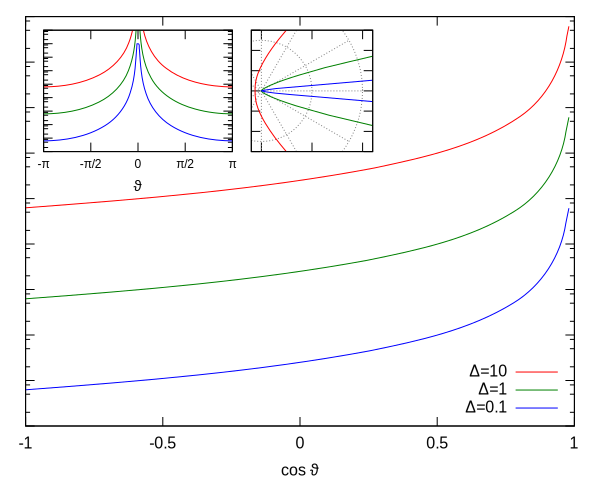
\includegraphics[scale=0.6]{immagini/fisica3/sezione_coulomb}
	% sezione_coulomb.pdf: 480x384 pixel, 72dpi, 16.93x13.55 cm, bb=0 0 480 384
	\caption{Sezione d'urto differenziale per lo scattering di Coulomb. Gli assi verticali sono logaritmici, il secondo grafico piccolo è un grafico polare. Le curve con $\Delta$ piccolo corripondono a fasci con particelle più energetiche.}
	\label{fig:sezione_coulomb}
\end{figure}
a volte la sezione d'urto differenziale viene scritta come:
\begin{equation}
	\frac{\ud\sigma}{\ud\Omega} = \frac{1}{4}z^2 Z^2\left(\frac{\hslash c}{E}\right)^2\alpha^2\frac{1}{(1-\cos\theta)^2}
\end{equation}
per confrontarlo con altri scatterig. Si noti che non è un processo quantistico infatti gli $\hslash$ si semplificano.
\subsection{Raggio nucleare}
Per stimare il raggio nucleare: sia $A$ il numero di nucleoni $r_\text{nucleone}\simeq \SI{1.4E-15}{\meter}$ il raggio di un nucleone, allora il volume di tutto il nucleo:
\[
	A\frac{4}{3}\pi r^3_\text{nucleone}\!\!=\frac{4}{3}\pi r^3_\text{nucleo}
\]
invertendo:
\begin{equation}
	r_\text{nucleo}\simeq r_\text{nucleone}A^{\frac{1}{3}}
\end{equation}










\chapter{Atomo}
\minitoc
\section{Formula di Rydeberg--Ritz}
Un gas eccitato da una scarica elettrica emette una radiazione discreta, a bande, ognuna caratterizzata da una lunghezza d'onda. Per lo spettro di emissione dell'idrogeno Balmer scoprì che seguivano un'andamento:
\begin{equation}
	\frac{1}{\lambda}=R\left(\frac{1}{m^2}-\frac{1}{n^2}\right)\qquad n,m\in\field{N}\qquad n>m
	\label{Ritz}
\end{equation}
$R$ è la costante di Rydberg che varia in modo regolare da elemento a elemento e tende a $R_\infty$ per elementi pesanti.
\section{Modello di Bohr}
Come Ruttherford Bohr assunse che gli elettroni di un atomo si muovessero su orbite intorno al nucleo positivo. Il modello non è stabile, perché gli elettroni in moto accelerato irradiano e quindi perdono energia. In questo modo l'orbita dell'elettrone dovrebbe diventare sempre più piccola. Poiché la frequenza emessa da un elettrone in orbita circolare intorno al nucleo è la frequenza del moto si avrebbe uno spettro continuo.

Bohr postulò che un elettrone si può muovere su certe orbite senza irradiare. Chiamò queste orbite stati stazionari. In questo modo le orbite sono quantizzate. Ogni modello quantizzato deve rispettare il principio di corrisponenza cioè quando consideriamo il limite di grandi orbite o grandi energie, molto più grandi del quanto, la teoria quantistica deve contemplare il risultato classico.

Durante il passaggio da uno stato stazionario ad energia $E_i$ ad un altro con energia $E_2$ l'elettrone emette onde elettromagnetiche con frequenza tale che:
\begin{equation}
	-\Delta E = E_i-E_f=h\nu
\end{equation}
questo tiene conto della conservazione dell'energia. Infatti se inizialmente l'elettrone aveva energia $E_i$ alla fine ha energia $E_f$ ma ha emesso un fotone con energia $h\nu$:
\begin{equation}
	E_i=E_f+h\nu
\end{equation}

Dalla teoria di Bohr e dal principio di corrispondenza segue che il momento angolare $l$ deve essere quantizzato:
\begin{equation}
	l=n\hslash\qquad n\in\field{N}
\end{equation}

Consideriamo un atomo con numero atomico $Z$ e un elettrone. La velocità in funzione del raggio:
\begin{equation}
	\frac{m_{\mathrm{e}}v^2}{r}=\frac{1}{4\pi\varepsilon_0}\frac{Ze^2}{r^2}\qquad v^2=\frac{1}{\giorgi}\frac{Ze^2}{m_{\mathrm{e}}r}
	\label{bohr02}
\end{equation}
L'energia dell'orbita dell'elettrone è:
\begin{equation}
	E=\frac{1}{2}m_{\mathrm{e}}v^2-\frac{Ze^2}{\giorgi}\frac{1}{r}=\frac{1}{2}m_{\mathrm{e}}\frac{1}{\giorgi}\frac{Ze^2}{m_{\mathrm{e}}r}-\frac{Ze^2}{\giorgi}\frac{1}{r}=-\frac{1}{2}\frac{1}{\giorgi}\frac{Ze^2}{r}
	\label{BohrEn}
\end{equation}
Il momento angolare è quantizzato:
\begin{equation}
	l=m_{\mathrm{e}}vr=n\hslash\qquad v=\frac{n\hslash}{m_{\mathrm{e}}r}
	\label{bohrv01}
\end{equation}
confrontandola con la \eqref{bohr02}:
\begin{equation}
	v^2=\frac{n^2\hslash^2}{m_{\mathrm{e}}^2r^2}=\frac{1}{\giorgi}\frac{Ze^2}{m_{\mathrm{e}}r}
\end{equation}
trovando $r$:
\begin{equation}
	r=n^2\frac{\hslash^2\giorgi}{m_{\mathrm{e}}Ze^2}=n^2\frac{a_0}{Z}
	\label{Bohr04}
\end{equation}
con $a_0=\frac{\hslash^2\giorgi}{m_\mathrm{e}e^2}\simeq \SI{0.529}{\angstrom}$ il primo raggio di Bohr\index{raggio!di Bohr}. Al variare di $n\in\field{N}$ la \eqref{Bohr04} rappresenta il raggio di tutte le orbite stabili.

Per la velocità sostituiamo nell'espressione \eqref{bohrv01} ricavata dalla quantizzazione del momento angolare il valore del raggio per le orbite stabili \eqref{Bohr04}:
\begin{equation}
	v=\frac{n\hslash}{m_{\mathrm{e}}r}=\frac{n\hslash Z}{m_{\mathrm{e}}n^2a_0}=\frac{\hslash Z}{nm_\mathrm{e}a_0}=\frac{\hslash Z m_\mathrm{e} e^2}{n m_\mathrm{e}\giorgi\hslash^2}=\frac{Ze^2}{\giorgi\hslash}\frac{1}{n}=\frac{Z}{n}\alpha c
\end{equation}
La velocità dell'elettrone nella prima orbita dell'atomo di idrogeno ($Z=1$):
\begin{equation}
	v_1=v(n=1)=\frac{e^2}{\giorgi\hslash}
\end{equation}
definiamo la costante di struttura fine:
\begin{equation}
	\alpha=\frac{v_1}{c}=\frac{e^2}{\giorgi\hslash c}=\frac{e^2}{2\varepsilon_0hc}\simeq\frac{1}{137}
\end{equation}


Sostituendo la \eqref{Bohr04} nell'espressione dell'energia \eqref{BohrEn} troviamo l'energia quantizzata:
\begin{equation}
	\begin{split}
		E&=-\frac{1}{2}\frac{1}{\giorgi}\frac{Ze^2}{r}=-\frac{1}{2}\frac{1}{\giorgi}\frac{Ze^2}{n^2\frac{a_0}{Z}}=-\frac{1}{2}\frac{1}{\giorgi}\frac{e^2}{a_0}Z^2\frac{1}{n^2}\\
		&=-\frac{1}{2}\frac{1}{(\giorgi)^2}\frac{m_{\mathrm{e}}e^4}{\hslash^2}\frac{Z^2}{n^2}\\
		&=-\frac{Z^2e^4m_\mathrm{e}}{8\varepsilon_0^2h^2}\frac{1}{n^2}\\
		&=-\frac{Z^2R_\infty hc}{n^2}=-Z^2\frac{E_0}{n^2}
	\end{split}
\end{equation}
con
\begin{equation}
	R_\infty=\frac{m_e e^4}{8\varepsilon_0^2h^3 c}=\frac{\alpha^2m_\mathrm{e}c}{2h}\simeq \SI{1.0974E7}{\per\metre}
\end{equation}
\begin{equation}
	E_0=\frac{1}{(\giorgi)^2}\frac{m_{\mathrm{e}}e^4}{2\hslash^2}=\frac{\alpha^2}{2}m_\mathrm{e}c^2=R_\infty hc\simeq \SI{13.6}{\electronvolt}
\end{equation}
l'energia della prima orbita che corrisponde quindi all'energia che devo fornire ad un atomo per strappare l'elettrone sul livello più basso, che è l'energia di ionizzazione. Il salto energetico di un elettrone che passa da $n=n_1$ a $n=n_2$:
\begin{equation}
	\Delta E=E_2-E_1=-Z^2R_\infty hc\left(\frac{1}{n_2}-\frac{1}{n_1}\right)
\end{equation}
La frequenza del fotone emesso quando un elettrone passa da $E_1$ a $E_2$:
\begin{equation}
	\nu=\frac{-\Delta E}{h}={Z^2R_\infty c}\left(\frac{1}{n_2^2}-\frac{1}{n_1^2}\right)
\end{equation}
Possiamo vedere se è coerente con la formula di Ryedberg--Ritz \eqref{Ritz} calcolando:
\begin{equation}
	\frac{1}{\lambda}=\frac{\nu}{c}=Z^2R_\infty\left(\frac{1}{n_2^2}-\frac{1}{n_1^2}\right)
\end{equation}
naturalmente la forumula di Ryedberg--Ritz prende in considerazione solo l'idrogeno, quindi $Z=1$.
\subsection{Correzione massa}
Abbiamo assunto che il nucleo sia fermo, oppure che abbia massa infinita: abbiamo considerato il problema ad un corpo. Poiché le forze in gioco sono classiche per considerare il problema a due corpi basta sostituire alla massa dell'elettrone la massa ridotta $\mu$ del sistema elettrone--nucleo:
\begin{equation}
	\mu=\frac{m_\mathrm{e}Zm_\mathrm{p}}{m_\mathrm{e}+Zm_\mathrm{p}}
\end{equation}
con $m_\mathrm{p}$ la massa del protone. Definiamo:
\begin{equation}
	R=\frac{\mu e^2}{8\varepsilon_0^2h^3 c}=R_\infty\frac{\mu}{m_\mathrm{e}}\xrightarrow{Z\to\infty} R_\infty
\end{equation}
\begin{Es}[Riga $\mathrm{H}_\alpha$]
	La riga $\mathrm{H}_\alpha$ è quella corrispondente alla transizione $n=3\to2$ nell'idrogeno. Calcoliamo il numero d'onda
	\begin{multline*}
		\frac{1}{\lambda}=R\left(\frac{1}{n_2}-\frac{1}{n_1}\right)=R_\infty\frac{\mu}{m_\mathrm{e}}\left(\frac{1}{2^2}-\frac{1}{3^2}\right)=\frac{5}{36}R_\infty\frac{Zm_\mathrm{p}}{Z m_\mathrm{p}+m_\mathrm{e}}\\=\frac{5}{36}R_\infty\frac{1}{1+\frac{m_\mathrm{e}}{m_\mathrm{p}}}\simeq \SI{1.523E6}{\per\meter}
	\end{multline*}
	avendo usato $n_1=3$, $n_2=2$ e $Z=1$. La lunghezza d'onda:
	\[
		\lambda\simeq \SI{6.565E-7}{\meter}=\SI{656.5}{\nano\meter}
	\]
	Se avessimo usato $R_\infty$ al posto di $R$ sarebbe risultato: $\lambda\simeq \SI{6.561E-7}{\meter}$. Infatti la correzione per l'idrogeno della massa ridotta:
	\[
		\mu_\mathrm{H}=\frac{m_\mathrm{e}m_\mathrm{p}}{m_\mathrm{e}-m_\mathrm{p}}=\frac{1}{1+\frac{m_\mathrm{e}}{m_\mathrm{p}}}m_\mathrm{e}\simeq 1.0005 \times m_\mathrm{e}
	\]
\end{Es}
\subsection{Correzione relativistica}
Un'estensione del modello di Bohr potrebbe essere quella di usare orbite ellittiche al posto che circolari. In questo caso l'energia dell'orbita dipenderebbe solamente dall'asse maggiore dell'ellisse e non dall'ecentricità.

Sommerfeld\index{Sommerfeld} anallizzò gli effetti della relatività ristretta sul modello di Bohr. Un orbita molto eccentrica avrà una correzione relativistica più grande essedo il fattore $\beta$ grande. Per orbite circolari:
\begin{equation}
	v=\frac{Z}{n}\alpha c
\end{equation}
quindi:
\begin{equation}
	\beta=\frac{v}{c}=\frac{Z}{n}\alpha
	\label{betabohr}
\end{equation}
Se si analizzano molto in dettaglio delle linee spettrali dell'idrogeno si nota che esse consistono in diverse righe molto vicine. Nella teoria di Sommerfeld è spiegato dicendo che per ogni orbita circolare di raggio $r_n$ e energia $E_n$ esiste un insieme di $n$ orbite ellittiche con stessi assi maggiori, ma diverse ecentricità e quindi energie lievemente diverse. Quindi, l'energia radiata quando un elettrone cambia orbita dipende leggermente dalle ecentricità delle orbite iniziali e finali come pure dagli assi maggiori.
\section[Regola di quantizzazione Wilson--Sommerfeld]{Regola di quantizzazione\\ Wil\-son--Som\-mer\-feld\index{regola!di Wilson--Sommerfeld}}
\`E sorprendente come Bohr abbia trovato come spiegare le linee spettrali dell'idrogeno postulando la quantizzazione del momento angolare $L=n\hslash$ e come allo stesso modo Einstein e Plack abbiano postulato la quantizzazione dell'energia di un oscillatore armonico $E=nh\nu$ per spiegare il calore specifico dei solidi e lo spettro del corpo nero.

Wilson\index{Wilson} e Sommerfeld proposero una regola per la quantizzazione di sistemi periodici:
\begin{equation}
	\oint p\,\ud q=nh
\end{equation}
dove $p$ è una componente della quantità di moto e $q$ una coordinata oppure $p$ è una componente del momento angolare e $q$ un angolo.
\begin{Es}[particella in un campo centrale su orbita circolare]
	Applichiamo la regola di quantizzazione alla componente ortogonale al piano dell'orbita:
	\[
		\oint L\,\ud \phi=L\oint\ud\phi=L 2\pi=nh\qquad L=\frac{nh}{2\pi}=n\hslash
	\]
	poiché $L$ è una costante del moto.
\end{Es}
\begin{Es}[moto armonico]
	L'equazione del moto armonico:
	\[
		x=A\sin\omega t
	\]
	con $\omega=\sqrt{\frac{k}{m}}$ e $k$ la costante elastica. L'energia totale, somma della cinetica e potenziale:
	\[
		E=\frac{1}{2}kA^2=\frac{1}{2}m\omega^2A^2
	\]
	la quantità di moto nella direzione del moto:
	\[
		p=mv=m\omega A\cos(\omega t)
	\]
	mentre $\ud x$:
	\[
		\ud x=\omega A\cos(\omega t)\,\ud t
	\]
	usando la regola di Wilson--Sommerfeld:
	\[
		\begin{split}
			nh&=\oint p\,\ud x=\oint m\omega^2A^2\cos^2(\omega t)\,\ud t=2E\oint\cos^2(\omega t)\\
			&=2E\int_0^T\cos^2(\theta)\frac{\ud \theta}{\omega}=\frac{2E}{\omega}\int_0^{2\pi}\cos^2\theta\,\ud\theta=\frac{2E}{\omega}\pi
		\end{split}
	\]
	invertendo:
	\[
		E=\frac{nh\omega}{2\pi}=nh\nu=n\hslash\omega
	\]
\end{Es}


\section{Effetto Compton}
\index{effetto!Compton|(}
\begin{figure}[htbp]
	\centering
	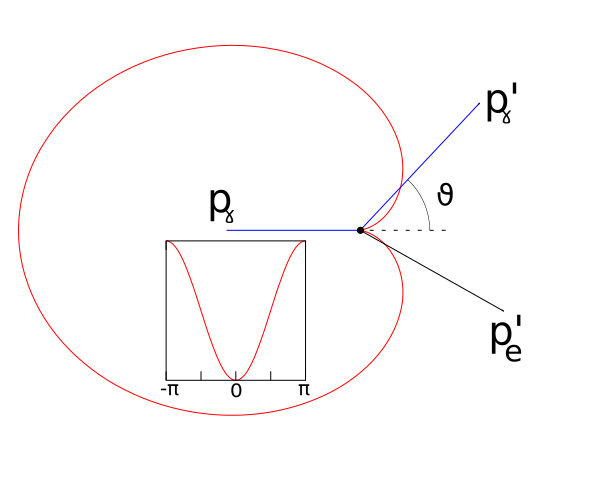
\includegraphics[scale=0.5]{immagini/fisica3/compton}
	\caption{Schema dell'effetto Compton. In blu il fotone, in nero l'elettrone.}
	\label{fig:compton}
\end{figure}
Consideriamo un fotone di frequenza $\nu$ incidente su un elettrone a riposo rispetto al nostro sistema di riferimento. Si osserva che il fotone viene scatterato con un angolo $\theta$ rispetto alla direzione iniziale e con frequenza diversa $\nu'\neq\nu$. Consideriamo un urto relativistico, imponendo la conservazione dell'energia e della quantità di moto, ricordando che:
\begin{equation}
	E^2=(m_0c^2)^2+(pc)^2=E_0^2+(pc)^2
	\label{compton01}
\end{equation}
con $E_0=m_0c^2$ l'energia a riposo dell'elettrone. Conservazione dell'energia:
\begin{equation}
	E_{e}+E_{\gamma}=E=E'=E_e'+E_{\gamma}'
\end{equation}
l'energia del fotone dalla \eqref{compton01}:
\begin{equation}
	E_{\gamma}=p_\gamma c=h\nu\qquad p_\gamma=\frac{h\nu}{c}=\frac{h}{\lambda}
\end{equation}
quindi la conservazione dell'energia si scrive come:
\begin{equation}
	E_{0}+p_\gamma c=\sqrt{E_0^2+(p_e' c)^2}+p_\gamma'c
\end{equation}
isolando la radice:
\[
	E_{0}+c(p_\gamma-p_\gamma')=\sqrt{E_0^2+(p_e'c)^2}
\]
elevando al quadrato:
\[
	E_0^2+c^2(p_\gamma^2+p_\gamma'^2-2p_\gamma p_\gamma')+2E_0c(p_\gamma-p_\gamma')=E_0^2+(p'_ec)^2
\]
\begin{equation}
	c^2(p_\gamma^2+p_\gamma'^2-2p_\gamma p_\gamma')+2E_0c(p_\gamma-p_\gamma')=(p'_ec)^2
	\label{compton03}
\end{equation}
la conservazione della quantità di moto:\
\begin{equation}
	\ve p_\gamma=\ve p=\ve p'=\ve p_\gamma'+\ve p_e'
\end{equation}
passando ai moduli possiamo trovare il momento dell'elettrone:
\begin{equation}
	p_e'^2=p_\gamma^2+p_\gamma'^2-2p_\gamma p_\gamma'\cos\theta
\end{equation}
ricavando dalla \eqref{compton03} $p_e'^2$:
\begin{equation}
	p_e'^2=p_\gamma^2+p_\gamma'^2-2p_\gamma p_\gamma'+2\frac{E_0}{c}(p_\gamma-p_\gamma')
\end{equation}
il sistema di due equazioni ha 4 incognite ($p_e'$, $p_\gamma$, $p_\gamma'$ e $\theta$). Sottraendo le ultime due equazioni:
\begin{equation}
	-2p_\gamma p_\gamma'\cos\theta=-2p_\gamma p_\gamma'+2\frac{E_0}{c}(p_\gamma-p_\gamma')
\end{equation}
semplificando:
\begin{equation}
	p_\gamma p_\gamma'(1-\cos\theta)=\frac{E_0}{c}(p_\gamma-p_\gamma')
\end{equation}
sostituendo $p_\gamma=\frac{h\nu}{c}=\frac{h}{\lambda}$ e analogamente per $p_\gamma'$:
\begin{equation}
	\frac{h}{\lambda}\frac{h}{\lambda'}(1-\cos\theta)=\frac{E_0}{c}\left(\frac{h}{\lambda}-\frac{h}{\lambda'}\right)
\end{equation}
sostituendo $E_0=m_\mathrm{e}c^2$ con $m_\mathrm{e}$ la massa a riposo dell'elettrone:
\begin{equation}
	\frac{h^2}{\lambda\lambda'}(1-\cos\theta)=m_\mathrm{e}ch\left(\frac{\lambda'-\lambda}{\lambda\lambda'}\right)
\end{equation}
si trova:
\begin{equation}
	\lambda'-\lambda=\frac{h}{m_\mathrm{e}c}\left(1-\cos\theta\right)=\lambda_c\left(1-\cos\theta\right)
\end{equation}
che ha $\infty^{4-2}=\infty^2$ soluzioni. La quantità:
\begin{equation}
	\lambda_c=\frac{h}{m_\mathrm{e}c}=2\pi\alpha a_0
\end{equation}
è chiamata lunghezza d'onda di Compton per l'elettrone. La lunghezza d'onda finale è sempre maggiore o uguale a quella iniziale, questo significa che la frequenza e l'energia finale del fotone è sempre minore o uguale a quella iniziale, come ci si aspetta dalla conservazione dell'energia. Come si nota dalla figura \ref{fig:compton} l'effetto è massimo indietro e nullo in avanti.
\index{effetto!Compton|)}
\section{Numeri quantici}
\begin{description}
	\item[$n$]
		è il numero quantico principale, nell'atomo di idrogeno di Bohr è l'unico numero quantico, ed è legato all'energia dell'orbita.
	\item[$l$]
		è il numero quantico angolare, infatti:
		\begin{equation}
			L=\sqrt{l(l+1)}\hslash
		\end{equation}
		con $L$ il modulo del momento angolare totale dell'elettrone. Esso può variare tra:
		\begin{equation}
			0\leq l\leq n-1
		\end{equation}
		ad $l=0$ corrisponde un'oscillazione armonica centrata sul nucleo. Più $l$ è grande e più l'orbita è circolare. In spettroscopia gli stati corrispondenti a diversi $l$ hanno un nome: $l=0$ $S$ (sharp), $l=1$ $P$ (principal), $l=2$ $D$ (diffuse), $l=3$ $F$ (fundamental). Per $l>3$ si segue l'ordine alfabetico.
	\item[$m$]
		è legato a:
		\begin{equation}
			L_z=m\hslash
		\end{equation}
		con $L_z$ la componente $z$ del momento angolare dell'elettrone. Fissato $l$ $m$ può variare:
		\begin{equation}
			-l\leq m\leq l
		\end{equation}
		ci sono quindi $2l+1$ possibili orientazioni per il momento angolare. Il momento angolare non può mai avere direzione $z$, quindi $L_z<L$.
\end{description}
\subsection{Regole di selezione}
Ogniqualvolta un elettrone cambia orbitale deve rispettare le regole di selezione:
\begin{subequations}
	\begin{gather}
		\Delta m=0,\pm 1\\
		\Delta l=\pm 1
	\end{gather}
\end{subequations}
\section{Momento magnetico}
\subsection{Orbitale}
\label{momento_magnetico_orbitale}
Consideriamo un elettrone in un atomo di idrogeno. Con il suo moto circolare produce un campo dipolo magnetico:
\begin{equation}
	\ve\mu=Si\ve n=\pi r^2 \frac{qv}{2\pi r}\ve n=-\frac{1}{2}evr\ve n
\end{equation}
mentre il momento angolare:
\begin{equation}
	\ve L=\ve r\times m\ve v=m_\mathrm{e}vr\ve n
\end{equation}
quindi hanno la stessa direzione e in particolare:
\begin{equation}
	\ve \mu=-\frac{e}{2m_\e}\ve L
\end{equation}
poiché il modulo del momento angolare è quantizzato:
\begin{equation}
	\mu=\frac{e}{2m_\e}L=\frac{e\hslash}{2m_\e}\sqrt{l(l+1)}=\sqrt{l(l+1)}\mu_B
\end{equation}
con $\mu_B$ un magnetone di Bohr\index{magnetone!di Bohr}:
\begin{equation}
	\mu_B=\frac{e\hslash}{2m_\e}
\end{equation}
mentre la componente $z$:
\begin{equation}
	\mu_z=-\frac{q}{2m_\e}L_z=-\frac{e\hslash}{2m_\e}m=-m\mu_B
\end{equation}
\subsection{Esperimento Stern--Gerlach\index{Stern}\index{Gerlach}\index{esperimento!Stern--Gerlach}}
Nell'esperimento Stern--Gerlach si mostra l'esistenza di un altro momento magnetico, quello intrinseco o di spin. Un fascio di molecole collimate vengono fatte passare in una regione in cui il campo magnetico diretto come l'asse $z$ ha un gradiente lungo l'asse $z$. In generale la forza su un dipolo è\footnote{vedi \ref{forza_dipolo100} a pag.\@\pageref{forza_dipolo100}}:
\begin{equation}
	\ve F=\left(\ve \mu\cdot\ve\nabla\right)\ve B
\end{equation}
essendo il gradiente diretto nella direzione $z$ ed esendo $\ve B=B\ver k$:
\begin{equation}
	\ve F=\left(\mu_x\frac{\partial}{\partial x}+\mu_y\frac{\partial}{\partial y}+\mu_z\frac{\partial}{\partial z}\right)B\ver k=\mu_z\frac{\partial B}{\partial z}\ver k
\end{equation}
sull'atomo viene anche esercitato un momento:
\begin{equation}
	\ve\tau=\ve\mu\times\ve B
\end{equation}
che tende ad orientare il momento magnetico nella direzione del campo, cioè la direzione $z$. Poiché l'atomo ha anche un $\ve L\neq 0$ allora $\ve L$ precede intorno alla direzione $z$ sotto l'azione del campo magnetico.
\begin{figure}[htbp]
	\centering
	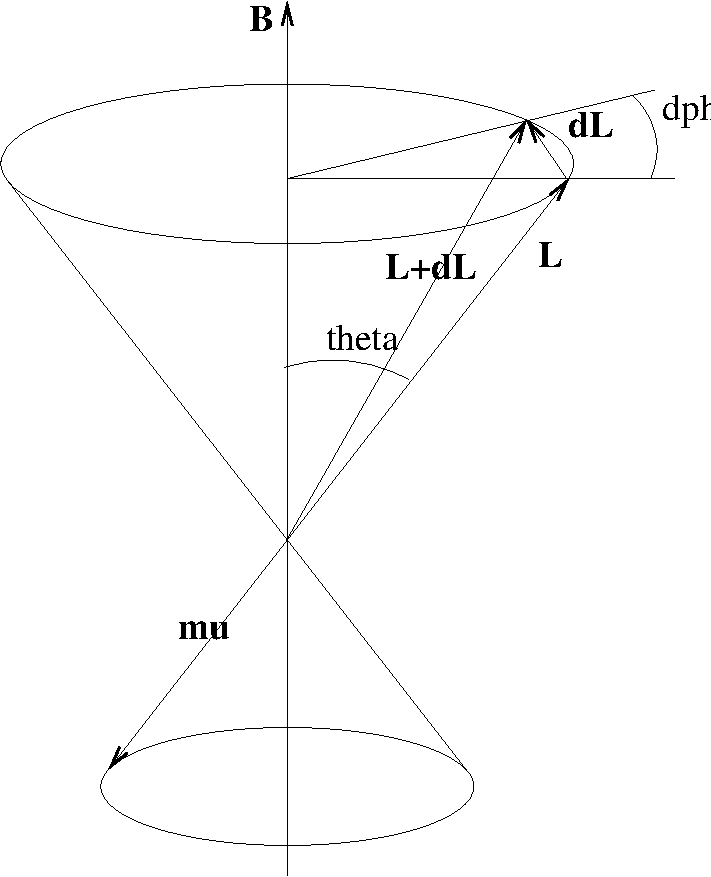
\includegraphics[scale=0.5]{immagini/fisica3/precessione01}
	\label{precessione del momento angolare}
\end{figure}
geometricamente:
\begin{equation}
	\ud L=L\sin\theta\ud\phi
\end{equation}
\begin{equation}
	\frac{\ud\ve L}{\ud t}=\ve\tau=\ve\mu\times\ve B=-\frac{e}{2m_\e}\ve L\times\ve B
\end{equation}
La variazione di $\ve L$ nel tempo è perpendicolare a $\ve L$. Per i moduli:
\begin{equation}
	\frac{\ud L}{\ud t}=-\frac{e}{2m_\e}LB\sin\theta
\end{equation}
Si definisce pulsazione di Larmor la pulsazione della rotazione di $\ve L\neq 0$:
\begin{equation}
	\omega_L=\frac{\ud\phi}{\ud t}=\frac{\ud L}{\ud t}\frac{1}{L\sin\theta}=\frac{eLB\sin\theta\ud t}{2m_\e L\sin\theta}=\frac{eB}{2m_\e}
\end{equation}
Gli atomi infine collidono su uno schermo dove vengono rilevati. L'energia potenziale di un dipolo magnetico nel campo esterno:
\begin{equation}
	W=-\ve\mu\cdot\ve B=-\mu_zB_z=m_l\mu_B B_z=m_l\frac{e\hslash}{2m_\e} B_z=\hslash\omega_L m_l
\end{equation}
che rappresenta anche la variazione di energia $\Delta E$ rispetto ad un elettrone che non è in un campo magnetico.

Classicamente, senza la quantizzazione, ci si aspetterebbe un continuo di possibili traiettorie. Per ogni possibile valore di $\mu_z$ si avrebbe una traiettoria diversa. Considerando la quantizzazione $\mu_z=-m\mu_B$ ci si aspetterebbe delle righe. Potendo $m$ assumere i valori $-l\leq m\leq l$ ci si aspettano $(2l+1)$ righe. Usando idrogeno nello stato fondamentale $n=1, l=0$ ci si aspetta una sola riga, con $l=1$ tre righe corrispondenti ai possibili valori $m=-1,0,1$. Nell'esperimento usando idrogeno nello stato fondamentale si osservarono 2 linee al posto della singola aspettata. Infatti questo stato $\mu_z=-m\mu_B=0$, cioè non c'è momento orbitale. Bisogna ipotizzare che ci sia un altro momento responsabile della presenza di due linee, lo spin $\mu_s=\pm\frac{1}{2}\hslash$.
\subsection{Momento angolare intrinseco}
Per interpretare l'esperimento di Stern--Gerlac si aggiunge un momento angolare intrinseco all'elettrone, usando un nuovo numero quantico, il numero quantico del momento angolare intrinseco:
\begin{equation}
	s=\frac{1}{2}
\end{equation}
che ha (in analogia con $l$ e $m=m_l$):
\begin{equation}
	2s+1=2
\end{equation}
stati possibili. Il momento angolare intrinseco vale in modulo:
\begin{equation}
	S=\sqrt{s(s+1)}\hslash=\frac{\sqrt{3}}{2}\hslash
\end{equation}
come $L=\sqrt{l(l+1)}\hslash$. La componente $z$:
\begin{equation}
	S_z=m_s\hslash
\end{equation}
con $m_s=\pm 1/2$ in analogia con $L_z=m_l\hslash$. Corrispondente al momento angolare intrinseco esiste un momento magnetico intrinseco:
\begin{equation}
	\ve \mu_s=-\frac{e}{2m_\e}g\ve S\simeq -\frac{e}{m_\e}\ve S
\end{equation}
diversamente dal momento orbitale $g\neq 1$, ma è circa 2. La componente $z$ del momento magnetico intrinseco:
\begin{equation}
	\mu_{sz}=-\frac{e}{2m_\e}g S_z=-\frac{e}{2m_\e}gm_s\hslash\simeq-\frac{e}{m_\e}m_s\hslash
\end{equation}

Il momento magnetico totale dell'elettrone in un atomo:
\begin{equation}
	\ve\mu=\ve\mu_L+\ve\mu_s=-\frac{e}{2m_\e}\left(\ve L+g\ve S\right)\simeq-\frac{e}{2m_\e}\left(\ve L+2\ve S\right)
\end{equation}
\subsubsection{interpretazione esperimento Stern--Gerlac}
Nell'esperimento Stern--Gerlac $l=0$, quindi $\ve L=\sqrt{l(l+1)}\hslash=0$ e poiché $m_l=0$ $\mu_L=-m_l\mu_B=0$ allora il momento magnetico totale:
\begin{equation}
	\ve\mu=\ve\mu_s=-\frac{e}{2m_\e}g\ve S\simeq-\frac{e}{m_\e}\ve S
\end{equation}
è dato solo dal momento magnetico di spin. Il modulo sarà:
\begin{equation}
	\mu=\frac{e}{m_\e}S=\frac{\sqrt{3}e}{2 m_\e}\hslash
\end{equation}
mentre la componente $z$:
\begin{equation}
	\mu_z=\mu_{sz}=-\frac{e}{m_\e}m_s\hslash=\pm\frac{e\hslash}{2m_\e}=\pm\mu_B
\end{equation}
Essendoci due possibili stati si osserveranno due righe distinte.
\section{Momento angolare totale}
Il momento angolare totale $\ve J$ è la somma dei momenti angolari orbitale e intrinseco:
\begin{equation}
	\ve J=\ve L+\ve S
\end{equation}
$\ve J$ si conserva durante le interazioni. Il suo modulo è quantizzato mediante:
\begin{equation}
	J=\sqrt{j(j+1)}\hslash
\end{equation}
con:
\begin{equation}
	j=|l-s|,|l-s|+1,\ldots,|l+s|
	\label{varl14}
\end{equation}
mentre la componente $z$:
\begin{equation}
	J_z=m_j\hslash
\end{equation}
con
\begin{equation}
	m_j=-j,-j+1,\ldots,j
\end{equation}
Nella notazione spettroscopica spesso il numero quantico $j$ viene riportato in pedice alla lettera rappresentante l'orbitale.
\begin{Es}[$2p$]
	Lo stato $2p$ cioè $n=2$, $l=1$ dell'idrogeno ha $j$ che può assumere i valori secondo l'equazione \eqref{varl14}:  $j=|l-s|=|1-\frac{1}{2}|=\frac{1}{2}$ o $j=|l+s|=|1+\frac{1}{2}|=\frac{3}{2}$. Quindi la notazione spettroscopica sarà: $2p_{1/2}$ (per $j=\frac{1}{2}$) o $2p_{3/2}$ (per $j=\frac{3}{2}$).
\end{Es}
\begin{Es}[stato fondamentale dell'idrogeno]
	Calcoliamo quanto vale $J$ e $J_z$ per lo stato fondamentale dell'idrogeno. In questo stato $l=0$. $j$ può valere solo
	\[
		j=|l-s|=|l+s|=\frac{1}{2}
	\]
	mentre $m_j$ può valere $\pm\frac{1}{2}$.
	Quindi:
	\[
		J=\sqrt{j(j+1)}\hslash=\frac{\sqrt{3}}{2}\hslash\qquad J_z=m_s\hslash=\pm\frac{\hslash}{2}
	\]
\end{Es}
\begin{Es}[stato $p$]
	Calcoliamo quanto vale $J$ per lo stato $p$ dell'idrogeno $l=1$. Quindi $j$ può assumere i valori:
	\[
		j=|1-\frac{1}{2}|,\ldots,|1+\frac{1}{2}|=\frac{1}{2},\frac{3}{2}
	\]
	e allora:
	\[
		J=\sqrt{j(j+1)}\hslash=\frac{\sqrt{3}}{2}\hslash,\frac{\sqrt{15}}{2}\hslash
	\]
	se $j=\frac{1}{2}$ allora $m_j=\pm\frac{1}{2}$ e $J_z=\pm\frac{1}{2}\hslash$; se $j=\frac{3}{2}$ allora $m_j=\pm\frac{3}{2},\pm\frac{1}{2}$ e $J_z=\pm\frac{3}{2}\hslash$ o $J_z=\pm\frac{1}{2}\hslash$.
\end{Es}
\subsection{Somma di momenti}
Sia $\ve J_1$ un momento (orbitale, intrinseco o una combinazione) e $\ve J_2$ un altro. Il vettore risultante sarà $\ve J=\ve J_1+\ve J_2$. Il suo modulo sarà:
\begin{equation}
	J=\sqrt{j(j+1)}\hslash
\end{equation}
con $j$ che può assumere i valori:
\begin{equation}
	j=|j_1-j_2|,|j_1-j_2|+1,\ldots,|j_1+j_2|
	\label{jequation}
\end{equation}
\begin{Es}[somma di spin]
	Sommiamo il momento intrinseco di due elettroni $S_1$ e $S_2$. Essendo $S_1=\sqrt{s(s+1)}\hslash$ usando la notazione dell'equazione \eqref{jequation} $j_1=\frac{1}{2}$ e analogamente $j_2=\frac{1}{2}$. Allora:
	\[
		\ve S=\ve S_1+\ve S_2\qquad S=\sqrt{j(j+1)}\hslash
	\]
	con $j=0,1$, che corrisponde allo spin antiparallelo e parallelo.
\end{Es}
\section{Interazione spin--orbita\index{interazione!spin--orbita}}
Stati atomici con gli stessi numeri quantici $n$ e $l$, ma diversi $j$ hanno una lieve differenza di energia a causa dell'interazione dello spin dell'elettrone con il momento orbitale. Il risultato è una leggera separazione delle linee spettrali, chiamata separazione di struttura fine.

Se $l\neq 0$ allora il moto dell'elettrone crea un campo magnetico interno $\ve B_\text{int}$ (se $\ve l=0$ allora $L=0$). Consideriamo il sistema di riferimento dell'elettrone in cui vediamo il nucleo con un momento angolare $\ve L$. Il campo magnetico interno è orientato nella stessa direzione del momento angolare orbitale. Il momento magnetico intrinseco $\ve\mu_s$ dovuto al momento angolare intrinseco $\ve S$ interagisce con il campo interno $\ve B_\text{int}$, causando una differenza di energia dello stato $\Delta E$:
\begin{equation}
	\Delta E=-\ve\mu_s\cdot\ve B_\text{int}=\frac{e}{2m_\e}g\ve S\cdot\ve B_\text{int}=C\ve S\cdot\ve L
\end{equation}
con $C$ una costante positiva. $\Delta E$ dipende dall'orientazione di $\ve S$ rispetto a $\ve L$. Se $\ve S$ è parallelo con $\ve L$ allora l'incremento è positivo, quando invece $\ve S$ è antiparallelo con $\ve L$ è negativo.

Considerando l'orbitale $2p$ questo viene diviso in due livelli energetici: $2P_{\frac{3}{2}}$ con energia maggiore e $2P_{\frac{1}{2}}$ con energia minore. Quindi la riga singola in realtà appare come una doppia linea.
\subsection{Approssimazione quantitativa}
Consideriamo l'orbita 2p. Il campo magnetico generato una una spira al centro è:
\begin{equation}
	B=\frac{\mu_0}{2}\frac{I}{r}=\frac{\mu_0}{2}\frac{ev}{4\pi r^2}
\end{equation}
lungo l'asse $z$. Il momento angolare intrinseco lungo l'asse $z$:
\begin{equation}
	S_z=m_s\hslash=\pm\frac{1}{2}\hslash
\end{equation}
L'energia di interazione:
\begin{equation}
	\Delta W=-\ve\mu_S\cdot\ve B=\frac{e}{2m_\e}g\ve S\cdot\ve B\simeq\pm\frac{e}{2m_\e}2\frac{\hslash}{2}\frac{\mu_0ev}{8\pi r^2}
\end{equation}
ricordando che $\alpha=\frac{e^2}{\giorgi\hslash c}$ e usando $c=\frac{1}{\sqrt{\varepsilon_0\mu_0}}$:
\begin{equation}
	\Delta W=\frac{e^2\hslash\mu_0v}{16m_\e\pi r^2}=\pm\frac{e^2\hslash v}{16m_\e c^2\pi\varepsilon_0 r^2}=\frac{\hslash^2v\alpha}{4m_\e r^2 c}
\end{equation}
dalla \eqref{betabohr} $\frac{v}{c}=\frac{Z}{n}\alpha$ e $Z=1$, $n=2$:
\begin{equation}
	\frac{v}{c}=\frac{\alpha}{2}
\end{equation}
sostituendo:
\begin{equation}
	\Delta W=\frac{\hslash^2}{4m_\e r^2}\frac{\alpha^2}{2}
\end{equation}
il raggio:
\begin{equation}
	r=n^2a_0=4\frac{\hslash }{\alpha m_\e c}
\end{equation}
sostituendo:
\begin{equation}
	\Delta W=\frac{\hslash^2\alpha^2 m_\e^2 c^2}{4m_\e 16\hslash^2}\frac{\alpha^2}{2}=\frac{\alpha^4m_\e c^2}{128}
\end{equation}
questo è la differenza di energia tra i livelli $P_\frac{1}{2}$ e $P_\frac{3}{2}$ dell'idrogeno rispetto al $2P$ senza considerare l'interazione spin orbita. La differenza di energia tra i due stati sarà quindi il doppio:
\begin{equation}
	\Delta W'\simeq\frac{\alpha^4m_\e c^2}{64}
\end{equation}
